\documentclass[12pt,spanish]{article}
\usepackage[spanish]{babel}
\usepackage{graphicx}
\usepackage{color}
\usepackage{xcolor}
\usepackage{colortbl}
\usepackage{amsthm,thmtools}
\usepackage{dirtytalk}
\usepackage{multirow}
\usepackage{amsmath}
\usepackage{subcaption}
\usepackage{adjustbox}
\usepackage{amsmath}
\usepackage{centernot}
\usepackage{mathtools}
\usepackage{multirow}
\usepackage[hidelinks]{hyperref}
\usepackage{caption}
\usepackage{eurosym} % para el euro
\usepackage{amsthm}
\usepackage{multicol}
\usepackage{float}
\usepackage{amsfonts}
\usepackage{titling}
\usepackage{soul}
\usepackage{listings}
\usepackage{array}
\usepackage{tikz}
\usetikzlibrary{shapes.geometric, arrows, chains, calc,positioning,fit,decorations.pathreplacing}
\usepackage[framemethod=tikz]{mdframed}

\graphicspath{ {../img/}}
\selectlanguage{spanish}
\usepackage[utf8]{inputenc}
\usepackage{graphicx}
\usepackage[a4paper,left=3cm,right=2cm,top=2.5cm,bottom=2.5cm]{geometry}

\newenvironment{solution}{
	\par
	\textbf{Solución}
	\par
	\begin{center}
}
{
	\end{center}
}

\lstset{
  breaklines=true,
  postbreak=\mbox{\textcolor{red}{$\hookrightarrow$}\space},
}


\title{Ingeniería de Servidores}
\setlength{\droptitle}{10em}
\author{Carlos Sánchez Páez}

\makeindex
\begin{document}
\definecolor{light-gray}{gray}{0.95}
\lstset{columns=fullflexible,basicstyle=\ttfamily}
\surroundwithmdframed[
  hidealllines=true,
  backgroundcolor=light-gray,
  innerleftmargin=0pt,
  innertopmargin=0pt,
  innerbottommargin=0pt]{lstlisting}


\begin{titlepage}

 \newlength{\centeroffset}
 \setlength{\centeroffset}{-0.5\oddsidemargin}
 \addtolength{\centeroffset}{0.5\evensidemargin}
 \thispagestyle{empty}

 \noindent\hspace*{\centeroffset}
 \begin{minipage}{\textwidth}

  \centering
  
\includegraphics[width=0.9\textwidth]{logo_ugr.jpg}\\[1.4cm]

  \textsc{ \Large Ingeniería de Servidores\\[0.2cm]}
  \textsc{GRADO EN INGENIERÍA INFORMÁTICA}\\[1cm]

  {\Huge\bfseries Resumen del temario\\}
 \end{minipage}

 \vspace{1.5cm}
 \noindent\hspace*{\centeroffset}
 \begin{minipage}{\textwidth}
  \centering

  \textbf{Autor}\\ {Carlos Sánchez Páez}\\[2.5ex]
  
\includegraphics[width=0.4\textwidth]{etsiit_logo.png}\\[0.1cm]
  \vspace{1.5cm}
  
\includegraphics[width=0.15\textwidth]{atc.jpg}\\[0.1cm]
  \vspace{1cm}
  \textsc{Escuela Técnica Superior de Ingenierías Informática y de Telecomunicación}\\
  \vspace{1cm}
  \textsc{Curso 2019-2020}
 \end{minipage}
\end{titlepage}
\thispagestyle{empty}
\newpage
\tableofcontents{}
\newpage
\listoffigures
\thispagestyle{empty}
\newpage

\section{Tema 1. Introducción a la Ingeniería de Servidores}

\subsection{¿Qué es un servidor?}

Un \textbf{sistema informático} es un conjunto de elementos \textit{hardware} (componentes físicos), \textit{software} (componentes lógicos) y \textit{peopleware} (recursos humanos) que permite obtener, procesar y almacenar información.\\
Los sistemas informáticos se pueden clasificar atendiendo a varios factores:
\begin{itemize}
	\item Según el nivel de paralelismo (\textit{SISD},\textit{SIMD},\textit{MISD} o \textit{MIMD})
	\item Según su uso (propósito general o específico)
	\item[*] Si son servidores, según la arquitectura de servicio (sistema aislado, cliente-servidor, \emph{n} capas o cliente-cola-cliente)
\end{itemize}

\subsubsection{Según su nivel de paralelismo}

\begin{itemize}
	\item \textit{SISD}: \textbf{S}ingle \textbf{I}nstruction \textbf{S}ingle \textbf{D}ata
	\item \textit{SIMD}: \textbf{S}ingle \textbf{I}nstruction \textbf{M}ultiple \textbf{D}ata
	\item \textit{MISD}: \textbf{M}ultiple \textbf{I}nstruction  \textbf{S}ingle \textbf{D}ata
	\item \textit{MIMD}: \textbf{M}ultiple \textbf{I}nstruction  \textbf{M}ultiple \textbf{D}ata
\end{itemize}
\begin{figure}[H]
	\centering
	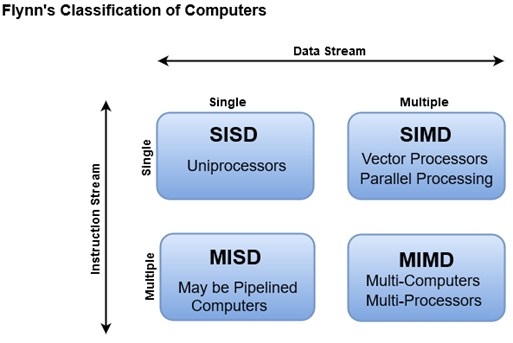
\includegraphics[width=0.5\textwidth]{comparacion_paralelismo.png}
	\caption{Sistemas informáticos según su nivel de paralelismo}
\end{figure}

\subsubsection{Según su uso}

\begin{itemize}
	\item De \textbf{uso general}: sirven para ejecutar diversas aplicaciones (PC sobremesa, portátil).
	\item De \textbf{uso específico}: ejecutan una función concreta.
	\begin{itemize}
		\item \textbf{Sistemas empotrados (\textit{embedded systems})}. Son sistemas acoplados a otro dispositivo o aparato que realizan una o varias funciones dedicadas. Suelen tener grandes restricciones de tamaño, tiempo de respuesta, etc. Suelen estar formados por un microprocesador, memoria y una amplia gama de interfaces de comunicación.Ejemplo: taxímetro, cámara de vigilancia, lavadora, etc.
		\item \textbf{Servidores}. Son sistemas informáticos que forman parte de una red y proporcionan servicios a otros sistemas informáticos (clientes). Puede ser cualquier computador o \textit{clúster} (agrupación de computadores que son percibidos externamente como uno solo).
	\end{itemize}
\end{itemize}

Hay varios tipos de servidores:
\begin{itemize}
	\item \textbf{Servidor de archivos}: permite el acceso remoto a archivos almacenados o directamente accesibles por él.
	\item \textbf{Servidor web}: almacena documentos HTML, imágines, etc. y distribuye el contenido a los clientes que lo soliciten.
	\item \textbf{Servidor de base de datos}: provee servicios de base de datos a otros programas o sistemas.
	\item \textbf{Servidor de \textit{e-commerce}}: cumple o procesa transacciones comerciales. Valida al cliente y genera un pedido al servidor de bases de datos.
	\item \textbf{Servidor de impresión}: controla una o más impresoras y acepta trabajos de impresión de los clientes de la red.
	\item \textbf{Servidor de correo electrónico}: almacena, envía, recibe, etc. correos electrónicos para los clientes de la red.
\end{itemize}

\subsubsection{Según su arquitectura de servicio}
\begin{itemize}
	\item \textbf{Sistema aislado}: es un sistema que no interactúa con otros. La arquitectura es monolítica y no se distribuye la información
	\item \textbf{Arquitectura cliente-servidor}: las tareas se reparten entre los servidores (reciben solicitudes) y los clientes (remiten solicitudes). Los nodos son los servidores y los clientes.
	\item \textbf{Arquitectura cliente-servidor de \emph{n} capas}: es una arquitectura cliente-servidor que tiene \emph{n} tipos de nodos en la red, por lo que se mejora la distribución de la carga (mejorando la escalabilidad). Sus principales puntos negativos son la sobrecarga de la red que conlleva y la dificultad de programación y administración.\\
	Ejemplo de arquitectura de 3 capas:
	\begin{enumerate}
		\item Servidores que interactúan con los clientes.
		\item Servidores de \textit{e-commerce} que procesan los datos para los servidores de la capa 1.
		\item Servidores de bases de datos que buscan, gestionan y almacenan los datos para los servidores de la capa 2.
	\end{enumerate}
	\item \textbf{Arquitectura cliente-cola-cliente}: el servidor únicamente pone en contacto a los clientes y sincroniza el sistema, mientras que los clientes se encargan de cooperar para realizar la función necesaria. La arquitectura \textit{P2P} está basada en este concepto. Ejemplos: \textit{Skype}, \textit{eMule}, \textit{BitTorrent}.
\end{itemize}

\subsection{Fundamentos de la Ingeniería de Servidores}

Un servidor se compone de:
\begin{itemize}
	\item Recursos físicos (placa base, memoria, CPU, etc.).
	\item Recursos lógicos (sistema operativo, aplicaciones).
	\item Recursos humanos (administración).
	\item Requisitos funcionales (prestaciones, seguridad, mantenimiento, disponibilidad, extensibilidad, escalabilidad, coste, fiabilidad...)
\end{itemize}

Las \textbf{prestaciones} cuantifican la velocidad con la que se realiza una determinada cantidad de trabajo o carga (\textit{workload}). Aquel servidor que realiza la misma carga de trabajo en menor tiempo es el que mayores prestaciones tiene.\\
Las medidas fundamentales para medir las prestaciones de un servidor son:
\begin{itemize}
	\item \textbf{Tiempo de respuesta} o \textbf{latencia}. Tiempo desde que se solicita una tarea al servidor hasta que finaliza. Por ejemplo: tiempo de ejecución de un programa, de acceso al disco, etc.
	\item \textbf{Productividad} (\textit{throughput}) o \textbf{ancho de banda} (\textit{bandwidth}). Cantidad de trabajo realizado por el servidor por unidad de tiempo. Por ejemplo: programas ejecutados por hora o páginas por hora servidas en el caso de un servidor web.
\end{itemize}

Los principales elementos que afectan a las prestaciones de un servidor son los siguientes:
\begin{itemize}
	\item Hardware del sistema (características y configuración).
	\item Parámetros del sistema operativo (configuración de memoria virtual, políticas de planificación...) y diseño de los programas (acceso a E/S, fallos de caché...).
	\item Actualización de componentes (reemplazar por dispositivos más rápidos) y configuración de dispositivos.
	\item Ajuste o sintonización del SO y los programas.
	\item Distribución de carga (\textit{load balancing}): dar mayor carga a los dispositivos más rápidos.
\end{itemize}

\subsubsection{Requisitos funcionales de un servidor}

\begin{itemize}
	\item \textbf{Disponibilidad} (\textit{Availability}). Un servidor está disponible si está en estado operativo.\\ El tiempo de inactividad (\textit{downtime}) es la cantidad de tiempo en la que el sistema no está disponible. Puede ser de dos tipos:
	\begin{itemize}
		\item Planificado (actualizaciones de hardware o software que no se puedan realizar en caliente).
		\item No planificado (a causa de algún fallo).

		$\rightarrow$ Si el sistema tiene \emph{alta disponibilidad} será \emph{tolerante a fallos}.
	\end{itemize}
	\newpage
	Algunas soluciones para aumentar la disponibilidad son:
	\begin{itemize}
		\item Reemplazo en caliente de los componentes (\textit{hot-swapping}).
		\item Sistemas redundantes de discos (\textit{RAID}), alimentación y red.
		\item Sistemas distribuidos.
	\end{itemize}
	\item \textbf{Fiabilidad} (\textit{Reliability}). Un sistema es fiable cuando realiza su actividad sin errores. Se aplica más a componentes por separado. El \textbf{MTTF} (\textit{\textbf{M}ean \textbf{T}ime \textbf{T}o \textbf{F}ailure}) es el tiempo medio que tiene un sistema hasta que ocurre un error. Los mecanismos para asegurar la fiablilidad son la comprobación (\textit{checksums}, bits de paridad, etc.)
	\item \textbf{Seguridad}. Un servidor debe ser seguro ante:
	\begin{itemize}
		\item La incursión de individuos no autorizados (\textit{confidencialidad}).
		\item La corrupción o alteración no autorizada de datos (\textit{integridad}).
		\item Las interferencias (ataques) que impidan el acceso a los recursos.
	\end{itemize}
	Las principales soluciones son la encriptación de datos, el uso de cortafuegos y la autenticación segura de usuarios.
	\item \textbf{Extensibilidad-expansibilidad}. Es la facilidad que ofrece el sistema para aumentar sus características o recursos (tener bahías libres para discos duros o memoria, uso de sistemas operativos modulares, uso de interfaces de entrada y salida estándar, etc.). Cualquier solución que facilite la escalabilidad facilita también la extensibilidad.
	\item \textbf{Escalabilidad}. Un servidor es escalable si sus prestaciones pueden aumentar significativamente ante un incremento significativo de la carga. Las soluciones más usadas son la virtualización, la programación paralela y la tecnología \textit{cloud}. Todos los sistemas escalables son extensibles (pero no al revés).
	\item \textbf{Mantenimiento}. Son las acciones que sirven para prolongar el funcionamiento correcto del sistema. Es importante que el servidor sea fácil de mantener (sistema operativo actualizado, garantía de componentes, copias de seguridad, etc.).
	\item \textbf{Coste}. Debemos escoger un diseño que sea asequible y se ajuste al presupuesto teniendo en cuenta el coste hardware, software, de actualizaciones, de personal, de proveedores de red, de alquiler de local y de \textbf{eficiencia energética}. La eficiencia energética es clave ya que reduce en gran cantidad los costes (consumo de potencia, refrigeración) y además ayuda a preservar el medio ambiente. Las soluciones más comunes son:
	\begin{itemize}
		\item Ajuste automático de potencia de los componentes según la carga.
		\item \textit{Free cooling}, aprovechamiento de las bajas temperaturas exteriores para tener refrigeración gratuita.
		\item Fusionar varios servidores con poco uso en un único servidor.
	\end{itemize}

\end{itemize}

\subsection{Comparación conjunta entre prestaciones y coste}

El computador de mejores prestaciones (el más rápido) para un determinado conjunto de programas será el que lo ejecute en menor tiempo.\\

\subsubsection{Tiempos de ejecución mayores o menores}

Sea $t_A$ el tiempo de ejecución de un programa en la máquina A (ídem para $t_B$).
\begin{itemize}
	\item $t_A$ es $\frac{t_A}{t_B}$ veces $t_B$. Por ejemplo, si $t_A=10s$ y $t_B=5s$, $t_A$ es $\frac{10}{5}=2$ veces $t_B$ (el doble).
	\item Igualmente, $t_B$ es $\frac{5}{10}=0.5$ veces $t_A$ (la mitad).
\end{itemize}

El \textbf{cambio relativo de $t_A$ con respecto a $t_B$}; $\Delta t_{A,B}(\%)$ viene dado por:
\[
t_A=t_B + \frac{\Delta t_{A,B}(\%)}{100} * t_B
\]
Es decir, es el porcentaje que le falta a $t_B$ para ser $t_A$.\\
En el ejemplo anterior el cambio relativo de $t_A$ con respecto a $t_B$ es del 100\%. Es decir, a $t_B$ le falta un 100\% de sí mismo (el doble) para llegar a ser $t_A$.\\
De igual forma, el cambio relativo de $t_B$ con respecto a $t_A$ es del -50\% (a $t_A$ le sobra la mitad para ser $t_B$).\\
Usando el lenguaje común podríamos traducir los resultados en:
\begin{itemize}
	\item $t_A$ es un 100\% mayor que $t_B$ y $t_B$ es un 50\% menor que $t_A$.
	\item $t_A$ es 2 veces mayor que $t_B$ (¡ojo! ¡¡''1 vez mayor'' significa igual!!).
\end{itemize}

La velocidad de ejecución de una máquina será inversamente proporcional al tiempo que tarda en ejecutarse. Teniendo ésto en cuenta podemos definir la aceleración (\textit{speedup}) de A con respecto a B de la siguiente forma:
\[
S_B(A)=\frac{v_A}{v_B}=\frac{t_B}{t_A}
\]
El cambio relativo de $v_A$ con respecto de $v_B$ (es decir, el porcentaje de cambio en velocidad al reemplazar A por B) viene dado por:
\[
\Delta v_{A,B}(\%)=(S_B(A) -1) * 100
\]

Supongamos que para un programa, $t_A=36s$ y $t_B=45s$.\\
La ganancia de velocidad de A con respecto a B sería:
\[
S_B(A)=\frac{v_A}{v_B}=\frac{t_B}{t_A}=\frac{45 s}{36 s}=1.25
\]
El cambio relativo de $v_A$ con respecto a $v_B$ (es decir, el porcentaje de mejora) viene dado por:
\[
\Delta v_{A,B}(\%)=(S_B(A)-1) * 100 = (1.25 - 1) * 100 = 0.25 * 100 = 25\%
\]
Usando el lenguaje común diríamos que:
\begin{itemize}
	\item A es 1.25 veces más rápida que B.
	\item A es un 25\% más rápida que B
\end{itemize}
De igual forma:
\[
S_A(B)=\frac{t_A}{t_B}=\frac{36 s}{45 s}=0.8
\]
\[
\Delta v_{B,A}(\%)=(S_A(B)-1) * 100 = (0.8 - 1) * 100 = -0.2 * 100 = -20\%
\]
Es decir, B es un 20\% más lenta que A.

\begin{center}
	¡¡Ojo!! \\
	A es un $x\%$ más rápida que B $\centernot\implies$ B es un $x\%$ más lenta que A.\\
	Por ejemplo, 10 es un 100\% mayor que 5 $\centernot\implies$ 5 es un 100\% menor que 10
\end{center}

Supongamos que en el ejemplo anterior el computador A cuesta 625 \textup{\euro} y el computador B, 550 \textup{\euro}.
\begin{itemize}
	\item A es $\frac{625}{550}=1.14$ veces más caro que B (un 14\% más caro).
	\item ¿Cuál ofrece mejor relación prestaciones/precio para nuestro programa?
	\[
		\frac{Prestaciones_A}{Coste_A}=\frac{v_A}{Coste_A} \propto \frac{\frac{1}{t_A}}{Coste_A}=\frac{\frac{1}{36 s}}{625 \textup{\euro}} = 4.4 * 10^{-5} \frac{s^{-1}}{\textup{\euro}}
	\]

	\[
		\frac{Prestaciones_B}{Coste_B}=\frac{v_B}{Coste_B} \propto \frac{\frac{1}{t_B}}{Coste_B}=\frac{\frac{1}{45 s}}{550 \textup{\euro}} = 4.0 * 10^{-5} \frac{s^{-1}}{\textup{\euro}}
	\]
	Pasamos ahora a comparar ambas relaciones:
	\[
	\frac{\frac{Prestaciones_A}{Coste_A}}{\frac{Prestaciones_B}{Coste_B}} = \frac{4.4 * 10^{-5}}{4.0 * 10^{-5}} = 1.1
	\]
	\item Por tanto, el computador A presenta una mayor relación prestaciones/coste que B (un 1.1 mayor $=$ un 10\% mayor) para nuestro programa.
\end{itemize}


\subsection{Límites en la mejora del tiempo de respuesta}

La mejora dekl tiempo de respuesta no es ilimitada, por lo que debemos saber hacia dónde dirigir los esfuerzos. Por ejemplo, si un programa utiliza la CPU en un 80\% del tiempo y la impresora en un 20\% debemos centrarnos en mejorar la CPU. El planteamiento sería el siguiente:
\begin{itemize}
	\item Un sistema tarda un tiempo $T_{original}$ en ejecutar un programa monohebra.
	\item Mejoramos el sistema reemplazando un componente por otro $k$ veces más rápido.
	\item Este comonente se utilizaba durante una fracción $f$ de $T_{original}$ (si $f=1$, el componente se utilizaba el 100\% del tiempo).
	\item ¿Qué ganancia en prestaciones (\textit{speedup}) hemos conseguido con el cambio?
\end{itemize}
\newpage
\begin{figure}[H]
	\centering
	\begin{tikzpicture}[arrow/.style = {thick,-stealth}]
		\tikzset{set/.style={draw,rectangle,inner sep=0pt,align=center}}
		\node[fit={(0,0) (5,1.5)}, inner sep=0pt, draw=black, thick, fill=blue!20, text centered] (nousado1) { Recurso no utilizado \\($1-f * t_O$)};
		\node[fit={(5,0) (15,1.5)}, inner sep=0pt, draw=black, thick, fill=green!20, text centered] (usado1) {Recurso utilizado ($f * t_O$)};

		\node[fit={(0,-5) (5,-3.5)}, inner sep=0pt, draw=black, thick, fill=blue!20, text centered] (nousado2) { Recurso no utilizado \\($1-f * t_O$)};
		\node[fit={(5,-5) (10,-3.5)}, inner sep=0pt, draw=black, thick, fill=yellow!20, text centered] (usado2) {Recurso utilizado ($\frac{f * t_O}{k}$)};

		\draw [arrow] (5,0) -- (5,-3.5);
		\draw [arrow] (15,0) -- node [below right] {$k$ veces más pequeño} (10,-3.5);

		\draw [decorate,decoration={brace,amplitude=10pt, raise=2.5pt}]	(0,1.5) -- (15,1.5) node [black, midway, sloped, above=0.5cm] {Tiempo original $t_O$};

		\draw [decorate,decoration={brace,amplitude=10pt, raise=2.5pt, mirror}]	(0,-5) -- (10,-5) node [black, midway, sloped, below=0.5cm] {Tiempo mejorado $t_M$};

	\end{tikzpicture}
	\caption{Tiempos original y mejorado}
\end{figure}

\subsubsection{Ley de Amdahl}
¿Cuál es la ganancia en velocidad ($S$) del sistema después de mejorar $k$ veces un componente?
\begin{figure}[H]
	\begin{equation*}
		S=\frac{1}{1-f+\frac{f}{k}}
	\end{equation*}
	\caption{Ley de Amdahl}
\end{figure}
Donde:
\begin{itemize}
	\item Si $f=0 \implies S=1$, por lo que no hay mejora en el sistema (el recurso no se usaba).
	\item Si $f=1 \implies S=k$, el sistema mejora tantas veces como el componente (se usa siempre).
	\item Si $f\to \infty \implies S \to \lim_{k \to \infty} S=\frac{1}{1-f}$
\end{itemize}

Veamos un ejemplo:\\
La utilziación de un disco duro es del 60\% para un programa monohebra. ¿Cuál será la velocidad de ejecución si duplicamos la velocidad del disco?
\[
S=\frac{1}{1-f+\frac{f}{k}} \implies S=\frac{1}{1-0.6+\frac{0.6}{2}}=1.43
\]
Por tanto, el sistema es $1.43$ veces más rápido (un 43\% más rápido que antes).\\
Si sólo nos centráramos en mejorar el disco, la ganancia máxima que podríamos obtener sería:
\[
S_{max}=\lim_{k \to \infty}S=\frac{1}{1-f}=\frac{1}{1-0.6}=2.5
\]
Es decir, el sistema podría llegar a ser $2.5$ veces más rápido (un 150\% más rápido) que antes si sólo mejoramos el disco.

\subsubsection{Generalización de la ley de Amdahl}

Para $n$ mejoras, el \textit{speedup} vendría dado por:

\[
S=\frac{1}{(1-\sum_{i=1}^{n}f_i) + \sum_{i=1}^{n}\frac{f_i}{k_i}}
\]

También podemos calcular la aceleración con una sola mejora en cascada, teniendo en cuenta que debemos recalcular $f$ en cada paso. Sin embargo, es mucho más sencillo aplicar el procedimiento del \hyperref[1.13]{\textbf{ejercicio 1.3}}.
\newpage
\section{Tema 2. Componentes hardware de un servidor}

\subsection{Placa base (\textit{Motherboard})}
Es la tarjeta de circuito impreso (\textit{PCB}) que interconecta los distintos componentes.
\begin{figure}[H]
	\centering
	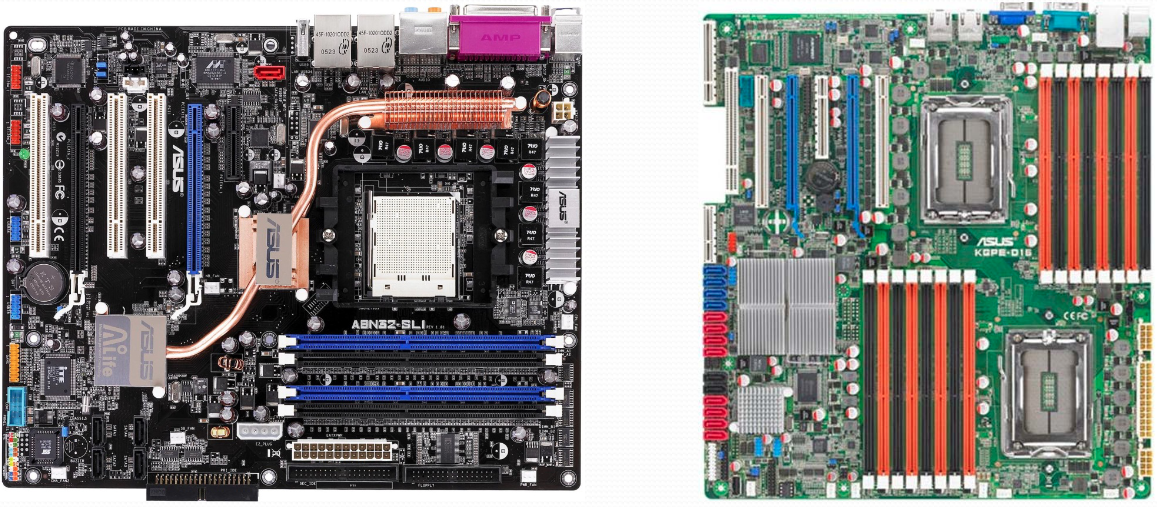
\includegraphics[width=0.5\textwidth]{mobos.png}
	\caption{Dos placas base}
\end{figure}
\subsubsection{Tarjeta de cirtuito impreso}

Está hecha de pistas de cobre rodeadas de un elemento aislante (fibra de vidrio con resina no inflamable).\\
Actualmente, las placas base son multi-capa. A través de unos agujeros (vías) se realiza la conexión de una capa con otra.\\
Las placas base tienen un tamaño (\textit{form factor}) estandarizado: \textit{Standard-ATX}, \textit{Micro-ATX}, \textit{Mini-ITX}...
\begin{figure}[H]
	\centering
	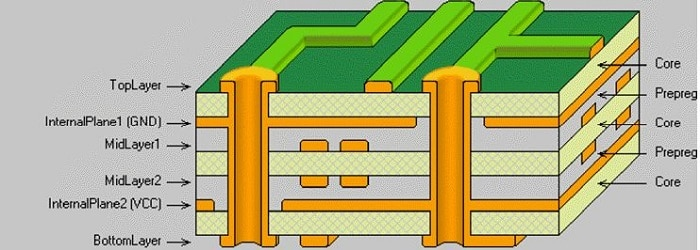
\includegraphics[width=0.5\textwidth]{pcb.jpg}
	\caption{\textit{PCB} multicapa}
\end{figure}

\begin{figure}[H]
	\centering
	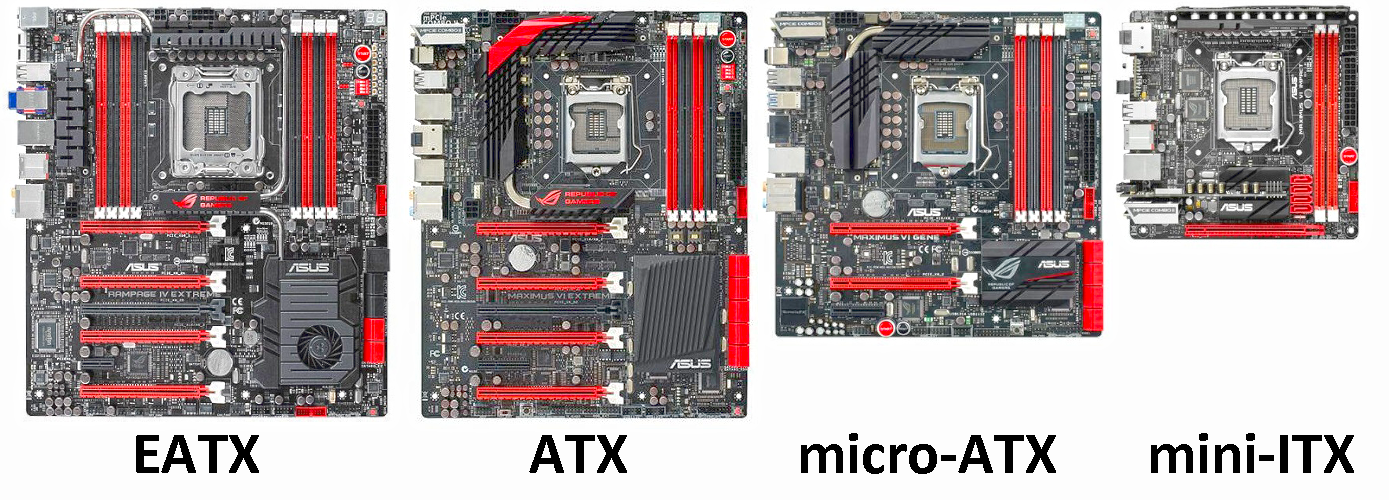
\includegraphics[width=0.5\textwidth]{moboformfactor.png}
	\caption{Distintos factores de forma de placas base}
\end{figure}

\subsubsection{Componentes de una placa base}
\begin{figure}[H]
	\centering
	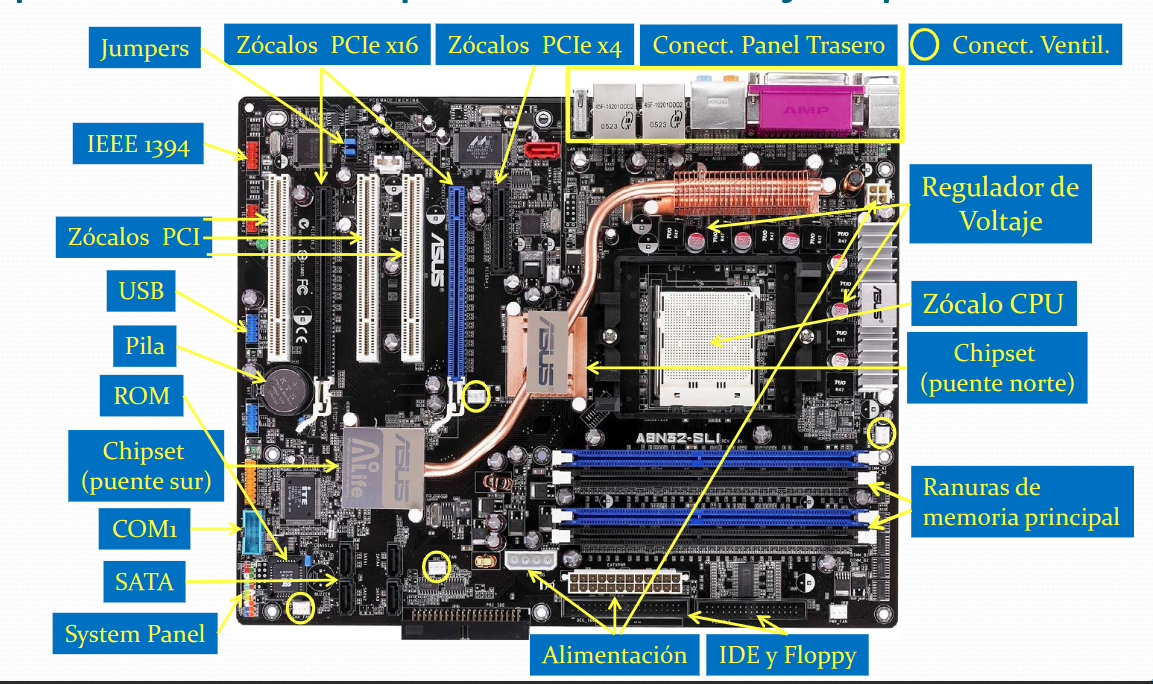
\includegraphics[width=\textwidth]{mobocomponents.png}
	\caption{Componentes de una placa base}
\end{figure}
En el manual de la placa podremos ver un esquema simple de la localización de sus principales componentes:

\begin{figure}[H]
	\centering
	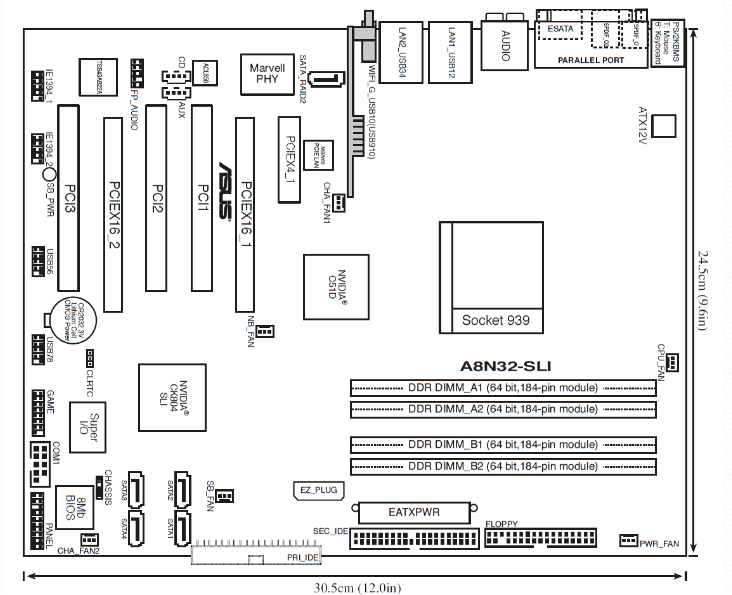
\includegraphics[width=0.75\textwidth]{mobocomponentsmanual.png}
	\caption{Esquema de componentes de una placa base según el manual}
\end{figure}

\subsubsection{Montaje de los componentes de una placa base}

Debemos tener mucho cuidado con la \textit{electricidad estática} de nuestro cuerpo. Si tenemos el cuerpo cargado y tocamos un elemento hardware podemos cortocircuitarlo y dañarlo. Para ello existen soluciones como descargar nuestro cuerpo tocando una gran superficie metálica o utilizar una pulsera de descarga (\textit{ESD, \textbf{E}lectro\textbf{S}tatic \textbf{D}ischarge}).

\begin{figure}[H]
	\centering
	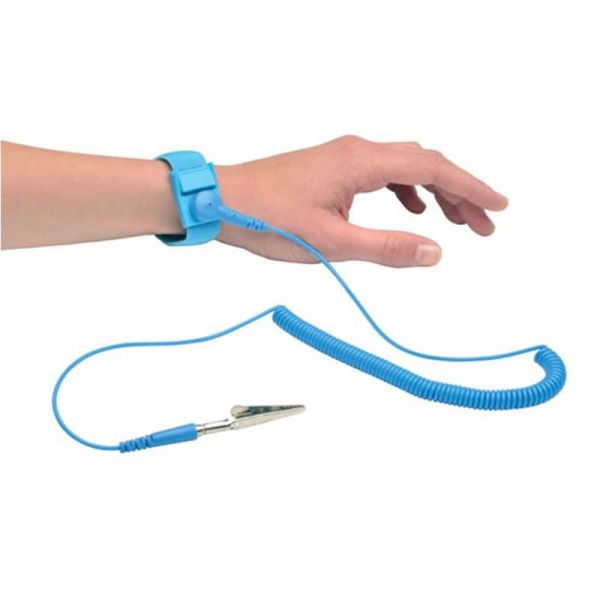
\includegraphics[width=0.35\textwidth]{esd.jpg}
	\caption{Pulsera de descarga}
\end{figure}
También es importante que manipulemos la máquina una vez que lleve un tiempo desenchufada. De esta forma, los condensadores se descargarán.

\subsection{Fuente de alimentación}
Se encarga de convertir la corriente alterna en continua.
\begin{itemize}
	\item Entrada: AC (220V-50Hz)
	\item Salida: DC($\pm$5V, $\pm$12V, $\pm$3.3V)
\end{itemize}
La fuente de alimentación (\textit{PSU, \textbf{P}ower \textbf{S}upply \textbf{U}nit}) alimenta tanto la placa base como los periféricos. Su factor más importante es la potencia que entrega (250W, 500W...)
\begin{figure}[H]
	\centering
	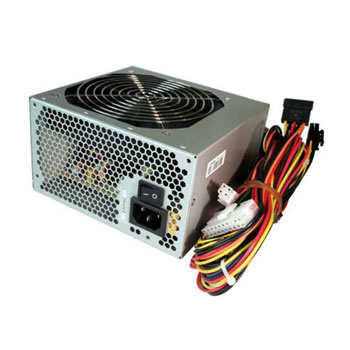
\includegraphics[width=0.35\textwidth]{psu.jpg}
	\caption{Fuente de alimentación}
\end{figure}

El voltaje $+5$V se utiliza normalmente cuando la máquina está en \textit{standby} para funciones como \textit{Wake On Lan} (encender cuando se solicite desde LAN).\\

Los distintos elementos de un ordenador (por ejemplo la CPU) necesitan a veces un voltaje menor (por ejemplo, 0.8V). Para ello existe el \textit{VRM, \textbf{V}oltage \textbf{R}egulation \textbf{M}odule} o módulo regulador de voltaje. Está compuesto por bovinas, condensadores y transistores y su misión es proporcionar corriente continua de distintos voltajes a los componentes y \textbf{mantenerla}, lo que aporta estabilidad. Suele colocarse cerca de los elementos que alimenta, como la CPU o la RAM. En equipos modernos se ubica bajo un disipador.

\begin{figure}[H]
	\centering
	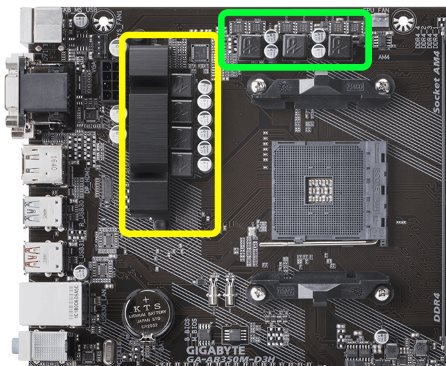
\includegraphics[width=0.35\textwidth]{vrm.jpg}
	\caption{Módulo de regulación de voltaje situado al lado del zócalo de la CPU}
\end{figure}

\begin{figure}[H]
	\centering
	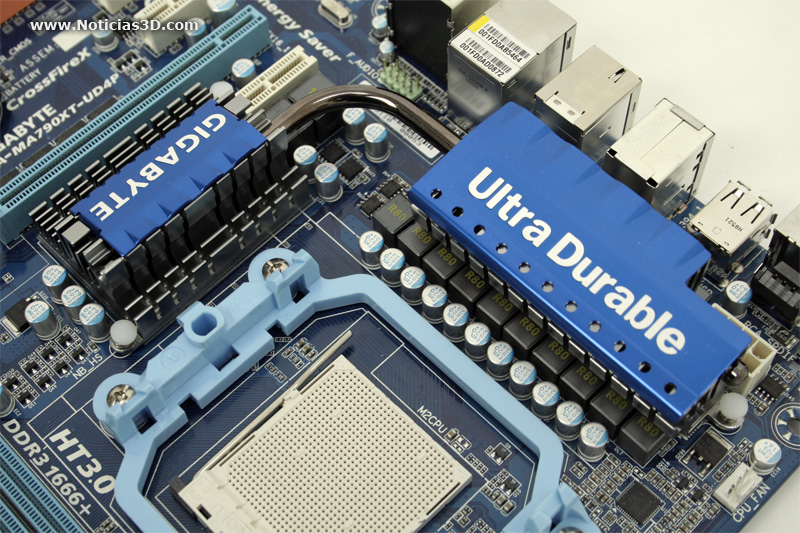
\includegraphics[width=0.35\textwidth]{vrm_disip.jpg}
	\caption{Módulo de regulación de voltaje bajo disipador}
\end{figure}

\subsection{Disipadores de calor}
Son elementos que se utilizan para bajar la temperatura de un componente. Transfieren el calor desde el componente hacia el aire. Pueden ser de dos tipos:
\begin{itemize}
	\item Pasivo (no necesita energía para funcionar).

	\item Activo (necesita energía, normalmente para un ventilador).
\end{itemize}
\begin{figure}[H]
	\centering
	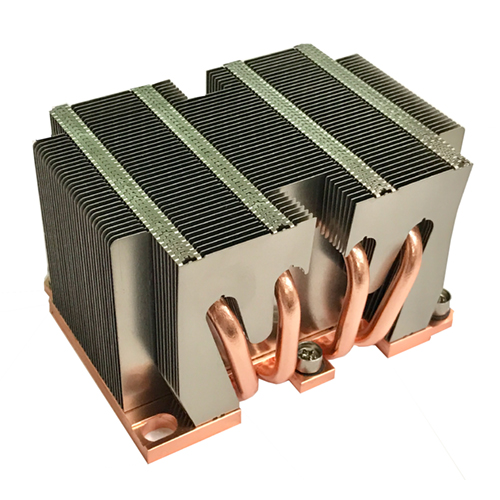
\includegraphics[width=0.25\textwidth]{passive.jpg}
	\caption{Disipador pasivo}
\end{figure}

\begin{figure}[H]
	\centering
	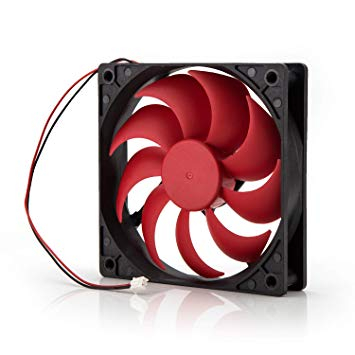
\includegraphics[width=0.25\textwidth]{fan.jpg}
	\caption{Disipador activo (ventilador de chasis)}
\end{figure}

Para refrigerar la CPU se combinan ambos tipos (a un disipador pasivo se le añade un ventilador). Este ventilador es controlado mediante un conector de 4 pines (\textit{CPU\_FAN}), que permite, además de darle energía al ventilador, controlar y medir su velocidad en cada momento.\\

Para facilitar la transferencia de calor entre la CPU y el disipador pasivo se emplea \textit{pasta térmica}.

\begin{figure}[H]
	\centering
	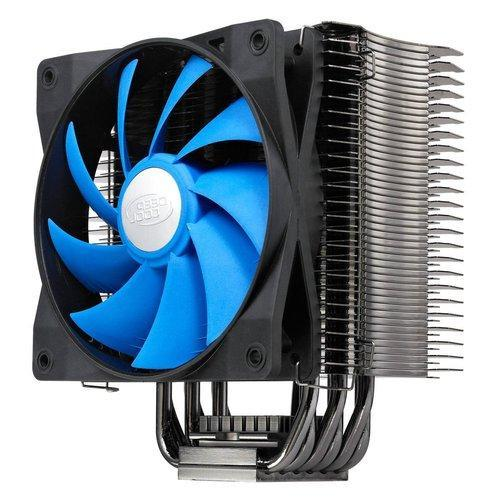
\includegraphics[width=0.25\textwidth]{cpufan.jpg}
	\caption{Disipador de CPU (combina activo y pasivo)}
\end{figure}

\begin{figure}[H]
	\centering
	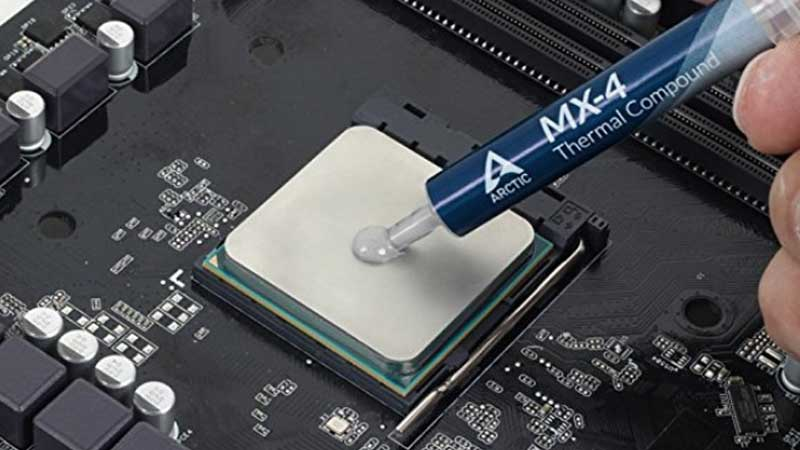
\includegraphics[width=0.25\textwidth]{thermal.jpg}
	\caption{Pasta térmica}
\end{figure}


\subsection{Zócalo de CPU (\textit{CPU Socket})}

Este elemento se encarga de conectar el microprocesador (CPU) con la placa base de forma que la CPU pueda cambiarse sin necesidad de soldaduras. Existen varios tipos de zócalo:
\begin{itemize}
	\item \textit{PGA-ZIF, \textbf{P}in \textbf{G}rid \textbf{A}rray - \textbf{Z}ero \textbf{I}nsertion \textbf{F}orce}. La placa tiene agujeros en los que entran los pines de la CPU. Se utiliza una palanca para fijar la CPU al zócalo.
	\item \textit{LGA, \textbf{L}and \textbf{G}rid \textbf{A}rray}. La CPU tiene contactos y la placa base una matriz de superficies conductoras, de forma que así los pines no pueden doblarse. La CPU se asegura mediante una placa de metal.
\end{itemize}

\begin{figure}[H]
	\centering
	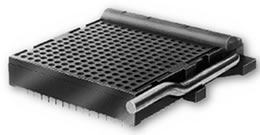
\includegraphics[width=0.25\textwidth]{pgazif.jpg}
	\caption{Socket \textit{PGA-ZIF}}
\end{figure}
\begin{figure}[H]
	\centering
	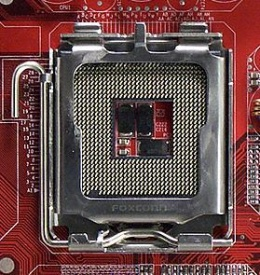
\includegraphics[width=0.25\textwidth]{lga.jpeg}
	\caption{Socket \textit{LGA}}
\end{figure}


\subsubsection{Historia de las CPU}
\begin{itemize}
	\item La litografía de las CPUs (tamaño de los transistores) ha ido descendiendo exponencialmente, lo que hace que se puedan incorporar más transistores.
	\item El número de transistores ha ido creciendo exponencialmente, lo que hace que crezca el rendimiento.
	\item Surge la Ley de Moore: cada dos años se duplica el número de transistores de un procesador.
	\item La frecuencia de reloj subía exponencialmente, al igual que el consumo.
	\item En 2005 se llegó a la barrera térmica (más calor haría que el chip se quemase). La frecuencia a la que se llegó fue de unos 4.2Ghz.
	\item La competitividad se centra actualmente en fabricar CPUs con más caché, más núcleos, controlador gráfico integrado, etc. (la lucha por la máxima frecuencia terminó).
\end{itemize}

\begin{figure}[H]
	\centering
	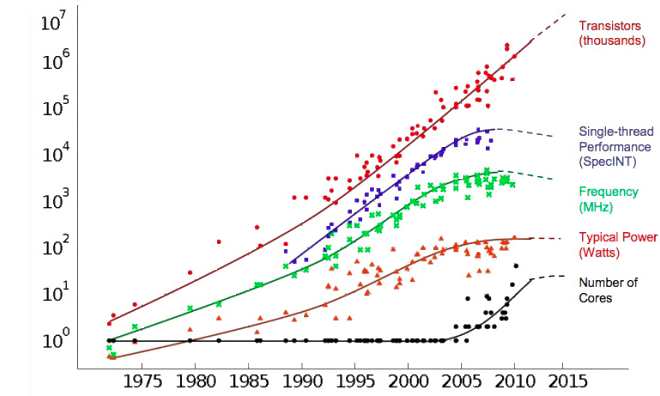
\includegraphics[width=0.5\textwidth]{cpuhistory.png}
	\caption{Evolución histórica de las CPU}
\end{figure}

Hoy día los principales fabricantes de CPU son IBM, Intel y AMD.

\subsubsection{Intel Xeon}

Son la división de procesadores Intel específica para servidores. Incorporan más soporte para multiprocesamiento, más tecnologías (como \textit{HyperThreading}, capaz de realizar la emulación de dos hebras mediante un único núcleo) y, en general, mayores prestaciones que las de un equipo sobremesa.\\

Una CPU para servidores es capaz de coexistir con otra CPU en la misma placa. Sin embargo, esto acarrea un problema: si una CPU quiere acceder a un banco de memoria de la otra, necesita pasar por la otra CPU de forma muy rápida. Para solucionar esto surgen los \textit{UPI Link}, conexiones muy rápidas entre las CPUs. Cuantos más \textit{UPI Links} tenga una CPU, mayor velocidad de acceso tendrá.

\begin{figure}[H]
	\centering
	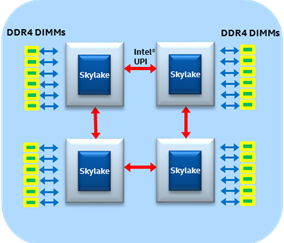
\includegraphics[width=0.5\textwidth]{upi.png}
	\caption{Esquema de funcionamiento de los \textit{UPI Links} (flechas rojas)}
\end{figure}

Estos procesadores suelen soportar memoria ECC (\textit{Error Correcting Code}). Estas memorias incorporan un chip más (8 bits de redundancia para detectar si hay un error y corregirlo).

\subsubsection{AMD (EPYC y Opteron)}

Son los procesadores de AMD dedicados para servidores. El primer Opteron (presentado en 2003) fue el primer procesador que utilizaba el conjunto de instrucciones AMD x86-64. Por ser AMD la primera marca en lanzar un procesador x86-64, hoy día las distribuciones de 64 bits se siguen llamando AMD64.\\

Actualmente hay tres grandes familias de CPUs AMD para servidores:
\begin{itemize}
	\item EPYC.
	\item Opteron X-Series (basada en APU, \textit{Accelerated Processing Unit}). Incorporan CPU y GPU en un mismo chip, además de E/S (son un SoC, \textit{System on a Chip}). Intel también incorpora una GPU en muchos de sus procesadores. Usan la arquitectura x86
	\item Opteron A-Series. Utilizan el repertorio ARM. Tienen un gran ratio prestaciones/consumo y son SoC con controladores PCI-e, Ethernet y SATA en el propio chip. Consumen menos de 30W.
\end{itemize}

\subsubsection{IBM Power (\textit{Performance Optimization With Enhanced RISC})}

IBM fabrica grandes máquinas con muchas E/S. Esto aporta gran fiabilidad y redundancia.\\

El procesador más destacado es el \textbf{IBM Power 9}. Sus características más importantes son que la memoria caché L3 es distribuida y que cada núcleo puede ejecutar hasta 8 hilos.

\subsection{Ranuras para la memoria DRAM (\textit{Dynamic Random Access Memory})}

Son los conectores donde se insertan los módulos de memoria principal, que tiene una velocidad inferior a la SRAM (caché) pero mayor densidad.\\

La DRAM tiene las siguientes características:
\begin{itemize}
	\item Se comunica con la CPU mediante un bus de 64 bits.
	\item RW: lectura y escritura.
	\item Volátil: al apagar la máquina se elimina su contenido.
	\item Necesita refresco: la información se desvanece si no se leen y reescriben los datos cada X tiempo. De esto se encarga un controlador dedicado.
	\item Tiene una mayor densidad, ya que cada celda es mucho más simple.
\end{itemize}
\begin{figure}[H]
	\centering
	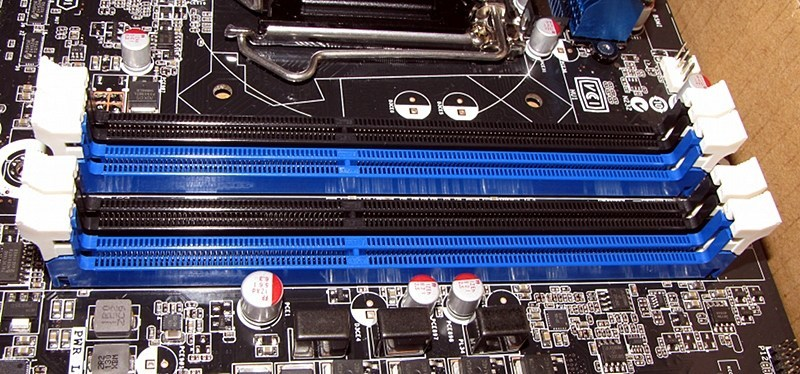
\includegraphics[width=0.5\textwidth]{ramslot.jpg}
	\caption{Slot para memoria RAM}
\end{figure}
\begin{figure}[H]
	\centering
	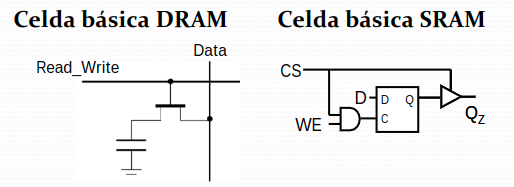
\includegraphics[width=0.5\textwidth]{ramcells.png}
	\caption{Celdas DRAM y SRAM}
\end{figure}

\subsubsection{Evolución histórica de la DRAM}
\begin{itemize}
	\item Se comienza con la \textbf{SDRAM}: Synchronous DRAM. Hay una señal de reloj para saber cuándo se podrá obtener el dato.
	\item Tras las memorias síncronas, la competitividad se centra en obtener más datos por cada ciclo de reloj (DDR: 2 datos, DDR2, 4 datos, ..., DDR4: 8 datos).
	\item Con el paso del tiempo el número de conectores de cada módulo ha ido aumentando.
	\item El voltaje ha ido descendiendo con los años (lo que acarrea un menor consumo).
	\item Desde DDR2 el bus de datos se ha estancado en 64 bits. Cada vez que la CPU pide un dato, se le mandan 64 bits. El bus se usa para lectura y escritura a la vez, por lo que no se pueden realizar las dos operaciones al mismo tiempo (\textit{half-duplex}).
	\item El ancho de banda (\textit{throughput}, productividad) ha ido aumentando con los años.
\end{itemize}

Los tipos de memorias RAM son los siguientes:

\begin{itemize}
	\item \textit{SIPP: \textbf{S}inge \textbf{I}n-line \textbf{P}in \textbf{P}ackage}.
	\item \textit{SIMM: \textbf{S}inge \textbf{I}n-line \textbf{M}emory \textbf{M}odule}.
	\item \textit{DIMM: \textbf{D}ual \textbf{I}n-line \textbf{M}emory \textbf{M}odule}.
\end{itemize}

\begin{figure}[H]
	\centering
	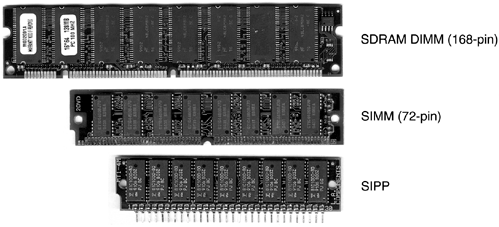
\includegraphics[width=0.7\textwidth]{ramtypes.png}
	\caption{Tipos de RAM}
\end{figure}

\subsubsection{Tipos de memoria DIMM}

\begin{itemize}
	\item DIMM o U-DIMM (\textit{Unbuffered DIMM}). No tienen registro (buffer). Son las que se utilizan en los PC.
	\item EU-DIMM: son U-DIMM con ECC.
	\item R-DIMM (\textit{Registered DIMM}). Hay un registro que almacena las señales de control, por lo que los módulos pueden tener mayor capacidad. Como consecuencia la latencia es mayor, ya que hay que acceder al registro antes que a la celda. Tienen ECC.
	\item LR-DIMM (\textit{Load Reduced DIMM}). El registro almacena tanto las señales de control como el dato a manejar. Por tanto, son las que admiten más memoria. Son también las más caras. Tienen ECC.
	\item SO-DIMM (\textit{Small Outline DIMM}). Son más pequeñas, ya que se utilizan en portátiles (tienen menos contactos).
\end{itemize}

\subsubsection{Canales y bancos de memoria DRAM}

Un banco de memoria es un grupo de módulos que comparten canal de memoria. No se puede acceder en paralelo a dos módulos bajo un mismo banco, pero sí a distintos bancos.\\

Los canales unen los bancos con la CPU.

\begin{figure}[H]
	\centering
	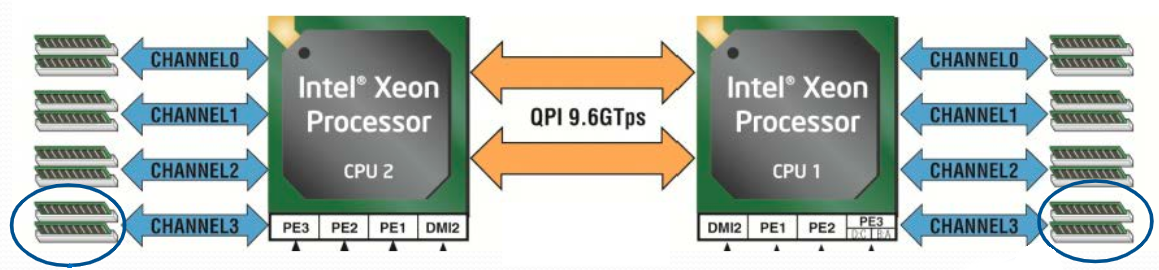
\includegraphics[width=0.7\textwidth]{rambanks.png}
	\caption{Canales (flechas) y bancos (rodeados) de RAM}
\end{figure}

\subsubsection{Rangos de memoria DRAM}

Los rangos son agrupaciones de memoria que suman una palabra completa (64 bits o 72 si la memoria tiene ECC). La notación utilizada es la siguiente:
\begin{itemize}
	\item 1Rx4: módulo de un rango con chips de 4 bits ($\frac{64}{4}= 16$ chips por rango).
	\item 2Rx8: módulo de dos rangos con chips de 8 bits ($\frac{64}{8}= 8$ chips por rango). Por ejemplo, un módulo con dos caras, cada una con un rango de 8 chips de 8 bits cada uno.
\end{itemize}

Algunas CPUs pueden no soportar un determinado número de rangos.

\begin{figure}[H]
	\centering
	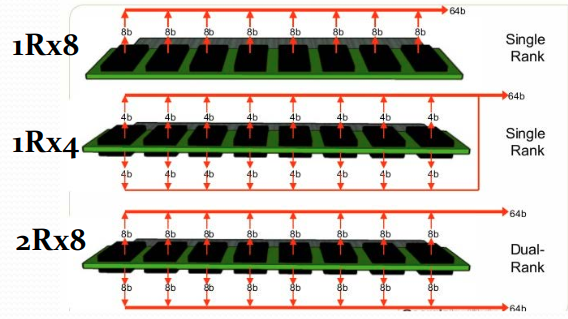
\includegraphics[width=0.7\textwidth]{ramranks.png}
	\caption{Notación de rangos de RAM}
\end{figure}

En las especificaciones de una memoria DRAM suelen aparecer los siguientes campos:
\begin{itemize}
	\item DDR4-\textbf{2666}. Es la frecuencia efectiva. El módulo puede realizar 2666 MegaTransferencias por segundo. Como cada transferencia es de 64 bits (8 bytes): $2666 MTps * 8 B= 21328Mbps \approx$ 21300.
	\item DDR4-PC4-\textbf{21300}. Viene del apartado anterior.
	\item CL19. Latencia de acceso de 19 ciclos de reloj. Hemos de tener cuidado, ya que la velocidad depende tanto de la latencia como de la frecuencia.
	\item \textit{x4 based}. Cada chip aporta 4 bits (por tanto, si la memoria tiene ECC, hay $\frac{72}{4}=18$ módulos en cada cara).
	\item \textit{Dual Ranked}. En la otra cara hay otros 18 módulos.
\end{itemize}

\subsection{Ranuras de expansión}

Sireven para extender la funcionalidad de la placa base mediante otras tarjetas PCB. Los principales slots son:
\begin{itemize}
	\item \textbf{ISA} (\textit{\textbf{I}ndustry \textbf{S}tandard \textbf{A}rchitecture}). Usaban un bus de 16 bits en half-dúplex (el mismo bus se usaba para lectura y escritura).
	\item \textbf{PCI} (\textit{\textbf{P}eripheral \textbf{C}omponent \textbf{I}nterconnect}). Fueron lanzadas por Intel. Sus principales características son:
		\begin{itemize}
			\item \textit{Plug\&Play}: la tarjeta se conecta a la máquina y ya se puede usar. No se necesita especificar la interrupción con la que la máquina puede comunicarse con la tarjeta (en ISA sí).
			\item Se usa un bus paralelo (half-dúplex) de 32 ó 64 bits. La señal de reloj es igual para los 32 ó 64 bits.
			\item Existe una versión específica para servidores (PCI-X) que lograba un ancho de banda de prácticamente el doble.
		\end{itemize}
		\item \textbf{AGP} (\textit{\textbf{A}ccelerated \textbf{G}raphics \textbf{P}ort}). Desarrolladas por Intel. Es una conexión específica para GPUs, por lo que se eliminan características de PCI que utilizaban el resto de tarjetas.
		\item \textbf{PCIe} (\textit{PCI Express}). Es loa interfaz utilizada actualmente.
		\begin{itemize}
			\item Se usa una conexión en serie punto a punto (las líneas no son compartidas) por medio de \textit{LANES}.
			\item Cada \textit{LANE} está compuesta por 4 cables: dos para leer y 2 para escribir (full-dúplex) .
			\item Cada \textit{LANE} tiene su propia señal de reloj (incrustada en los datos que transfiere).
			\item \textit{Hot plug}, es decir, podemos conectar la tarjeta a la máquina sin apagarla, ya que el número de \textit{LANES} se negocia automáticamente.
			\item Se virtualiza la E/S (el hipervisor de una máquina virtual no tiene que gestionar el acceso al recurso, sino que la tarjeta reserva una parte para la MV	item).
			\item La escalabilidad es muy sencilla, sólo hay que incrementar el número de \textit{LANES}.
			\item Se añade redundancia, por lo que las codificaciones más comunes son 8b/10b (el dato ocupa 8 bits pero se añaden 2 más de redundancia) y 128b/130b.
			\item Las versiones de PCIe y sus respectivas velocidades (en cada línea y sentido) son las siguientes:
			\begin{itemize}
				\item PCIe 1.1: 2.5GT/s (250MB/s). En la codificación 8b/10b dividimos las gigatransferencias entre 10 para hallar la velocidad en MB/s.
				\item PCIe 2.0: 5GT/s (500/s)
				\item PCIe 3.0: 8GT/s (en torno a 1GB/s). Aquí se comenzó a usar la codificación 128b/130b, por lo que dividimos entre 8.
				\item PCIe 4.0: 16GT/s (en torno a 2GB/s)
			\end{itemize}
			\item El número de \textit{LANES} habitual es x1,x2,x4,x8 o x16 (tarjetas gráficas).
			\item Las principales ventajas de utilizar un protocolo de serie con respecto a uno paralelo son el aumento de frecuencia de reloj (lo que evita el \textit{timing skew}, fenómeno por el que una señal de reloj llega a distintos componentes en tiempos distintos debido a que la longitud del cable es distinta) y una mayor escalabilidad.
		\end{itemize}
\end{itemize}

\begin{figure}[H]
	\centering
	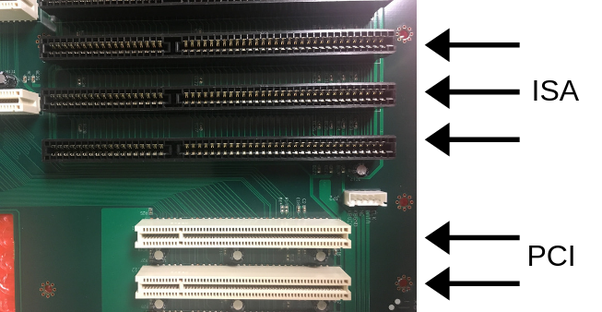
\includegraphics[width=0.75\textwidth]{isapci.png}
	\caption{Slots ISA y PCI}
\end{figure}

\begin{figure}[H]
	\centering
	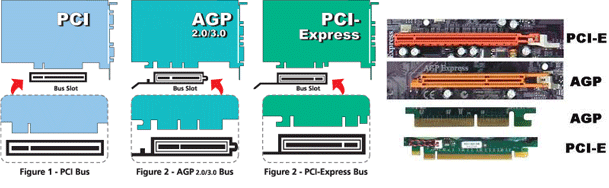
\includegraphics[width=\textwidth]{pcieagp.png}
	\caption{Slots PCI, AGP y PCI Express}
\end{figure}

\begin{figure}[H]
	\centering
	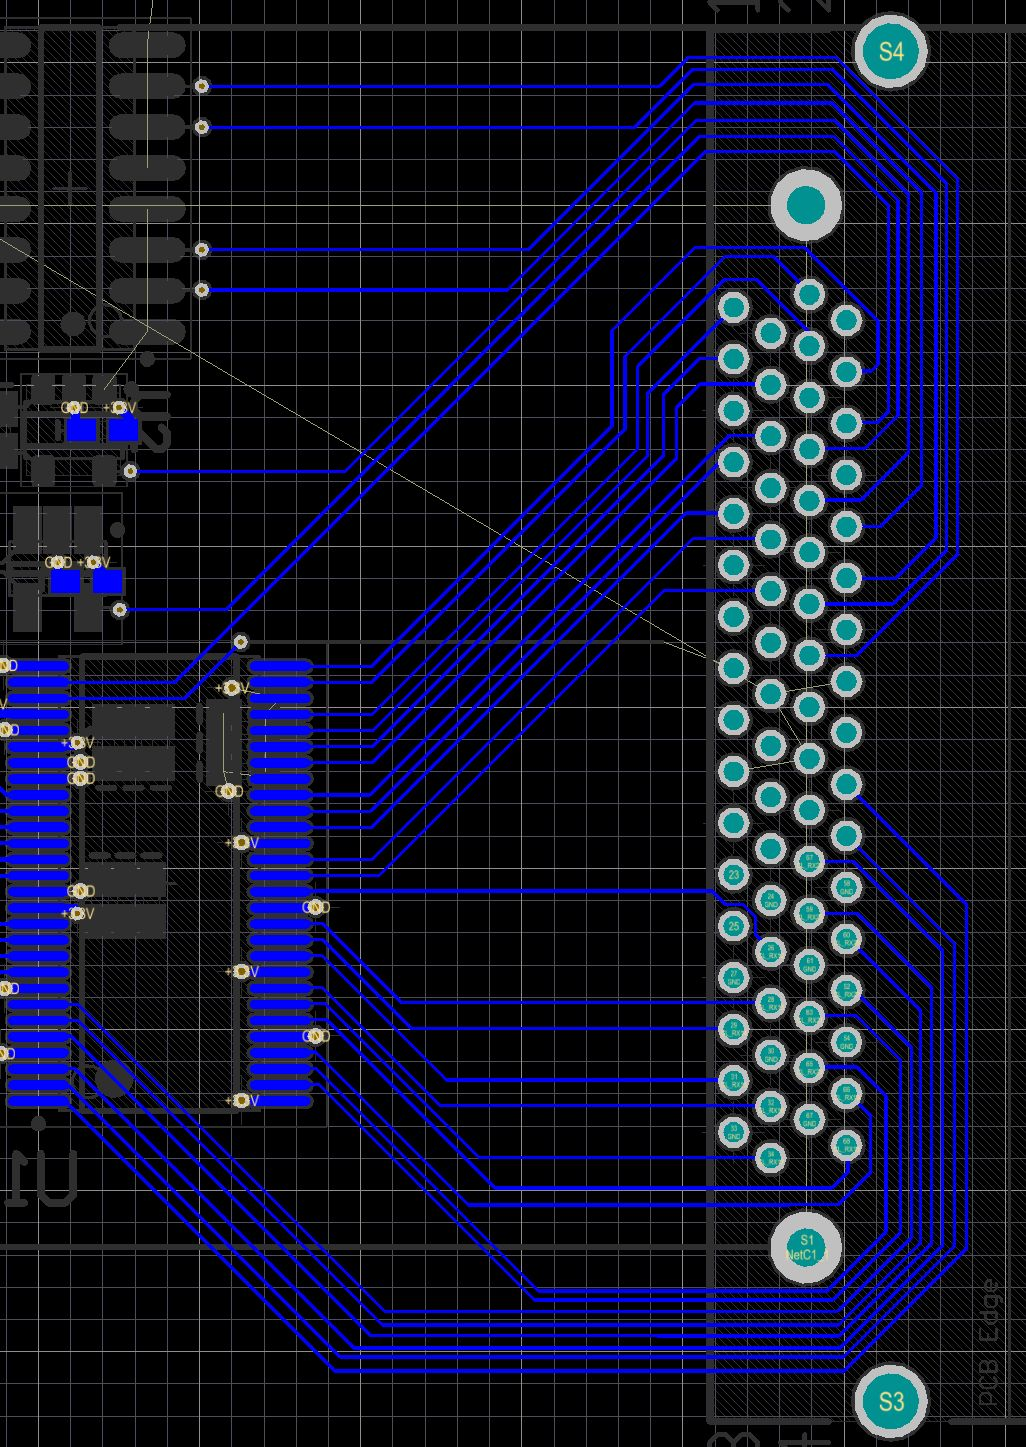
\includegraphics[angle=90,width=0.5\textwidth]{timskew.jpg}
	\caption{Las líneas no tienen la misma longitud, lo que provoca el \textit{timing skew}}
\end{figure}

\subsection{Almacenamiento permanente (no volátil)}

Estos dispositivos sirven para almacenar información sin que se pierda al apagar la máquina. Se dividen en :
\begin{itemize}
	\item Según su tipo:
	\begin{itemize}
		\item Magnéticos (disquetes, HDD, cintas).
		\item Ópticos (CD, DVD, Blu-Ray).
		\item Memoria Flash (SSD).
	\end{itemize}
	\item Según su factor de forma (en pulgadas): 3.5, 2.5 y 1.8.
	\item Según su conexión a la placa base: ATA (IDE), SATA, M.2, SCSI, SAS, etc,
\end{itemize}

\subsubsection{Discos duros (HDD)}
\begin{itemize}
	\item Son discos recubiertos de un material magnético. La lectura y escritura se realiza mediante un cabezal magnético móvil.
	\item Los datos se distribuyen en pistas.
	\item Las pistas se dividen en sectores, que se agrupan en clústers lógicos.
	\item Si incrementamos las revoluciones por minuto (normalmente 5400, 7200 o 10000), aumentamos la productividad y el ancho de banda.
	\item La latencia es variable: depende de dónde se encuentre el cabezal y dónde el dato.
	\item Se suele añadir un módulo de caché para acelerar la lectura.
\end{itemize}

\begin{figure}[H]
	\centering
	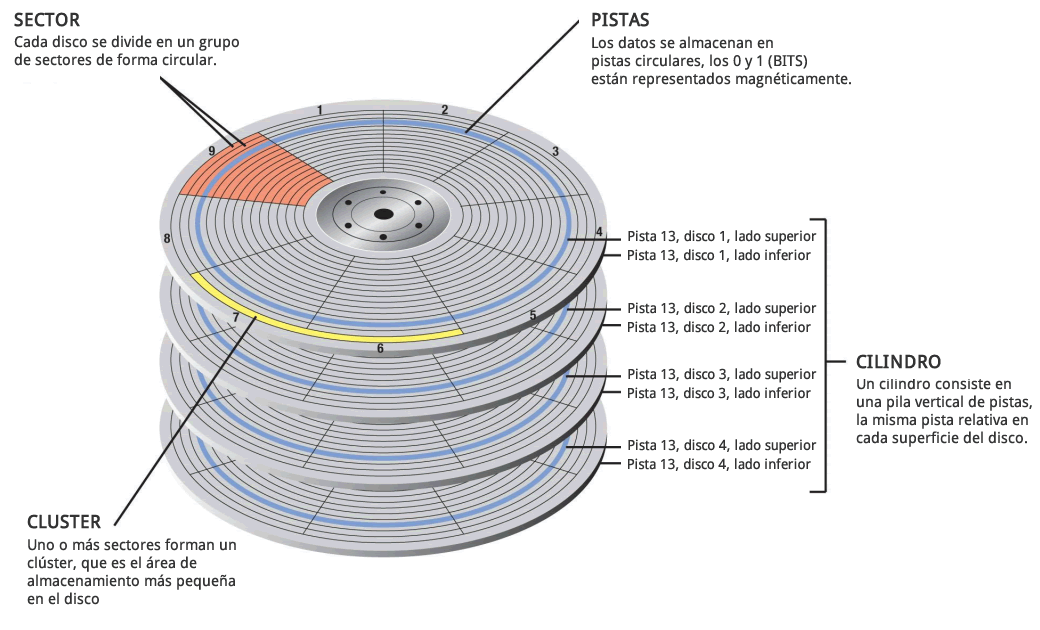
\includegraphics[width=0.75\textwidth]{hddparts.png}
	\caption{Pistas, sectores, clústers y cilindros en un HDD}
\end{figure}

\subsubsection{Unidades de estado sólido (SSD)}
\begin{itemize}
	\item Están basadas en MOSFETs de puerta flotante.
	\item Se obtiene la misma latencia accediendo a cualquier dato.
	\item La densidad de chips es más baja, por lo que la capacidad también.
	\item Las celdas más comunes son MLC (\textit{\textbf{M}ulti \textbf{L}evel \textbf{C}ell}) que admiten más de dos estados. Por ejemplo: descargado, poco cargado, muy cargado y completamente cargado.
	\item Un controlador se encarga de distribuir la información entre las celdas para equilibrar el número de escrituras (\textit{wear leveling}) y así prolongar la vida útil de la unidad.
\end{itemize}

\begin{figure}[H]
	\centering
	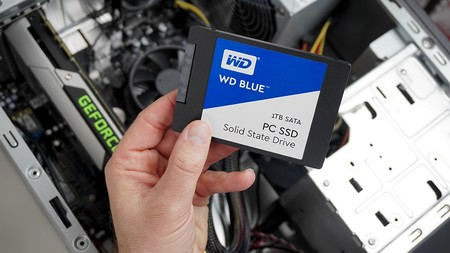
\includegraphics[width=0.5\textwidth]{ssd.jpg}
	\caption{SSD}
\end{figure}

\begin{figure}[H]
	\centering
	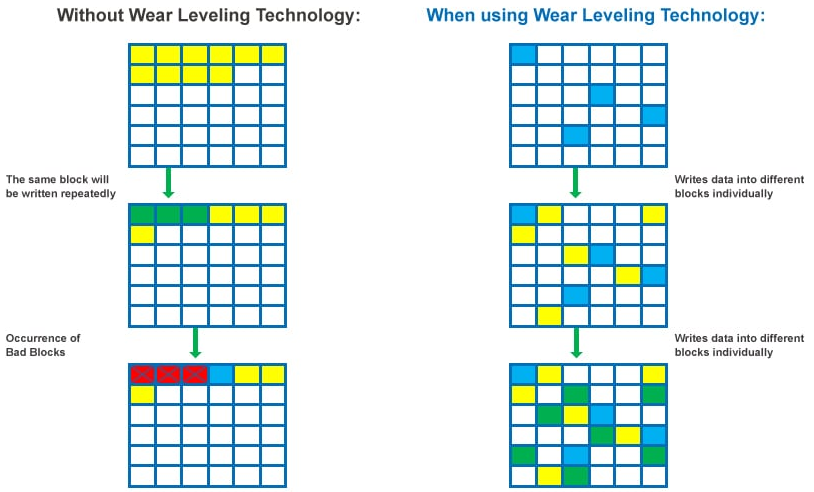
\includegraphics[width=\textwidth]{wearleveling.png}
	\caption{La importancia de \textit{wear leveling}}
\end{figure}

\subsubsection{RAID}
Consiste en combinar distintas unidades de almacenamiento para generar unidades lógicas con mayor tolerancia a fallos, fiabilidad y ancho de banda. Puede estar creado por software o por hardware (una tarjeta específica).

\subsubsection{Unidades ópticas}
Almacenan información de forma permanente a partir de surcos en un disco que se pueden leer mediante un haz de luz láser. Su principal problema es que no tienen un gran ancho de banda. Los más comunes son el CD, DVD y Blu-Ray.

\begin{figure}[H]
	\centering
	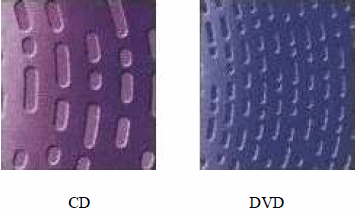
\includegraphics[width=0.5\textwidth]{surcos.png}
	\caption{Surcos en un CD y un DVD}
\end{figure}

\subsubsection{Unidades de cinta}

\begin{itemize}
	\item Almacenan información a través de una cinta recubierta de material magnético que se enrolla en carretes.
	\item La latencia suele ser alta ya que hay que rebobinar la cinta para que el cabezal lea lo adecuado.
	\item Es el medio con mayor densidad de bits (decenas de TB por cinta).
	\item Es el medio de almacenamiento masivo más barato.
	\item Se utiliza normalmente como backup.
\end{itemize}

\subsubsection{Interfaz P-ATA (\textit{\textbf{P}arallel \textbf{A}dvanced \textbf{T}echnology \textbf{A}ttachment})}

\begin{itemize}
	\item Utiliza el conector IDE (\textit{\textbf{I}ntegrated \textbf{D}evice \textbf{E}lectronics}).
	\item Emplea una faja de 40 pines con un bus paralelo (half-dúplex) de 16 bits que permite conectar dos dispositivos (maestro y esclavo).
	\item Transfiere un máximo de 133Mbps.
	\item La longitud máxima de la faja es de 45cm.
\end{itemize}


\begin{figure}[H]
	\centering
	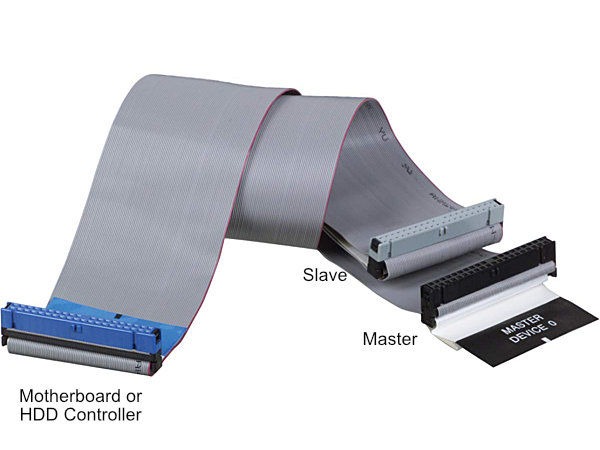
\includegraphics[width=0.5\textwidth]{patacable.jpg}
	\caption{Faja PATA}
\end{figure}

\begin{figure}[H]
	\centering
	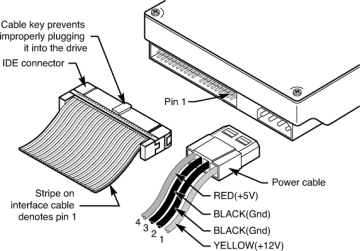
\includegraphics[width=0.5\textwidth]{pataconnection.jpg}
	\caption{Conexión de un dispositivo PATA}
\end{figure}

\subsubsection{S-ATA (\textit{\textbf{S}erial \textbf{ATA}})}
\begin{itemize}
	\item Emplea un bus serie punto a punto full-dúplex (2 cables para leer y 2 para escribir).
	\item Permite una unidad por conector.
	\item La longitud máxima del cable es de 1m.
	\item Emplea AHCI (\textit{\textbf{A}dvanced \textbf{H}ost \textbf{C}ontroller \textbf{I}nterface}), un estándar que define dos elementos:
	\begin{itemize}
		\item Hot plug: podemos conectar el disco en caliente.
		\item NCQ (\textit{\textbf{N}ative \textbf{C}ommand \textbf{Q}uery}). Aumenta el rendimiento de los discos rotacionales implementando una cola de prioridad en la que se leen los datos no según el orden de llegada de la petición, sino según su distancia a la posición actual de la aguja.
	\end{itemize}
	\item Las distintas versiones de SATA son: SATA1 (1500Mhz, 150MB/s), SATA2 (3000Mhz, 300MB/s) y SATA3 (6000Mhz, 600MB/s). Dividimos los Mhz entre 10 para obtener los MB/s.
\end{itemize}

\begin{figure}[H]
	\centering
	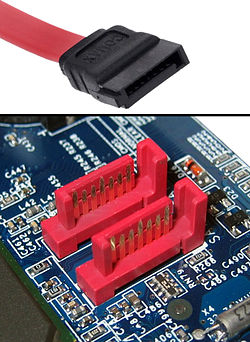
\includegraphics[width=0.3\textwidth]{sata.jpg}
	\caption{Cable y conector SATA}
\end{figure}

\begin{figure}[H]
	\centering
	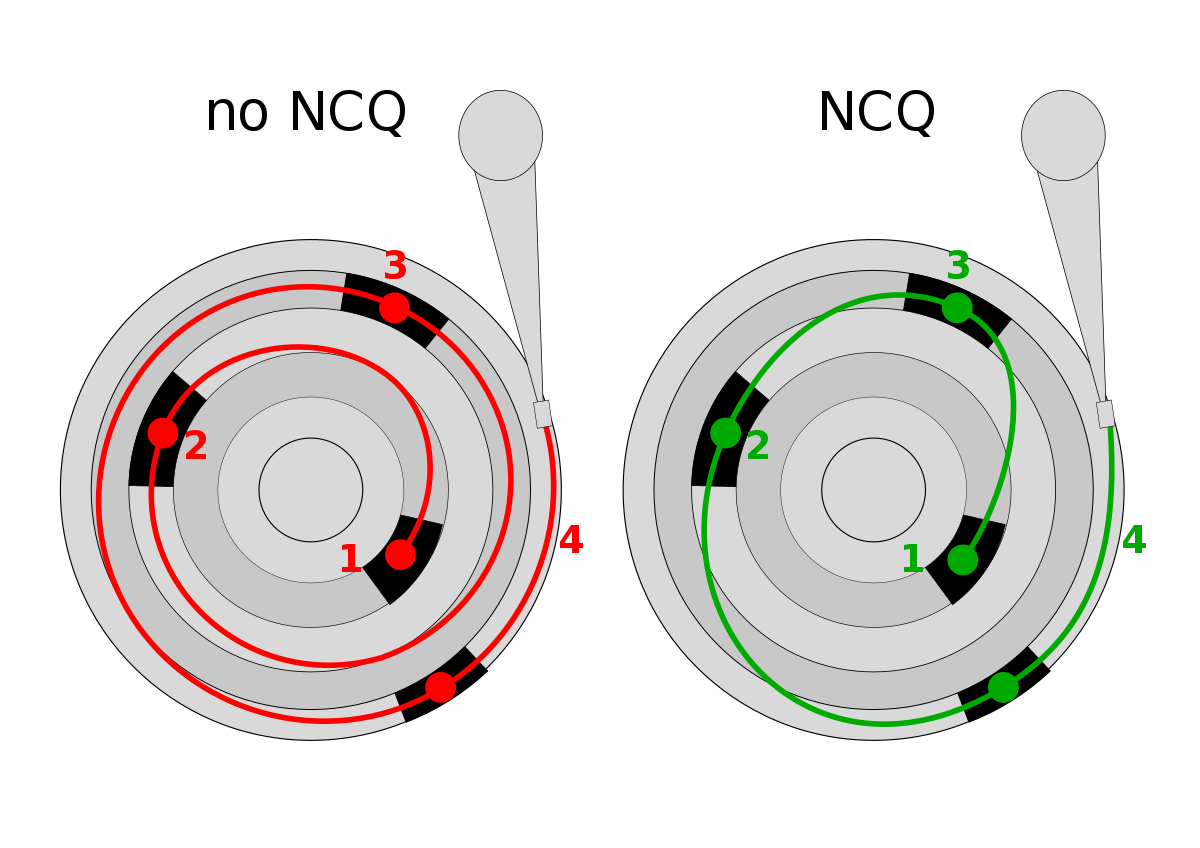
\includegraphics[width=0.5\textwidth]{ncq.png}
	\caption{Funcionamiento de NCQ}
\end{figure}

\subsubsection{SCSI y SAS}

\begin{itemize}
	\item SCSI (\textit{\textbf{S}mall \textbf{C}omputer \textbf{S}ystem \textbf{I}nterface})
	\begin{itemize}
		\item Utiliza un bus paralelo de 16 bits half-dúplex.
		\item Es más veloz que ATA.
		\item Soporta Hot Plug.
		\item Permite conectar varias unidades en cadena (\textit{daisy-chain}).
	\end{itemize}
	\item Ultra-SCSI: permite hasta 320MB/s y 12m de cable. Emplea half-dúplex también.
	\item SAS (\textit{\textbf{S}erial \textbf{A}ttached \textbf{SCSI}}). Es la versión serie de SCSI.
	\begin{itemize}
		\item Permite velocidades de hasta 12Gbps.
		\item Soporta full-dúplex.
		\item Es compatible con SATA pero usa mayores voltajes (por ello el conector de alimentación se une al de datos).
		\item Permite hasta 10 metros de cable.
		\item Se pueden conectar varias unidades al mismo puerto mediante conectores mini-SAS (4 unidades por puerto mediante un cable \textit{splitter}).
		\item También se puede emplear un expansor SAS para conectar más unidades a la placa base.
	\end{itemize}
\end{itemize}

\begin{figure}[H]
	\centering
	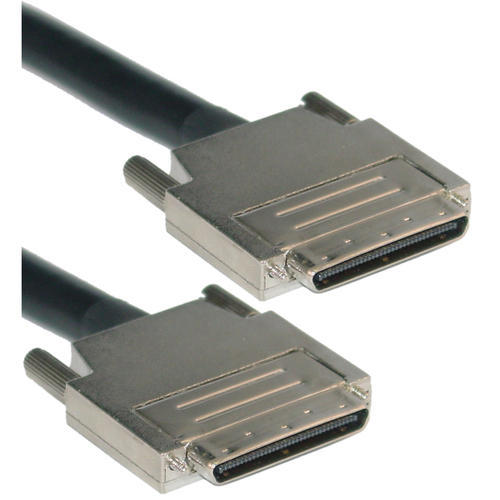
\includegraphics[width=0.3\textwidth]{scsicable.jpg}
	\caption{Cable SCSI}
\end{figure}

\begin{figure}[H]
	\centering
	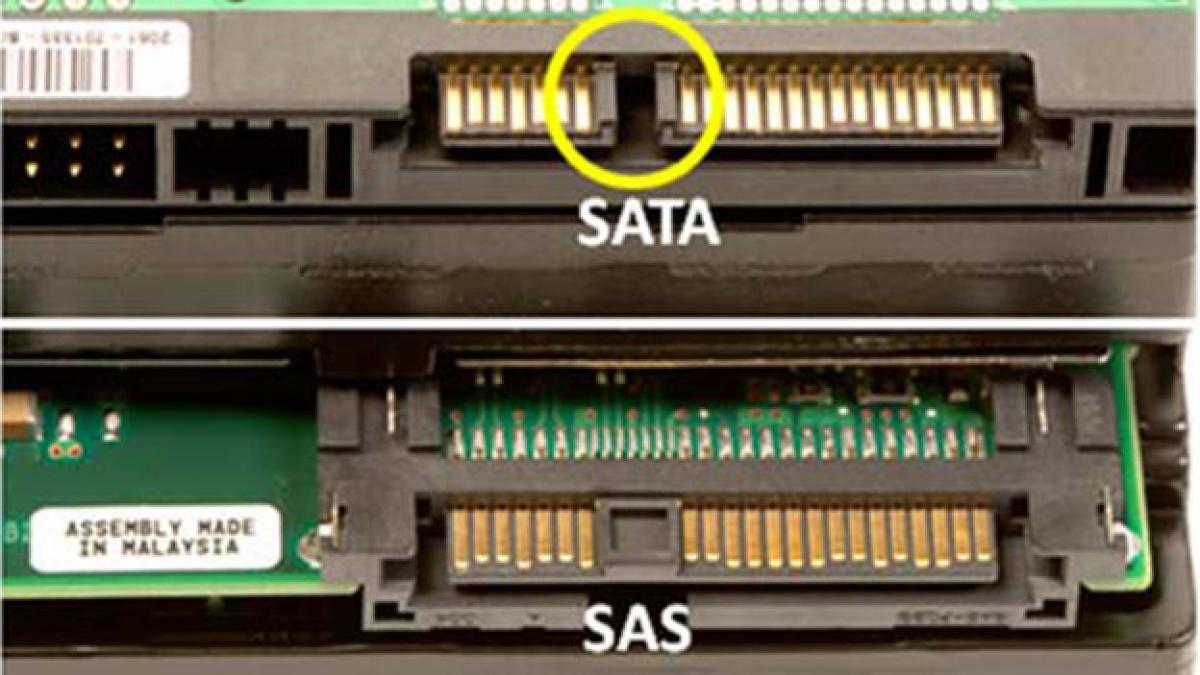
\includegraphics[width=0.5\textwidth]{sasconnector.jpg}
	\caption{Conectores SATA y SAS}
\end{figure}

\begin{figure}[H]
	\centering
	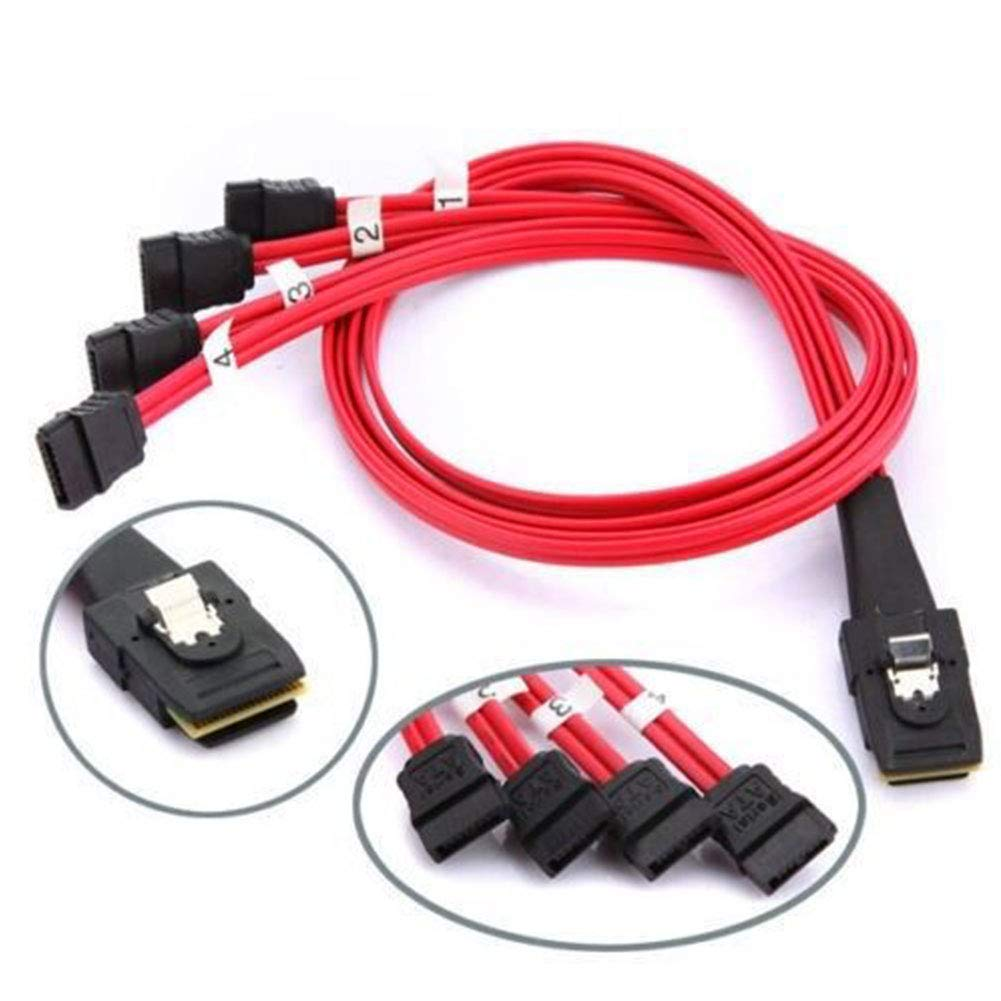
\includegraphics[width=0.35\textwidth]{sassplitter.jpg}
	\caption{Cable \textit{splitter} SAS}
\end{figure}

\begin{figure}[H]
	\centering
	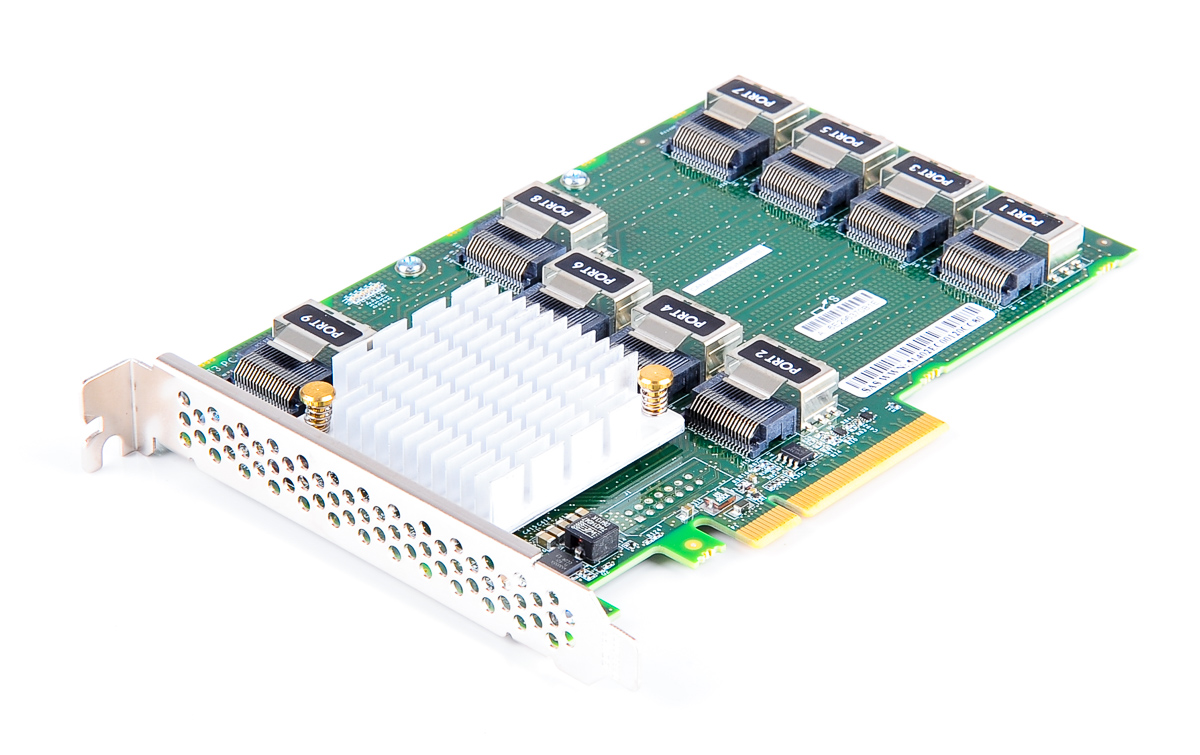
\includegraphics[width=0.35\textwidth]{sasexpander.jpg}
	\caption{Expansor SAS}
\end{figure}

\subsubsection{NVMe (\textbf{N}on \textbf{V}olatile \textbf{M}emory \textbf{E}xpress)}
Se trata de un protocolo para conectar unidades SSD mediante PCIe (normalmente x4). Su mayor ventaja es la gran escalabilidad que proporciona. Se implementan en los siguientes conectores:
\begin{itemize}
	\item PCIe x4, 4GB/s.
	\item M.2. Es el mini-sata de segunda generación. Usa internamente PCIe x4 (4GB/s).
	\item U.2. Fue lanzado por Intel. Utiliza también PCIe x4 de forma interna (4GB/s).
	\item SATA3.2. Combina PCIe y SATA, llegando a 2GB/s.
\end{itemize}

\begin{figure}[H]
	\centering
	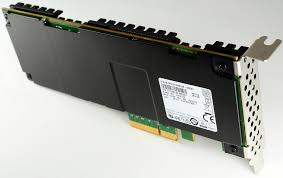
\includegraphics[width=0.35\textwidth]{pcienvme.jpeg}
	\caption{NVMe PCIe}
\end{figure}

\begin{figure}[H]
	\centering
	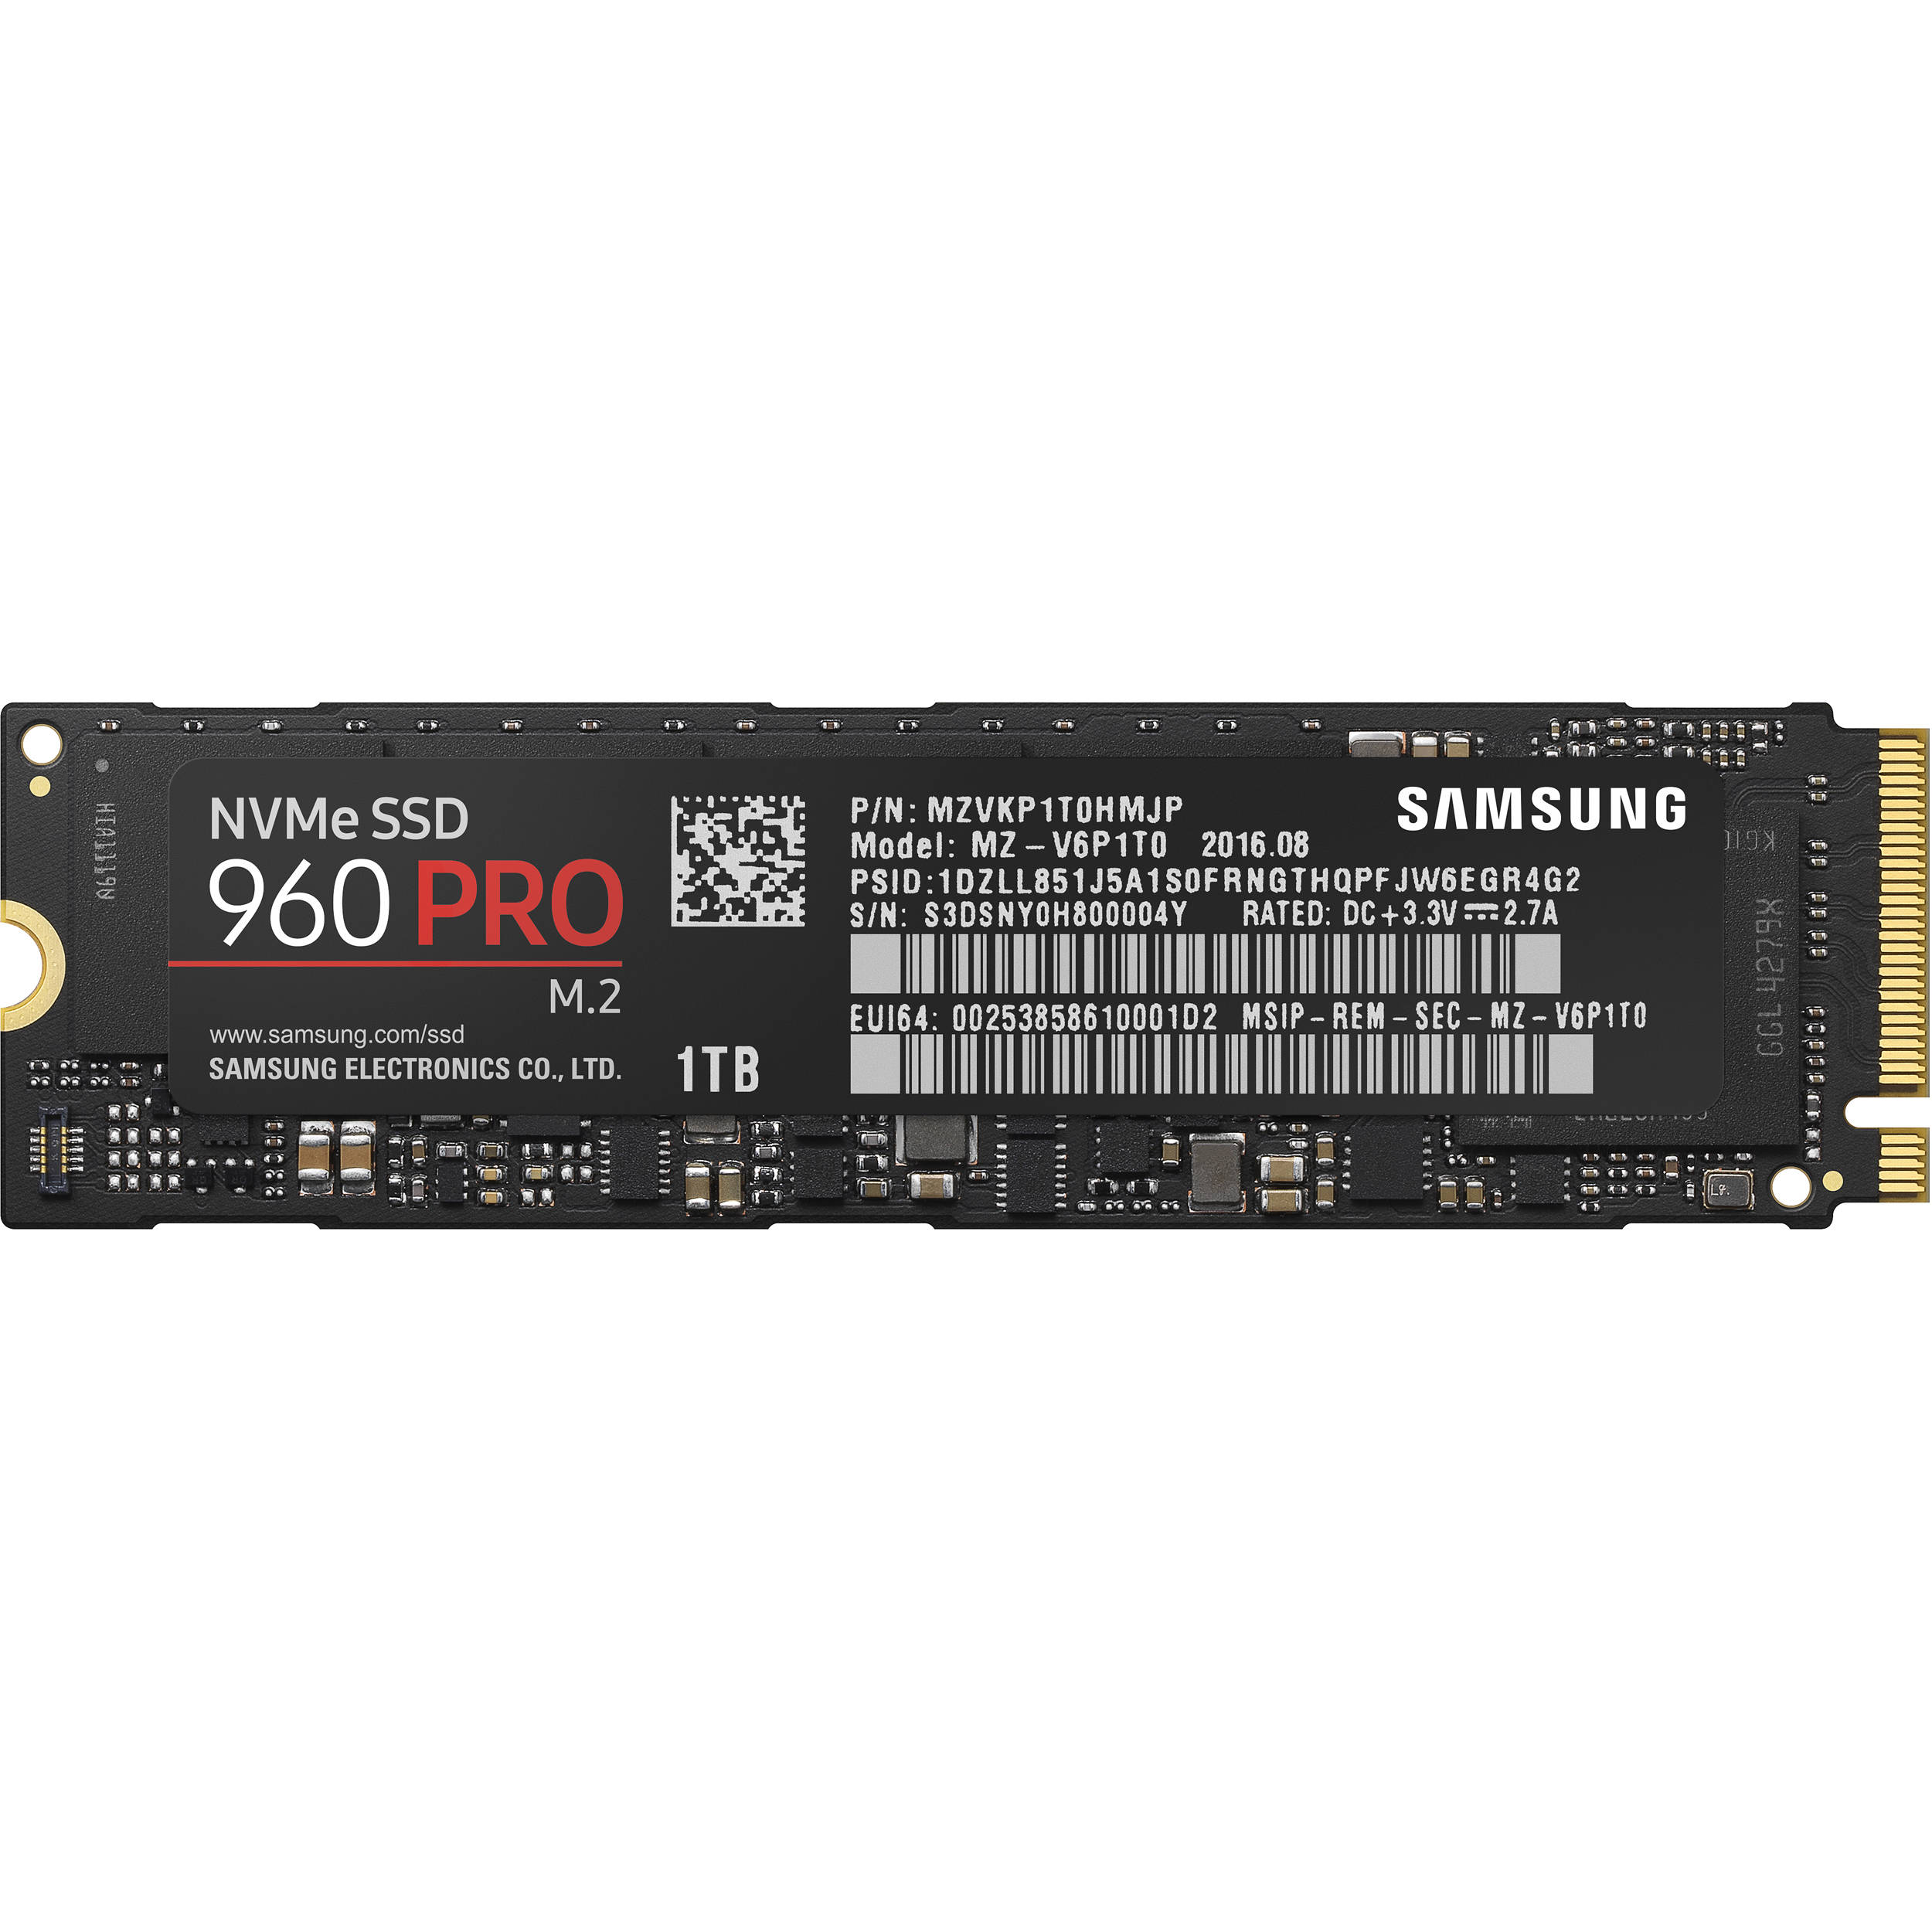
\includegraphics[width=0.35\textwidth]{m2.jpg}
	\caption{NVMe M.2}
\end{figure}

\begin{figure}[H]
	\centering
	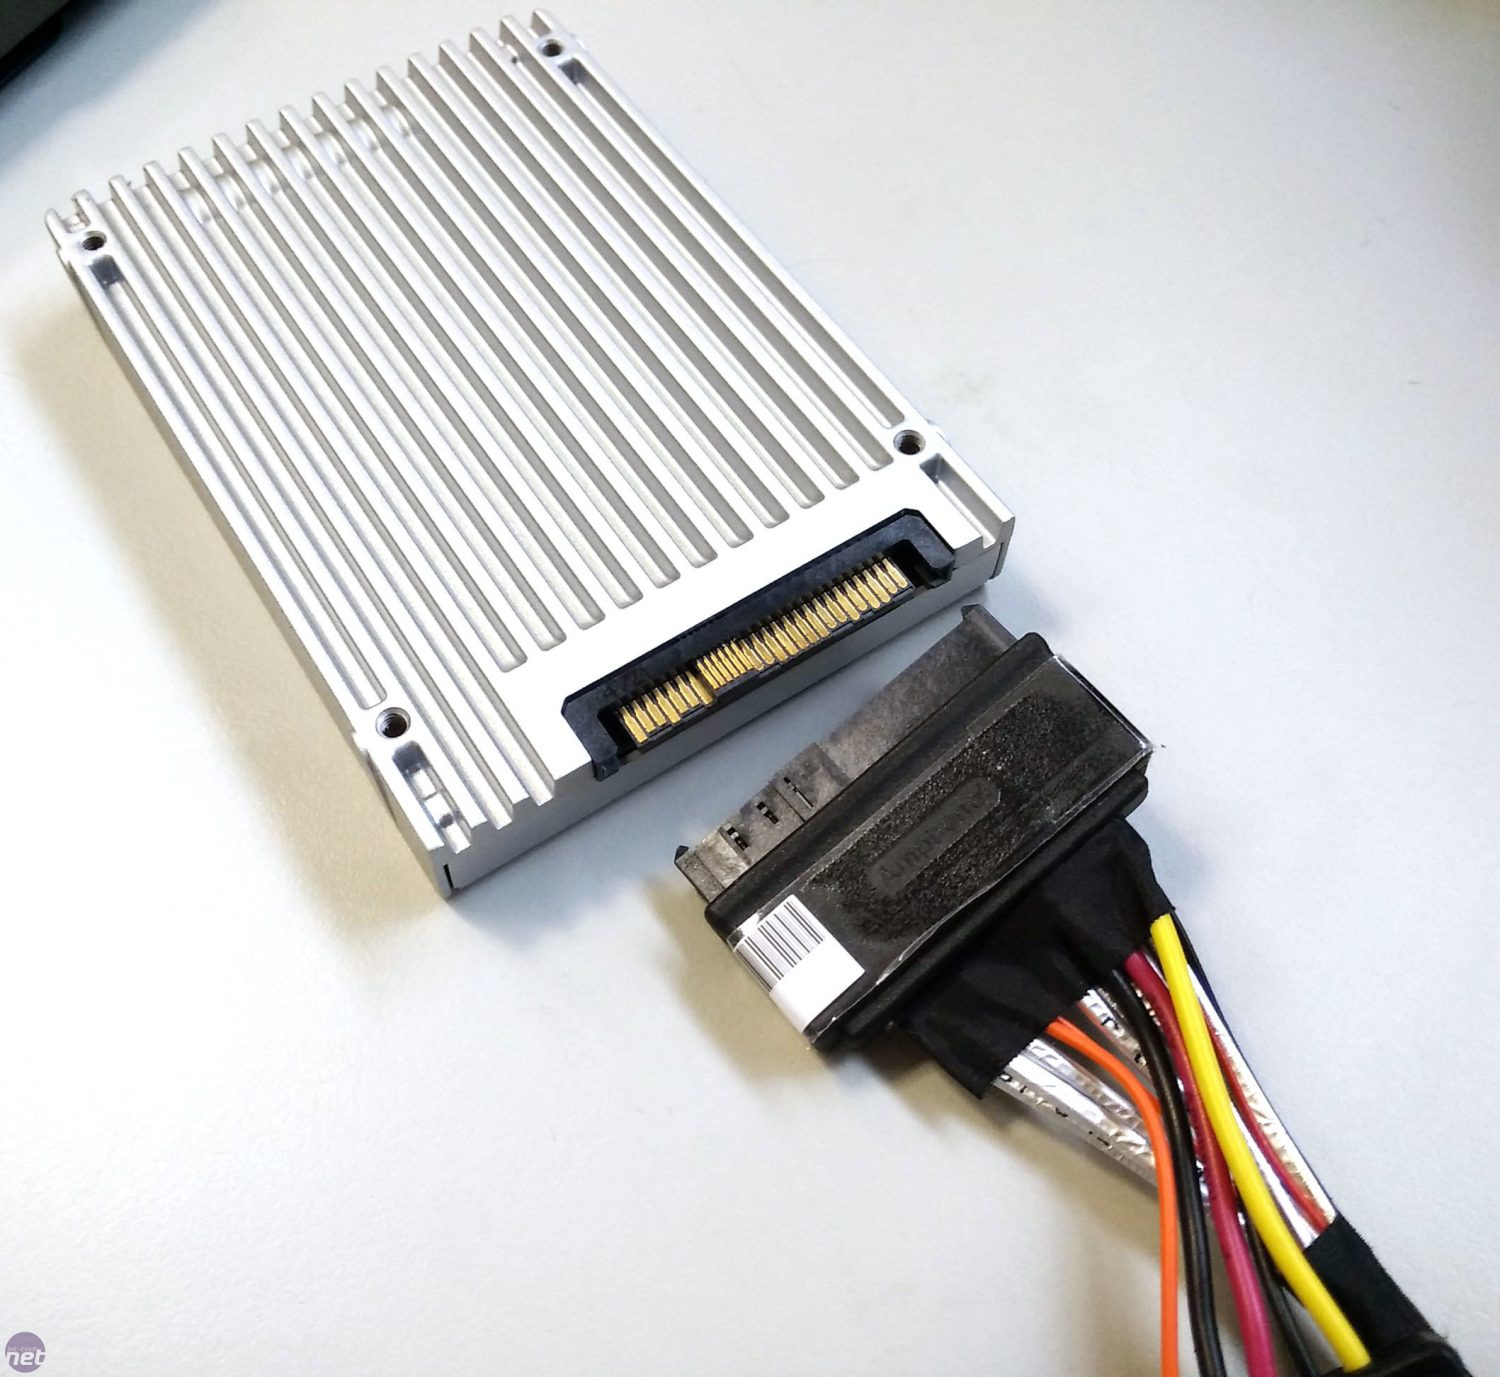
\includegraphics[width=0.35\textwidth]{u2.jpg}
	\caption{NVMe U.2}
\end{figure}

\begin{figure}[H]
	\centering
	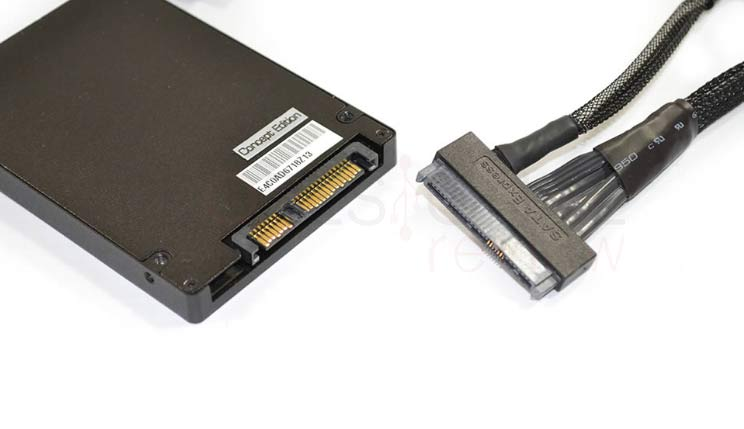
\includegraphics[width=0.35\textwidth]{satae.jpg}
	\caption{NVMe SATA Express}
\end{figure}

\subsubsection{Otras interfaces de almacenamiento}

\begin{itemize}
	\item \textbf{Fibra óptica}. Es una tecnología de red en serie constituida por dos fibras unidireccionales que transmiten en idrecciones opuestas. Permite conexión punto a punto, en anillo o redes conmutadas (muy escalable). Puede transmitir hasta distancias de kilómetros. Son utilizadas por el 90\% de las SAN.
	\item \textit{\textbf{Infiniband}}. Ofrece una comunicación en serie punto a punto de muy baja latencia entre procesadores y periféricos de alta velocidad. Se usa en redes conmutadas.
\end{itemize}

\begin{figure}[H]
	\centering
	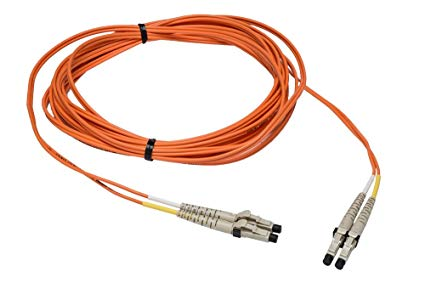
\includegraphics[width=0.35\textwidth]{fccable.jpg}
	\caption{Cable de fibra óptica}
\end{figure}

\begin{figure}[H]
	\centering
	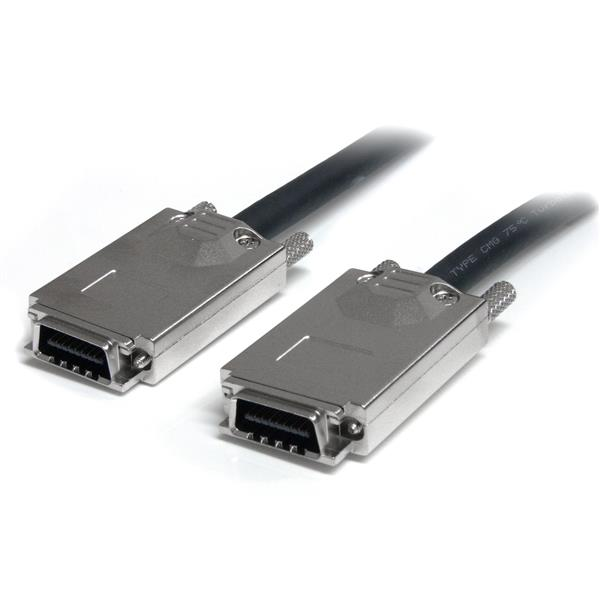
\includegraphics[width=0.35\textwidth]{infiniband.jpeg}
	\caption{Cable \textit{infiniband}}
\end{figure}

\subsection{Conectores del panel trasero}

Una placa base para servidor tiene en su panel trasero, básicamente:

\begin{itemize}
	\item Una salida de vídeo básica (normalmente VGA).
	\item Uno o varios conectores de red.
	\item Un conector de serie.
	\item USB.
\end{itemize}

Si la placa que estamos analizando tiene salidas de vídeo o audio de altas prestaciones, lo más seguro es que se trate de una placa para PC.

\begin{figure}[H]
	\centering
	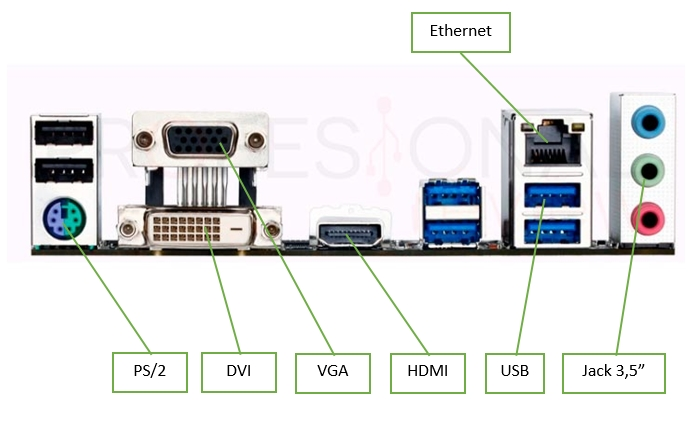
\includegraphics[width=0.8\textwidth]{pcmobo.jpg}
	\caption{Conectores de placa para PC}
\end{figure}

\begin{figure}[H]
	\centering
	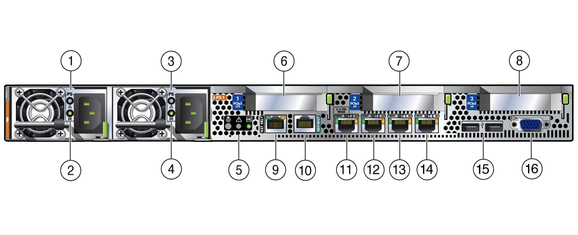
\includegraphics[width=0.8\textwidth]{serverconnectors.jpg}
	\caption{Conectores de placa para servidor}
\end{figure}

\subsection{RJ-45}

\begin{itemize}
	\item Sirve para conectar redes de área local a largas distancias (100m con par trenzado y varios km con fibra óptica).
	\item Los estándares son retrocompatibles y admiten full-dúplex.
	\item Muchos estándares de comunicación se pueden realizar a través de Ethernet:
	\begin{itemize}
		\item iSCSI (\textit{\textbf{I}nternet \textbf{SCSI}}): permite usar SCSI sobre redes TCP/IP.
		\item FCoE (\textit{\textbf{F}ibre \textbf{C}hannel \textbf{o}ver \textbf{Ethernet}}): permite usar tramas Fibre Channel sobre TCP/IP.
	\end{itemize}
\end{itemize}

\begin{figure}[H]
	\centering
	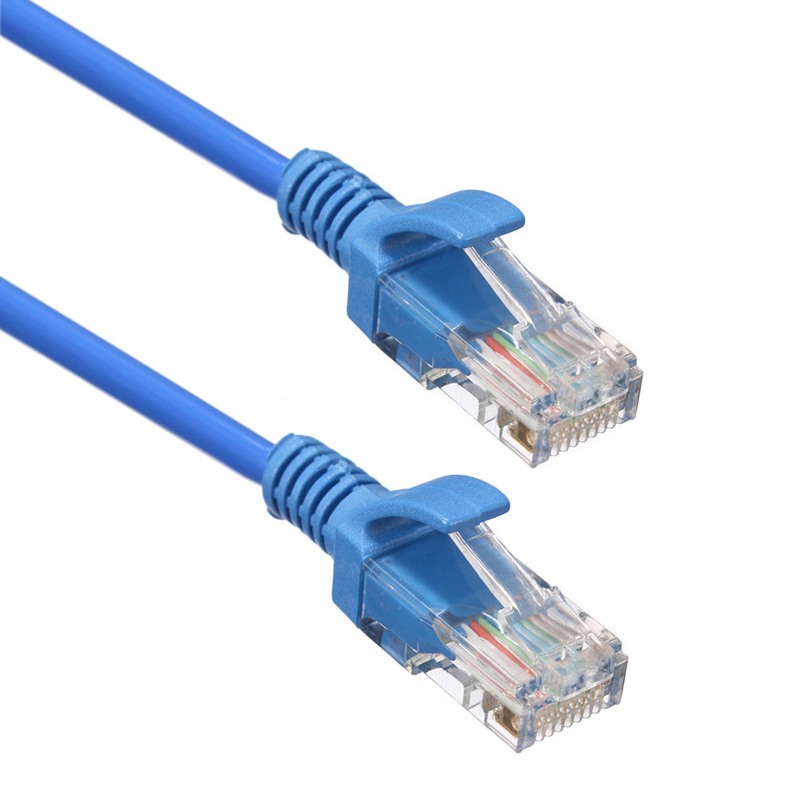
\includegraphics[width=0.3\textwidth]{rj45.jpg}
	\caption{Cable RJ-45}
\end{figure}

\subsection{Universal Serial Bus (USB)}

Actualmente se comercializan dos versiones:
\begin{itemize}
	\item USB 2.0
	\begin{itemize}
		\item Es un puerto de serie de 4 pines (2 de datos, 1 de masa y 1 de alimentación).
		\item Su velocidad máxima es de 480Mb/s.
		\item Soporta hot plug y opera mediante half-dúplex.
	\end{itemize}
	\item USB 3.0
	\begin{itemize}
		\item Se compone de 9 pines: 4 del USB 2.0 (es retrocompatible) y 5 para aportar más velocidad.
		\item Su velocidad máxima es de 4.8Gb/s.
		\item Su sucesor, USB 3.1, soporta hasta 10Gb/s.
	\end{itemize}
\end{itemize}

\begin{figure}[H]
	\centering
	\includegraphics[width=0.3\textwidth]{usb.png}
	\caption{Conectores USB 2.0 y 3.0}
\end{figure}

\subsection{Thunderbolt}

\begin{itemize}
	\item Es un estándar lanzado por Intel.
	\item Combina PCIe y DisplayPort (almacenamiento externo de altas prestaciones y monitor de alta resolución.
	\item Se alcanzan anchos de banda de hasta 40Gb/s en cada dirección y por cada canal.
	\item Utiliza el mismo conector que USB C.
\end{itemize}

\begin{figure}[H]
	\centering
	\includegraphics[width=0.3\textwidth]{thunderbolt.png}
	\caption{Cable Thunderbolt}
\end{figure}

\subsection{Otros conectores internos}

\subsubsection{System panel}

Sirve para conectar los botones de power y reset, luces de encendido y HDD, zumbador, etc. del chasis a la placa base.

\begin{figure}[H]
	\centering
	\includegraphics[width=0.5\textwidth]{syspanel.jpg}
	\caption{Conector del panel del sistema}
\end{figure}

\subsubsection{Puerto de serie}

Sirve para añadir un puerto de serie a la parte trasera de la máquina.


\begin{figure}[H]
	\centering
	\includegraphics[width=0.5\textwidth]{serial.jpg}
	\caption{Conector del puerto de serie}
\end{figure}

\subsubsection{USB interno}

Añade más puertos USB a la máquina. Pueden ser 2.0 o 3.0.

\begin{figure}[H]
	\centering
	\includegraphics[width=0.5\textwidth]{mobousb.jpg}
	\caption{Cable USB 3.0 y conectores USB (2.0 el blanco y 3.0 el azul)}
\end{figure}

\subsubsection{Chassis Intrusion Detector}

Envía una señal cuando se abre la tapa del chasis. Esta señal puede redirigirse a un administrador del sistema. Funciona con el voltaje 5V de standby.

\begin{figure}[H]
	\centering
	\includegraphics[width=0.5\textwidth]{chassisintrusion.jpg}
	\caption{Interruptor para detectar la intrusión en el chasis}
\end{figure}

\subsubsection{IEEE 1394a (Firewire)}

Sirve para conectar dispositivos en serie a gran velocidad. Fue sustituido por USB.

\begin{figure}[H]
	\centering
	\includegraphics[width=0.5\textwidth]{firewire.png}
	\caption{Conector Firewire}
\end{figure}

\subsubsection{CD IN audio}

Servía para el conector de audio de las lectoras de CD PATA. Fue sustituido por conectores de audio en el propio chasis.

\begin{figure}[H]
	\centering
	\includegraphics[width=0.5\textwidth]{cdin.jpg}
	\caption{Conector CD IN}
\end{figure}

\subsection{ROM/Flash BIOS (\textit{\textbf{B}asic \textbf{I}nput \textbf{O}utput \textbf{S}ystem})}

\begin{itemize}
	\item Almacena el código de arranque del computador, que se encarga de identificar los dispositivos instalador, instalar controladores básicos para poder acceder a ellos, realizar el POST (\textit{\textbf{P}ower \textbf{O}n \textbf{S}elf \textbf{T}est}) del sistema e iniciar el SO.
	\item Los parámetros de configuración se almacenan en una memoria RAM alimentada por una pila (que también se usa para el reloj de tiempo real). Algunos de estos parámetros se configuran mediante \textit{jumpers} (conectan dos o más pines) en la placa base, pero la mayoría se gestionan desde el firmware de la BIOS.
\end{itemize}

\begin{figure}[H]
	\centering
	\includegraphics[width=0.5\textwidth]{biosbattery.jpg}
	\caption{Chip BIOS y pila}
\end{figure}

\begin{figure}[H]
	\centering
	\includegraphics[width=0.5\textwidth]{bios.png}
	\caption{Firmware de la BIOS}
\end{figure}

\begin{figure}[H]
	\centering
	\includegraphics[width=0.5\textwidth]{jumper.jpg}
	\caption{\textit{Jumper} para borrar la configuración del firmware de la BIOS}
\end{figure}

\subsection{Chipset}
El chipset es el conjunto de circuitos integrados (chips) de la placa base encargados de controlar las comunicaciones que se realizan. Se divide en dos partes:
\begin{itemize}
	\item \textbf{Puente norte}. Se encarga de las transferencias de mayor velocidad (CPU, GPu, RAM y south bridge).
	\item \textbf{Puente sur}. Se encarga de las transferencias entre el puente norte y el resto de periféricos con menores exigencias de velocidad.
\end{itemize}
\begin{figure}[H]
	\centering
	\includegraphics[width=0.75\textwidth]{chipset.png}
	\caption{Esquema de un chipset}
\end{figure}
En equipos modernos el puente norte se integra en la CPU.
\begin{figure}[H]
	\centering
	\includegraphics[width=0.75\textwidth]{newchipsets.png}
	\caption{Chipsets modernos}
\end{figure}
\subsection{Carcasa (chasis)}
En el mundo de los servidores las carcasas se miden en \emph{Rack Units} (U). Esta medida representa la altura de la carcasa (unos 4.5cm). De esta forma podemos encontrar racks de 42U, 19U, etc.
\begin{figure}[H]
	\centering
	\includegraphics[width=0.5\textwidth]{rackunits.png}
	\caption{Rack Units}
\end{figure}
\subsection{CPD: Centros de Procesamiento de Datos}
Son ubicaciones en las que se concentran los recursos informáticos necesarios para el procesamiento de grandes volúmenes de datos.
\begin{itemize}
	\item Los servidores, switches, etc. se almacenan en armarios o racks.
	\item El cableado se distribuye en bandejas, falsos suelos o techos, etc.
	\item La alimentación es redundante.
	\item La ventilación es muy importante.
\end{itemize}

\begin{figure}[H]
	\centering
	\includegraphics[width=0.5\textwidth]{cpd.jpg}
	\caption{Centro de Procesamiento de Datos}
\end{figure}
\newpage
\section{Tema 3. Monitorización de servicios y programas}

\subsection{Concepto de monitor de actividad}
\begin{itemize}
	\item \textbf{Carga} (workload). Es el conjunto de tareas que ha de realizar un sistema, todo aquello que demande recursos.
	\item \textbf{Actividad} de un sistema. Es el conjunto de operaciones que se realizan en el sistema como consecuencia de la carga que soporta.
	\item Un sistema informático no es ''bueno'' ni ''malo'', sino que se adapta mejor o peor a un determinado tipo de carga.
	\item La actividad del sistema puede variar debido a los procesadores, la memoria, los discos, la red, etc.
\end{itemize}

Un \textbf{monitor de actividad} es una herramienta diseñada para medir la actividad de un sistema informático y facilitar su análisis. Se encarga de medir alguna variable que refleje la actividad del sistema, procesar y almacenar los datos recopilados y mostrarlos.

Su utilidad depende de la persona que lo utilice:
\begin{itemize}
	\item Administrador/Ingeniero
	\begin{itemize}
		\item Conocer el uso de recursos para detectar cuellos de botella.
		\item Predecir cargas futuras.
		\item Tarificar a los clientes (cloud).
		\item Poder deducir qué pasaría si...
	\end{itemize}
	\item Programador: conocer las partes críticas de una aplicación de cara a la optimización.
	\item Sistema Operativo: adaptarse dinámicamente a la carga.
\end{itemize}

Hay varios tipos de monitores dependiendo del momento en el que se realicen las medidas:
\begin{itemize}
	\item \textbf{Monitor por eventos}. Se mide cuando ocurre un evento (inicio/fin de programa, fallo de caché, etc.). Proporcionan información exacta.
	\item \textbf{Monitor por muestreo}. Toma medidas cada x tiempo. La información que proporciona es estadística.
\end{itemize}

Si atendemos a la forma en la que se mide, podemos distinguir entre:
\begin{itemize}
	\item Software: programas instalados en el sistema.
	\item Hardware: dispositivos físicos de medida (la sobrecarga es menor).
	\item Híbridos: mezcla de los dos anteriores.
\end{itemize}

Por último, podemos clasificar los monitores según si existe interacción con el usuario:

\begin{itemize}
	\item No existe: la consulta de los resultados se realiza mediante otra herramienta independiente al proceso de monitorización (monitores por lotes o en segundo plano).
	\item Sí existe. Durante el proceso de monitorización se pueden consultar los valores y/o interactuar con ellos realizando representaciones gráficas, modificando parámetros del monitor, etc. (monitores en primer plano o interactivos).
\end{itemize}

Los atributos que caracterizan a un monitor son:

\begin{itemize}
	\item \textbf{Exactitud} de la medida (\textit{accuracy, offset}). ¿Cuánto se aleja el valor medido del valor real?
	\item \textbf{Precisión}. ¿Cuál es la dispersión de las medidas?
	\item \textbf{Resolución} del sensor. ¿Cuánto tiene que cambiar el valor a medir para detectar un cambio?
	\item \textbf{Tasa máxima de entrada} (\textit{max input rate}). ¿Cuál es la frecuencia máxima que el monitor puede observar? (monitores por eventos).
	\item \textbf{Período de muestreo} (\textit{sampling time}). ¿Cada cuánto tiempo tomamos la medida? (monitores por muestreo).
	\item \textbf{Anchura de entrada} (\textit{input width}). ¿Cuánta información se almacena por cada medida tomada?
	\item \textbf{Sobrecarga} (\textit{overhead}). ¿Qué recursos le ''roba'' en monitor al sistema?
	\[
		Sobrecarga_{recurso}(\%) = \frac{Uso\ del\ recurso\ por\ parte\ del\ monitor}{Capacidad\ total\ del\ recurso} \times 100
	\]
	Ejemplo: calcular la sobrecarga de CPU de un monitor software por muestreo. El monitor se activa cada 5 s y cada activación usa la CPU durante 6 ms.
	\[
		Sobrecarga_{CPU}(\%) = \frac{6 \times 10^{-3} s}{5 s} \times 100 = 0.12\%
	\]
\end{itemize}

\subsection{Monitorización a nivel de sistema}

Unix dispone de un directorio (\textit{/proc}) que es muy importante para la monitorización:
\begin{itemize}
	\item Es una carpeta en RAM que facilita el acceso del usuario a las estructuras de datos del SO.
	\item Podemos acceder a multitud de información sobre el SO:
	\begin{itemize}
		\item Global: \textit{loadavg, uptime, meminfo, mdinfo}, etc.
		\item Sobre cada proceso \textit{/proc/<pid>}.
		\item Parámetros del kernel (\textit{/proc/sys}).
	\end{itemize}
\end{itemize}
La mayoría de monitores utilizan este directorio como fuente de información.

\subsubsection{Uptime}
Indica el tiempo que el sistema lleva en marcha y la carga media que soporta.
\begin{lstlisting}
	$> uptime
<hora actual> up <tiempo en marcha>,  <numero de usuarios>,  load average: <ultimo minuto>, <ultimos 5 minutos>, <ultimos 15 minutos>
\end{lstlisting}
Por ejemplo:
\begin{lstlisting}
	$> uptime
	17:53:58 up 11 min,  1 user,  load average: 1,59, 1,15, 0,67
\end{lstlisting}

\subsubsection{Carga del sistema Unix}

En Unix los procesos pueden encontrarse en los siguientes estados:
\begin{itemize}
	\item \textbf{En ejecución} (\textit{running}) o en la cola de ejecución (\textit{runnable}).
	\item \textbf{Bloqueado} (\textit{I/O blocked}), está esperando una operación de E/S.
	\item \textbf{Durmiendo} (\textit{sleeping}), se está esperando un evento del usuario (por ejemplo, una pulsación de tecla)
\end{itemize}
La cola de procesos del núcleo (\textit{run queue}) está formada por aquellos que pueden ejecutarse (\textit{runnable + running}).\\

La \textbf{carga del sistema} es el número de procesoss que hay en modo \textit{running, runnable} o \textit{I/O blocked} (en ejecución, en cola de ejecución o bloqueados por E/S).

\subsubsection{Ps (\textit{process status})}
Esta herramienta nos proporciona información sobre el estado actual de los procesos del sistema.
\begin{figure}[H]
	\centering
	\includegraphics[width=0.75\textwidth]{psaur.png}
	\caption{ps aur}
\end{figure}

\begin{itemize}
	\item \textbf{\textit{USER}}. Usuario que lanzó el proceso.
	\item \textbf{\textit{\% CPU, \% MEM}}. Porcentaje de CPU y memoria usada.
	\item \textbf{\textit{RSS}} (\textit{Resident Set Size}). Memoria ocupada por el proceso.
	\item \textbf{\textit{STAT}}. Estado en el que se encuentra el proceso:
	\begin{itemize}
		\item \textbf{R (\textit{running or runnable}), D (\textit{I/O Blocked})}
		\item \textbf{S (\textit{interruptible sleep}), T (\textit{stopped})}
		\item \textbf{Z (\textit{zombie})}. Terminated but not dead.
	\end{itemize}
\end{itemize}

\subsubsection{Top}
Este comando muestra estadísticas como la carga media, procesos, consumo de memoria, etc. cada T segundos. Normalmente se ejecuta en modo interactivo (se elige el valor de T, las columnas mostradas, el orden de las filas, etc.)

\begin{figure}[H]
	\centering
	\includegraphics[width=0.75\textwidth]{top.png}
	\caption{top}
\end{figure}

\subsubsection{vmstat (\textit{Virtual Memory Stadistics})}
Proporciona información sobre paginación, swap, interrupciones, CPU, etc.\\
Debemos despreciar la primera línea, ya que aporta información desde el inicio del sistema.

\begin{figure}[H]
	\centering
	\includegraphics[width=0.75\textwidth]{vmstat.png}
	\caption{vmstat}
\end{figure}

\begin{itemize}
	\item Procesos: \textbf{r} (\textit{runnable}), \textbf{b} (\textit{I/O blocked}).
	\item Bloques por segundos transmitidos: \textbf{bi} (\textit{blocks in}), \textbf{bo} (\textit{blocks out}).
	\item KB/s entre memoria y disco: \textbf{si} (\textit{swapped in}), \textbf{so} (\textit{swapped out}).
	\item \textbf{in} (\textit{interrupts per second}), \textbf{cs} (\textit{context switched per second}).
\end{itemize}

Se le pueden especificar otros argumentos para que proporcione información sobre acceso a discos (en concreto la partición swap) y otras estadísticas.

\subsubsection{sar (\textit{System Activity Recorder})}
Es una herramienta del paquete \textit{systat}. Proporciona información general sobre todo el sistema a partir de la obtenida del directorio \textit{/proc}. Está formado por dos componentes:
\begin{itemize}
	\item sadc (\textit{system-accounting data collector}). Recoge los datos y construye un registro binario.
	\item sar: lee los datos binarios y los traduce a textoi plano.
\end{itemize}

\begin{figure}[H]
	\centering
	\includegraphics[width=0.75\textwidth]{sar.png}
	\caption{sar}
\end{figure}

\subsubsection{Otras herramientas de \textit{systat}}
\begin{itemize}
	\item \textbf{mpstat}. Muestra estadísticas concretas por cada núcleo.
	\item \textbf{iostat}. Muestra estadísticas de los dispositivos de E/S y particiones de disco.
\end{itemize}


\subsection{Monitorización a nivel de aplicación (profiling)}

El objetivo de un \textit{profiler} es monitorizar la actividad generada por una aplicación para obtener información con la que optimizar su código. La información que puede proporcionar un \textit{profiler} puede ser la siguiente:
\begin{itemize}
	\item ¿Cuánto tiempo tarda en ejecutarse el programa? ¿Qué parte de ese tiempo es del usuario, del sistema? ¿Cuánto se invierte en operaciones de E/S?
	\item ¿En qué parte del código se pasa la mayor parte del tiempo (\textit{hot spots})?
	\item ¿Cuántas veces se ejecuta una línea?
\end{itemize}
\subsubsection{time}
El programa \textit{/usr/bin/time} mide el tiempo de ejecución de un programa y muestra algunas estadísticas:
\begin{itemize}
	\item \textit{real}: tiempo total usado por el sistema.
	\item \textit{user}: tiempo de CPU ejecutando en modo usuario.
	\item \textit{sys}: tiempo de CPU ejecutando código del sistema.
	\item Cambios de contexto voluntarios (al tener que esperar a una operación de E/S se cede la CPU a otro proceso).
	\item Cambios de contexto involuntarios: se acaba la rodaja de tiempo.
	\item \textit{Major page faults}: requieren acceder a disco.
\end{itemize}
No debemos confundir \textit{/usr/bin/time} con \textit{time}, que es una versión ligera que nos da mucha menos información (sólo \textit{real}, \textit{user} y \textit{sys}).

\subsubsection{gprof}
Da información sobre el tiempo de CPU y número de veces que se ejecuta cada función de un proceso o hilo en un sistema Unix. Se utiliza de la siguiente forma:
\begin{enumerate}
	\item Compilamos el programa con los flags de profiling y depuración:
	\begin{lstlisting}
		$> gcc prog.c -o prog -pg -g
	\end{lstlisting}
	\item Ejecutamos el programa:
	\begin{lstlisting}
		$> ./prog
	\end{lstlisting}
	\item La información se almacena en el fichero \textit{gmon.out}.
	\item Visualizamos la información con
	\begin{lstlisting}
		$> gprof prog
	\end{lstlisting}
\end{enumerate}

\subsubsection{gcov}

Aporta información sobre el número de veces que se ejecuta cada línea del programa. Se usa de la siguiente forma:

\begin{enumerate}
	\item Compilamos con los siguientes flags:
	\begin{lstlisting}
		$> gcc prog.c -o prog -fprofile-arcs -ftest-coverage
	\end{lstlisting}
	\item Ejecutamos el programa:
	\begin{lstlisting}
		$> ./prog
	\end{lstlisting}
	\item La información se almacena en varios ficheros.
	\item Visualizamos la información con
	\begin{lstlisting}
		$> gcov prog.c
	\end{lstlisting}
\end{enumerate}

\subsubsection{Perf}

\textit{Perf} es un conjunto de herramientas para analizar el rendimiento en Linux. Permiten analizar el rendimiento de un hilo. un proceso y sus hijos, todos los procesos que se ejecutan en una CPU o todos los que se ejecutan en el sistema.

\subsubsection{Valgrind}

Es un conjunto de herramientas para el análisis y la mejora del código. Puede analizar cualquier binario ya compilado (no requiere flags específicos). Básicamente crea una máquina virtual que emula la ejecución del programa en un entorno aislado.

\subsubsection{V-Tune (Intel) y CodeXL (AMD)}

Ofrecen información muy similar a la de Perf. Están disponibles tanto para Windows como para Linux. Se pueden usar también como depuradores.
\newpage
\section{Tema 4: Análisis comparativo del rendimiento}

\subsection{Índices clásicos de rendimiento}

Un buen índice de rendimiento para un sistema informático debe cumplir las siguientes características:
\begin{itemize}
	\item Representatividad y fiabilidad. Si un sistema presenta un índice de rendimiento mayor que otro es porque siempre el rendimiento del primero es mejor.
	\item Repetibilidad. Siempre que se mida el índice en las mismas condiciones el valor deberá ser el mismo.
	\item Consistencia y facilidad de medición. El índice debe poder medirse en cualquier sistema informático y la medida debe ser fácil de tomar.
	\item Linealidad: si el índice de rendimiento aumenta, el rendimiento del sistema también debe aumentar en la misma proporción.
\end{itemize}

\subsubsection{Tiempo de ejecución, frecuencia de reloj y CPI}
$
T_{ejec}=NI \times CPI \times T_{reloj}=\frac{NI \times CPI}{f_{reloj}}
$
No son buenos índices de rendimiento ya que se pueden encontrar sistemas con peores frecuencias o CPI pero con mejores prestaciones. El tiempo de ejecución tampoco es un buen índice, ya que:
\begin{itemize}
	\item Consistencia: el programa debería estar descrito en un lenguaje de alto nivel.
	\item Repetibilidad: el programa debería ejecutarse en un entorno muy controlado.
	\item Representatividad y fiabilidad: depende del programa que se ejecute.
\end{itemize}

\subsubsection{MIPS}
$
MIPS=\frac{NI}{T_{ejec} \times 10^6}=\frac{f_{reloj}}{CPI \times 10^6}
$
Desventajas: depende del número de instrucciones y los MIPS pueden variar entre programas en la misma máquina.

\subsubsection{MFLOPS}

Está basado en operaciones, no en instrucciones.
$
MFLOPS=\frac{Operaciones_{float}}{T_{ejec} \times 10^6}
$
Inconvenientes:
\begin{itemize}
	\item No todas las operaciones en coma flotante tienen la misma complejidad, por lo que debemos ponderar cada operación multiplicándola por un peso.
	\item El formato de los números en coma flotante puede variar de una arquitectura a otra, por lo que la precisión puede variar también.
\end{itemize}
Conclusión final: no existe un índice de rendimiento perfecto. Nos contentaremos con el tiempo de ejecución ($t_{ejec}$) de un programa o conjunto de programas, por lo que el resultado dependerá de la carga del PC.

\subsection{Benchmarking}

Un modelo de carga es una aproximación de la carga que recibe un sistema informático. El modelo de carga debe ser lo más representativo y simple posible. Existen dos estrategias para obtener modelos de carga:
\begin{itemize}
	\item Ajustar un modelo paramétrico personalizado (caracterización de la carga).
	\item Usar programas de prueba que utilicen un modelo genérico de carga lo más similar posible al que se quiere reproducir (referenciación, benchmarking).
\end{itemize}

\subsubsection{Tipos de benchmarks}

Los benchmarks se pueden clasificar:
\begin{itemize}
	\item Según la estrategia de medida
	\begin{itemize}
		\item Programas que miden el tiempo necesario para ejecutar una cantidad prefijada de tareas (la mayoría).
		\item Programas que miden la cantidad de tareas ejecutadas en un tiempo prefijado.
		\item Programas que permiten variar tanto la cantidad de tareas como el tiempo para adaptarlos a cada sistema.
	\end{itemize}
	\item Según la generalidad del test:
		\begin{itemize}
			\item Microbenchmarks o benchmarks para componentes. Estresan componentes concretos.
			\item Macrobenchmarks o benchmarks de sistema completo o aplicación real. Intentan imitar situaciones reales.
		\end{itemize}
\end{itemize}

\subsection{Análisis de los resultados de un test de rendimiento}

El rendimiento es una variable multidimensional, por lo que debería expresarse mediante varios índices. Sin embargo, las comparaciones son más sencillas si se usa un único índice de rendimiento.\\

Para unificar los índices podemos seleccionar el mejor o bien tenerlos todos en cuenta utilizando algún tipo de media.

\subsubsection{Media aritmética}

\begin{equation*}
	\overline{t}=\frac{1}{n}\sum{t_k}
\end{equation*}

Si las medidas no tienen igual importancia, podemos asociar a cada medida $t_k$ un peso $w_k$, obteniendo la \textbf{media aritmética ponderada}:
\begin{equation*}
	\overline{t_w}=\frac{1}{n}\sum{w_k \times t_k}
\end{equation*}

El peso puede ser inversamente proporcional al tiempo de ejecución de una máquina de referencia:
\begin{equation*}
	w_k=\frac{C}{t_k^{ref}}
\end{equation*}
\begin{equation*}
	C=\frac{1}{\sum{\frac{1}{t_k^{ref}}}}
\end{equation*}

\subsubsection{Media geométrica}

\begin{equation*}
	\overline{S_g}=\sqrt[n]{\prod{S_k}}=(\prod{S_k})^{\frac{1}{n}}
\end{equation*}

Propiedad: cuando las medidas son ganancias en velocidad (speedups) con respecto a una máquina de referencia, este índice mantiene el mismo orden en las comparaciones independientemente de la máquina de referencia elegida. Esta propiedad se usa en los benchmarks SPEC y SYSMARK.

\begin{equation*}
	SPEC(M)=\sqrt[n]{\frac{t_{1}^{ref}}{t_{1}^{M}} \times \frac{t_{2}^{ref}}{t_{2}^{M}} \times ... \times \frac{t_{n}^{ref}}{t_{n}^{M}}} = \frac{\sqrt[n]{t_{1}^{ref} \times t_{2}^{ref} \times ... \times t_{n}^{ref}}}{\sqrt[n]{t_{1}^{M} \times t_{2}^{M} \times ... \times t_{n}^{M}}}
\end{equation*}

En los benchmarks elegimos la media geométrica de speedups como índice de rendimiento para premiar las mejoras sustanciales y no castigar tanto los empeoramientos. Además, no depende de la máquina de referencia.
\newpage
\subsection{Comparación de prestaciones en presencia de aleatoriedad}

\subsubsection{Repaso de estadística: distribución normal}

La distribución normal está caracterizada por la media $\mu$ y la varianza $\sigma^2$. La función de probabilidad viene dada por:
\begin{equation*}
	Prob(x) = \frac{1}{\sqrt{2\pi\sigma^2}}\times e^{\frac{(x-\mu)^2}{2\sigma^2}}
\end{equation*}
La probabilidad de obtener un elemento en el rango $[\mu - 2\sigma, \mu + 2\sigma]$ es del 95\%.\\
\textbf{Teorema del límite central}: la suma de un conjunto grande de muestras aleatorias de cualquier distribución e independientes entre sí pertenece a una distribución normal.
\begin{figure}[H]
	\centering
	\includegraphics[width=0.5\textwidth]{normal.png}
	\caption{Distribución normal con $\mu=0$ y $\sigma=1$}
\end{figure}

\subsubsection{Repaso de estadística: distribución t de Student}

Si disponemos de $n$ muestras $d_i$ pertenecientes a una Normal con media $d_{real}$ y calculamos $t_{exp}$ (al que llamaremos estadístico):
\begin{equation*}
	t_{exp}=\frac{\overline{d}-\overline{d_{real}}}{\frac{s}{\sqrt{n}}}
\end{equation*}
siendo $\overline{d}$ la media muestral y $s$ la desviación típica muestral:
\begin{equation*}
	\overline{d}=\frac{\sum{d_i}}{n}
\end{equation*}
\begin{equation*}
	s=\sqrt{\frac{\sum{(d_i-\overline{d})^2}}{n-1}}
\end{equation*}
y repetimos el experimento muchas veces, veremos que esos $t_{exp}$ se distribuyen según la distribución t de Student con $n-1$ grados de libertad.\\
\textbf{Para $n>30$, la distribución normal y la t de Student coinciden.}

\begin{itemize}
	\item \textbf{Nivel o grado de significatividad ($\alpha$)}. Es el nivel de confianza que estableceremos para realizar nuestro análisis.
	\item \textbf{P-value}. Probabilidad de obtener un valor de $|t|$ en una distribución t de Student con n grados de libertad. Si $\alpha>p-value$ rechazaremos $H_0$.
	\item \textbf{Intervalos de confianza para $t{exp}$}. Para aceptar nuestra hipótesis nula, el valor de $t_{exp}$ debe situarse en el intervalo $[-t_{\frac{\alpha}{2},n-1}, t_{\frac{\alpha}{2},n-1}]$. Este intervalo se denomina intervalo de confianza para un nivel de significatividad $\alpha$.
	\item \textbf{Intervalos de confianza para $\overline{d_{real}}$}. Aceptaremos la hipótesis nula si $\overline{d_{real}}$ pertenece al intervalo $[\overline{d}-\frac{s}{\sqrt{n}} \times t_{\frac{\alpha}{2},n-1}, [\overline{d}+\frac{s}{\sqrt{n}} \times t_{\frac{\alpha}{2},n-1}]$.
\end{itemize}

\begin{figure}[H]
	\centering
	\includegraphics[width=0.5\textwidth]{intconf.png}
	\caption{Intervalo de confianza (en blanco)}
\end{figure}

\subsubsection{Ejemplo: test de rendimiento entre A y B}
Ejecutamos seis programas en dos máquinas (A y B) y obtenemos los siguientes tiempos (en segundos):
\begin{figure}[H]
	\centering
	\begin{tabular}{|c|c|c|c|}
		\hline
		Programa & $t_A$ & $t_B$ & $d_i=t_{A_i}-t_{B_i}$\\
		\hline
		P1 & 142 & 100 & 42 \\
		\hline
		P2 & 139 & 92 & 47 \\
		\hline
		P3 & 152 & 128 & 24\\
		\hline
		P4 & 112 & 82 & 30\\
		\hline
		P5 & 156 & 148 & 8\\
		\hline
		P6 & 166 & 171 & -5\\
		\hline
		Suma & 867 & 721 & -\\
		\hline
	\end{tabular}
	\caption{Tiempos de ejecución}
\end{figure}
Calculamos la media muestral y la desviación típica muestral:
\begin{equation*}
	\overline{d}=\frac{\sum{d_i}}{n}=\frac{42+47+24+30+8+(-5)}{6}=\frac{146}{6}=24.3 seg
\end{equation*}
\begin{gather*}
		s=\sqrt{\frac{\sum{(d_i-\overline{d})^2}
		}{n-1}}=\\
		=\sqrt{\frac{(42-24.3)^2+(47-24.3)^2+(24-24.3)^2+(30-24.3)^2+(8-24.3)^2+((-5)-24.3)^2}{6-1}} =\\ = \sqrt{\frac{1985.34}{5}}=19.9 seg
\end{gather*}

Partimos de la hipótesis nula $H_0$: las máquinas tienen rendimientos equivalentes. Esto implica que las diferencias se deben a una suma de factores aleatorios independientes. Por tanto, $d_i$ serán muestras de una normal con media cero $\overline{d_{real}}=0$. Por tanto:
\begin{equation*}
	t_{exp}=\frac{\overline{d}}{\frac{s}{\sqrt{n}}}=\frac{24.3 seg}{\frac{19.9 seg}{\sqrt{6}}}=2.99
\end{equation*}
pertenecerá a una distribución t de Student con $n-1=6-1=5$ grados de libertad.\\
Podemos hallar la solución al problema de dos formas: intervalos de confianza o p-value.
\paragraph{P-value}
El P-value (probabilidad de obtener un $|t|$ mayor o igual a $2.99$ en una distribución t de Student con 5 grados de libertad) es de $0.03$. Si tomamos un nivel de confianza del 95\%, $(1-\alpha) \times 100 = 95\% \implies \alpha=0.05$. Como $\alpha=0.05 > 0.03 = p-value$, rechazamos $H_0$. Es decir, las máquinas tienen rendimientos estadísticamente diferentes. En este caso, B es $\frac{867}{721}=1.2$ veces más rápida que A para ejecutar el conjunto de programas. Si hubiéramos aceptado $H_0$, no podríamos descartar que las máquinas tuvieran rendimientos equivalentes.
\paragraph{Intervalos de confianza}

\subparagraph{Para $t_{exp}$}

El valor $t_{\frac{\alpha}{2},n-1}=t_{\frac{0.05}{2},5}=t_{0.025,5}$ es $2.57$. Por tanto, el intervalo sería $[-2.57,2.57]$. Como $t_{exp}=2.99 \not \in [-2.57,2.57]$, rechazamos $H_0$.

\subparagraph{Para $\overline{d_{real}}$}

El intervalo sería $[\overline{d}-\frac{s}{\sqrt{n}} \times t_{\frac{\alpha}{2},n-1}, \overline{d}+\frac{s}{\sqrt{n}} \times t_{\frac{\alpha}{2},n-1}]= [24.3 - 20.9, 24.3 + 20.9] = [3'4, 42'2]$. Como $0 \not \in [3.4, 42.2]$, rechazamos $H_0$.

\subsubsection{Ejemplo 2}
Calcular un intervalo de confianza del $95\%$ para el tiempo medio de escritura que se ha medido en $n=8$ experimentos. Dato: $t_{0.025,7}=2.36$.
\begin{figure}[H]
	\centering
	\begin{tabular}{|c|c|}
		\hline
		Experimento & tiempo (ms)\\
		\hline
		1 & 835 \\
		\hline
		2 & 798 \\
		\hline
		3 & 823\\
		\hline
		4 & 803\\
		\hline
		5 & 834\\
		\hline
		6 & 825\\
		\hline
		7 & 813\\
		\hline
		8 & 829\\
		\hline
	\end{tabular}
	\caption{Tiempos de escritura}
\end{figure}

El intervalo para la media es de la forma:
\begin{equation*}
	[\overline{d}-\frac{s}{\sqrt{n}} \times t_{\frac{\alpha}{2},n-1}, \overline{d}+\frac{s}{\sqrt{n}} \times t_{\frac{\alpha}{2},n-1}]
\end{equation*}

Por tanto, calculamos los parámetros necesarios:
\begin{itemize}
	\item $\overline{d}=\frac{\sum{d_i}}{n}=820ms$
	\item $s=\sqrt{\frac{\sum{(d_i-\overline{d})^2}}{n-1}}=14ms$
	\item $(1-\alpha) \times 100 = 95 \implies \alpha=0.05$
\end{itemize}

Por tanto, el intervalo será $	[820-\frac{14}{\sqrt{8}} \times 2.36, 820+\frac{14}{\sqrt{8}} \times 2.36] = [808,832]ms$.
\newpage
\section{Tema 5: Análisis operacional en servidores}

\subsection{Redes de colas de espera}

Un modelo de sistema informático es una abstracción de un sistema informático real. Consta de:
\begin{itemize}
	\item Dispositivos (recursos): procesador, memoria, discos, etc.
	\item Trabajos: procesos, peticiones, accesos, etc.
\end{itemize}

Normalmente un dispositivo o recurso sólo se puede usar por un trabajo a la vez. El resto de trabajos tendrán que esperar.\\

Los \textbf{modelos basados en redes de colas} ofrecen una aproximación estadística del tiempo que necesita el sistema para procesar cada trabajo (tiempo de respuesta).

\begin{figure}[H]
	\centering
	\includegraphics[width=0.5\textwidth]{redcolas.png}
	\caption{Red de colas}
\end{figure}

Una \textbf{red de colas} es un conjunto de estaciones conectadas entre sí. Una \textbf{estación de servicio} es una abstracción compuesta por un dispoisitivo (recurso físico) que presta un servicio y una cola de espera para los trabajos (clientes).

\begin{figure}[H]
	\centering
	\includegraphics[width=0.5\textwidth]{estserv.png}
	\caption{Estación de servicio}
\end{figure}

\subsubsection{Modelo de servidor central}

Es el modelo de redes de colas más utilizado para expresar el comportamiento básico de los programas en un servidor de cara a extraer información sobre el rendimiento.
\begin{itemize}
	\item Un trabajo que ''llega'' al servidor comienza utilizando el procesador.
	\item Después de abandonar el procesador, el trabajo puede:
		\begin{itemize}
			\item Terminar (salir del servidor).
			\item Realizar un acceso a E/S (discos, red...).
		\end{itemize}
		\item Tras una operación de E/S, el trabajo vuelve a visitar al procesador.
\end{itemize}

\begin{figure}[H]
	\centering
	\includegraphics[width=0.75\textwidth]{modelocentral.png}
	\caption{Modelo de servidor central}
\end{figure}

\subsubsection{Variables que caracterizan a un trabajo en un estación de servicio}

\begin{itemize}
	\item \textbf{W}, \textit{waiting time}, tiempo de espera en cola. Tiempo desde que el trabajo solicita usar el recurso hasta que comienza a usarlo.
	\item \textbf{S}, \textit{service time}, tiempo de servicio. Tiempo desde que el trabajo accede al recurso hasta que lo libera.
	\item \textbf{R}, \textit{response time}, tiempo de respuesta. Suma de los tiempos anteriores (desde que el trabajo solicita usar el recurso hasta que lo libera). $R = W + S$
\end{itemize}

\begin{figure}[H]
	\centering
	\includegraphics[width=0.3\textwidth]{variablesestserv.png}
	\caption{Variables de un trabajo en una estación de servicio}
\end{figure}

\subsubsection{Ejercicio}

Suponga que una estación de servicio tiene un tiempo de servicio constante $S=1s$. Suponga que los trabajos llegan de la siguiente forma:
\begin{itemize}
	\item Durante los 5 primeros segundos no llega ninguno.
	\item En $t=5s$ llegan $J_1$, $J_2$ y $J_3$ en ese orden.
\end{itemize}
Calcule los tiempos de espera en la cola y los tiempos de respuesta que experimenta cada trabajo. Calcule los valores medios de $W$ y $R$.\\

El esquema sería el siguiente:

\begin{figure}[H]
	\centering
	\includegraphics[width=0.75\textwidth]{t5ej.png}
	\caption{Esquema de la estación de servicio}
\end{figure}

Calculemos los valores:
\begin{itemize}
	\item $W(J_1)$. $J_1$ comienza a ejecutarse nada más llegar, por lo que $W(J_1)=0$.
	\item $R(J_1)$= $W(J_1) + S(J_1)=1s$.
	\item $W(J_2)$. $J_2$ comienza a ejecutarse en $t=6s$, por lo que $W(J_2)=1$.
	\item $R(J_2)$= $W(J_2) + S(J_2)=2s$.
	\item $W(J_3)$. $J_3$ comienza a ejecutarse en $t=7s$, por lo que $W(J_3)=2$.
	\item $R(J_3)$= $W(J_3) + S(J_3)=3s$.
	\item $\overline{W}=1s$.
	\item $\overline{R}=2s$.
\end{itemize}

\subsubsection{Estaciones con más de un servidor}

Son las que permiten atender más de un trabajo en paralelo:

\begin{figure}[H]
	\centering
	\includegraphics[width=0.75\textwidth]{estpar.png}
	\caption{Tipos de estación con más de un servidor}
\end{figure}

\subsubsection{Tiempo de reflexión (Z, think time)}

Es un parámetro que representa el tiempo que requiere el usuario antes de volver a lanzar una petición al servidor tras la respuesta de éste. Se suele modelar mediante una estación de servicio de tipo retardo con $S=Z$.

\begin{figure}[H]
	\centering
	\includegraphics[width=0.75\textwidth]{thinktime.png}
	\caption{Tiempo de reflexión}
\end{figure}

\subsubsection{Redes de colas cerradas}

Presentan un número constante de trabajos que van recirculando por la red ($N_T$). Hay dos tipos:
\begin{itemize}
	\item Por lotes (\textit{batch}). No hay interacción con el usuario, los trabajos van pasando uno a uno.
	\item Interactivas. Se espera a que el usuario vuelva a introducir los trabajos en el servidor.
\end{itemize}

\begin{figure}[H]
	\centering
	\includegraphics[width=0.75\textwidth]{cerradas.png}
	\caption{Tipos de redes de colas cerradas}
\end{figure}

\subsubsection{Redes de colas abiertas}

Los trabajos llegan a la red a través de una fuente externa no controlada. Tras ser procesados, salen de ella por uno o más sumideros. No hay retroalimentación entre sumidero y fuente.

\begin{figure}[H]
	\centering
	\includegraphics[width=0.75\textwidth]{abiertas.png}
	\caption{Red de colas abierta}
\end{figure}

\subsubsection{Redes de colas mixtas}

Son una mezcla de las dos anteriores:

\begin{figure}[H]
	\centering
	\includegraphics[width=0.75\textwidth]{mixtas.png}
	\caption{Red de colas abierta}
\end{figure}


\subsection{Variables y leyes operacionales}

\subsubsection{Análisis operacional}

El análisis operacional es una técnica de análisis de colas que se basa en los valores medios de las variables operacionales (magnitudes medibles) del sistema informático. Nos permite calcular límites optimistas de las prestaciones del servidor.\\

Las \textbf{leyes operacionales} son las relaciones que hay entre las variables operacionales.

\begin{itemize}
	\item Un servidor contiene $K$ estaciones de servicio (recursos o dispositivos),
	\item A todo el servidor en su globalidad lo denominamos dispositivo ''cero''
\end{itemize}

\subsubsection{Variables operacionales básicas}

\begin{itemize}
	\item $\pmb{T}$. Duración del periodo de medida. Es una variable global.
	\item $\pmb{A_i}$. Número de trabajos solicitados a la estación $i$ (llegadas, \textit{arrivals}).
	\item $\pmb{B_i}$. Tiempo que la estación $i$ está ocupada (\textit{busy time}).
	\item $\pmb{C_i}$. Número de trabajos completados por la estación (\textit{completions}).
\end{itemize}

\begin{figure}[H]
	\centering
	\includegraphics[width=0.75\textwidth]{varbasicas.png}
	\caption{Variables operacionales básicas}
\end{figure}

\subsubsection{Variables operacionales deducidas}

Estas variables se estiman a partir de las básicas
\begin{itemize}
	\item $\pmb{\lambda_i}$. Tasa media de llegada (\textit{arrival rate}) (trabajos/segundo).
	\item $\pmb{X_i}$. Productividad media (\textit{throughput}) (trabajos/segundo).
	\item $\pmb{S_i}$. Tiempo medio de servicio (\textit{service time}) (segundos).
	\item $\pmb{W_i}$. Tiempo medio de espera en cola (\textit{waiting time}) (segundos).
	\item $\pmb{R_i}$. Tiempo medio de respuesta (\textit{response time}) (segundos).
	\item $\pmb{U_i}$. Utilización media (\textit{utilization}) (sin unidad).
\end{itemize}

\begin{figure}[H]
	\centering
	\includegraphics[width=0.75\textwidth]{vardeduc.png}
	\caption{Variables operacionales deducidas}
\end{figure}

\begin{itemize}
	\item $\pmb{N_i}$. Número medio de trabajos en la estación de servicio ($cola + recurso$).
	\item $\pmb{Q_i}$. Número medio de trabajos en cola de espera (\textit{jobs in queue}). Se calcula sumando el producto del tiempo por el número de trabajos esperando en cada intervalo y dividiéndolo entre $T$:
	\begin{equation*}
			Q_i= \frac{\splitfrac{tiempo(t \in [0,1)) \times trabajos_{espera}(t \in [0,1) +}{ ... + tiempo(t \in [T-1,T)) \times trabajos_{espera}(t \in [T-1,T)}}{T}
	\end{equation*}

	\item $\pmb{U_i}$. Número medio de trabajos siendo servidos por el dispositivo. $U_i=N_i - Q_i$. Coincide numéricamente con la utilización media.
\end{itemize}

\begin{figure}[H]
	\centering
	\includegraphics[width=0.75\textwidth]{vardeduc2.png}
	\caption{Variables operacionales deducidas (2)}
\end{figure}

\subsubsection{Ejercicio}

Suponga que una estación de servicio tiene un tiempo de servicio constante $S=1s$. Suponga que los trabajos llegan de la siguiente forma:
\begin{itemize}
	\item Durante los 5 primeros segundos no llega ninguno.
	\item En $t=5s$ llegan $J_1$, $J_2$ y $J_3$ en ese orden.
\end{itemize}
Para el intervalo de medida $[0,10)s$ calcule $A_i, B_i, C_i, \lambda_i, X_i, U_i, Q_i$ y $N_i$.\\

El esquema sería el siguiente:

\begin{figure}[H]
	\centering
	\includegraphics[width=0.75\textwidth]{ej2.png}
	\caption{Esquema de la estación de servicio}
\end{figure}

Calculamos las variables:

\begin{itemize}
	\item $\pmb{T}$ (período de medida) = 10 segundos.
	\item $\pmb{A_i}$ (número de trabajos) = 3 trabajos.
	\item $\pmb{B_i}$ (tiempo que la estación está ocupada) = 3 segundos.
	\item $\pmb{C_i}$ (trabajos completados por la estación, salidas) = 3 trabajos.
	\item $\pmb{\lambda_i}$ (tasa media de llegada) = $\frac{A_i}{T}=\frac{3 trabajos}{10 segundos} = 0.3$ trabajos/segundo.
	\item $\pmb{X_i}$ (productividad media) = $\frac{C_i}{T}=\frac{3 trabajos}{10 segundos} = 0.3$ trabajos/segundo.
	\item $\pmb{U_i}$ (utilización media) = $\frac{B_i}{T}=\frac{3 segundos}{10 segundos} = 0.3$.
	\item $\pmb{Q_i}$ (número medio de trabajos en cola) = $\frac{5 s \times 0 tr_{espera} + 1 s \times 2 tr_{espera} + 1 s \times 1 tr_{espera}}{10 segundos} = 0.3$ tr.
	\item $\pmb{N_i}$ (Número medio de trabajos en la estación) = $Q_i + U_i = 0.6$ tr. Coincide con la utilización media.
\end{itemize}

\subsubsection{Variables globales del servidor}

\begin{itemize}
	\item Básicas
		\begin{itemize}
			\item $\pmb{A_0}$. Número de trabajos solicitados al servidor (\textit{arrivals}).
			\item $\pmb{C_0}$. Número de trabajos completados por el servidor (\textit{completions}).
		\end{itemize}
	\item Deducidas
		\begin{itemize}
			\item $\pmb{\lambda_0}$. Tasa media de llegada al servidor (\textit{arrival rate}).
			\item $\pmb{X_0}$. Productividad media del servidor (\textit{throughput}).
			\item $\pmb{N_0}$. Número medio de trabajos en el servidor = $N_1+N_2+...+N_k$.
			\item $\pmb{R_i}$. Tiempo medio de respuesta del servidor (\textit{response time}).
		\end{itemize}
\end{itemize}

\begin{figure}[H]
	\centering
	\includegraphics[width=0.75\textwidth]{varserver.png}
	\caption{Variables globales del servidor}
\end{figure}

\subsubsection{Razón de visita y demanda de servicio}

\begin{itemize}
	\item $\pmb{V_i}$, \textit{Visit Ratio}, ratio de visita. Proporción entre el número de trabajos completados por el servidor y la estación (dispositivo) $i$. Es como si el trabajo tuviera que ''visitar'' el dispositivo $i$ una media de $V_i$ veces antes de abandonar el servidor.
		\begin{equation*}
			V_i=\frac{C_i}{C_0}
		\end{equation*}
	\item $\pmb{D_i}$, \textit{Service Demand}, demanda de servicio media. Tiempo medio el dispositivo $i$ dedica a cada trabajo que abandona el servidor.
		\begin{equation*}
			D_i=\frac{B_i}{C_0}=V_i \times S_i
		\end{equation*}
	La demanda de servicio de una estación no tiene en cuenta la espera del trabajo en la cola.
\end{itemize}

\subsubsection{Leyes operacionales}

Las variables utilizadas en el análisis operacional son \textbf{valores medios} en el intervalo $T$. Por tanto, su valor dependerá de $T$.\\

Sin embargo, existe una serie de relaciones entre algunas variables operacionales que son válidas para cualquier intervalo de observación: las \textbf{leyes operacionales}.\\

Estas leyes son útiles cuando se cumple la \textbf{hipótesis del equilibrio de flujo}, que establece que, en un servidor no saturado, si escogemos un intervalo de observación bastante largo se cumple que:
\begin{itemize}
	\item $C_0 \approx A_0$, el número de trabajos que completa un servidor coincide aproximadamente con los solicitados. Dicho de otra forma, $X_0 \approx \lambda_0$, es decir, la productividad media coincide aproximadamente con la tasa media de llegada.
	\item $C_i \approx A_i \implies X_i \approx \lambda_i \forall i \in [1,K]$, es decir, el número de trabajos que completa cada estación coincide aproximadamente con los que se solicitan.
\end{itemize}

\subsubsection{Ley de Little}
\begin{center}
	\say{The long-term average number of customers in a stable system is equal to the long-term average arrival rate multiplied by the average time a customer spends in the system}
\end{center}

Es decir:
\begin{center}
	\say{La media de consumidores a largo plazo en un sistema estable es igual al promedio a largo plazo de la tasa de llegada multiplicado por el tiempo medio que un consumidor pasa en el sistema}
\end{center}

En lenguaje matemático:
\begin{equation*}
	N_o=\lambda_0 \times R_0 = X_0 \times R_0
\end{equation*}

Esta ley solo es válida cuando el servidor \textbf{no está saturado}.

\begin{figure}[H]
	\centering
	\includegraphics[width=0.75\textwidth]{leylittle.png}
	\caption{Ley de Little}
\end{figure}

Lay Ley de Little se puede aplicar no solo al servidor, sino a cada estación de servicio y a cada uno de sus subniveles.

\begin{figure}[H]
	\centering
	\includegraphics[width=0.75\textwidth]{little1.png}
	\caption{Aplicación a toda una estación de servicio}
\end{figure}

\begin{figure}[H]
	\centering
	\includegraphics[width=0.75\textwidth]{little2.png}
	\caption{Aplicación a la cola de la estación de servicio}
\end{figure}

\subsubsection{Ley de la Utilización}

Relaciona la utilización de un dispositivo con el número de trabajos que es capaz de realizar por unidad de tiempo (productividad) y el tiempo que le dedica a cada uno (tiempo de servicio). Se cumple si \textbf{el servidor no está saturado}.

\begin{equation*}
	U_i=X_i \times S_i = \lambda_i \times S_i
\end{equation*}

Una consecuencia inmediata de esta ley es que la productividad media de un dispositivo es igual a la inversa de su tiempo de servicio:
\begin{equation*}
	U_i \leq 1 \implies X_i \leq \frac{1}{S_i} \forall i \in [0,K]
\end{equation*}

\subsubsection{Ley de flujo forzado y relación Utilización-Demanda}

\textbf{Ley de flujo forzado}. Las productividades (flujos) a diferentes niveles del servidor deben ser proporcionales a la productividad global del servidor:
\begin{equation*}
	X_i = X_0 \times V_i = \lambda_0 \times V_i = \lambda_i
\end{equation*}

Como consecencia de esta ley, las utilizaciones de cada dispositivo son proporcionales a las demandas de servicio del mismo, siendo la constante de proporcionalidad igual a la productividad global del servidor:

\begin{equation*}
	U_i=X_0 \times D_i = \lambda_0 \times D_i
\end{equation*}


\subsubsection{Ejemplo}

Un servidor de base de datos no saturado recibe de media 120 consultas por minuto. Sabiendo que:
\begin{itemize}
	\item Tiempo de respuesta del HDD principal = 48ms.
	\item Tiempo medio de servicio = 30ms.
	\item Productividad = 25 peticiones/segundo.
\end{itemize}
Calcule:
\begin{itemize}
	\item Número medio de trabajos en la cola de espera del HDD.
	\begin{equation*}
		Q_{HDD}=\lambda_{HDD} \times W_{HDD} = X_{HDD} \times (R_{HDD} - S_{HDD}) = 25 tr/s \times 0.018 s = 0.45 tr
	\end{equation*}
	\item ¿Cuánto tiempo, de media, consumen los accesos al HDD por cada consulta?
	\begin{gather*}
		D_{HDD} = \frac{B_{HDD}}{C_0}=\frac{U_{HDD}}{X_0}=\frac{X_{HDD} \times S_{HDD}}{\lambda_0}=\frac{25 tr/s \times 0.03 s/tr}{120 tr/min}=\\=0.00652 min/tr = 0.375 s/tr
	\end{gather*}

\end{itemize}

\subsubsection{Ley general del tiempo de respuesta}

El tiempo medio de respuesta que experimenta una petición a un servidor no saturado se puede calcular teniendo en cuenta que cada una de ellas ha tenido que ''visitar'' $V_i$ veces al dispositivo $i$, tardando una media de $R_i$ segundos:

\begin{equation*}
	R_0=\sum{V_i \times R_i}
\end{equation*}

En general,
\begin{equation*}
	R_0 \not = \sum{R_i}
\end{equation*}

\subsubsection{Ley del tiempo de respuesta interactivo}

Se obtiene al aplicar la Ley de Little a una red cerrada de tipo interactivo. Nos dice que el tiempo de respuesta del servidor es igual a la diferencia entre el número de trabajos entre la productividad del servidor menos el tiempo de reflexión

\begin{equation*}
	R_0=\frac{N_T}{X_0} - Z
\end{equation*}

\begin{figure}[H]
	\centering
	\includegraphics[width=0.75\textwidth]{leyrespint.png}
	\caption{Ley del tiempo de respuesta interactivo}
\end{figure}

\subsection{Límites optimistas del rendimiento}

Todo servidor presenta alguna limitación en su rendimiento. Una de ellas es el cuello de botella. La única forma de mejorar las prestaciones del servidor de forma significativa es actuar sobre él.\\

El \textbf{cuello de botella} es el dispositivo que se saturará primero ($U_i=1$) cuando aumente la carga ($\lambda_0$ será mayor).\\

\begin{equation*}
	U_i=X_0 \times D_i \stackrel{\text{\footnotesize{Si no saturado}}}{=} \lambda_0 \times D_i
\end{equation*}

Como $U_i \propto D_i$ (son proporcionales), podemos identificar el cuello de botella de un sevidor identificando \textbf{el dispositivo con mayor demanda de servicio o mayor utilización}. No es necesario llevar el servidor al límite para identificarlo.\\

Como $D_i=V_i \times S_i$, podemos ver que el cuello de botella no solo depende de la velocidad del servidor ($S_i$), sino también de la carga ($V_i$).\\

Denotaremos por \textit{b, bottleneck} al índice del dispositivo cuello de botella. Su demanda de servicio y su utilización vienen dadas por:

\begin{equation*}
	D_b=max(D_i) = V_b \times S_b
\end{equation*}

\begin{equation*}
	U_b=max(U_i)=X_0 \times D_b
\end{equation*}

\subsubsection{Saturación del servidor}

El servidor se satura cuando lo hace el cuello de botella, ya que será el primer dispositivo que alcance una utilización = 1 cuando aumente la carga.

En saturación, el cuello de botella está al máximo de su productividad: $X_b=\frac{1}{S_b}$.\\
En saturación, el servidor alcanza su productividad máxima: $X_0^{max}=\frac{1}{D_b}$.

\subsubsection{Servidor equilibrado (\textit{balanced system})}

Es aquel servidor en el que todos los dispositivos, de media, tienen la misma carga de servicio y utilización. Es decir, la carga se absorbe equitativamente. Por tanto, todos los dispositivos son cuellos de botella.

\subsubsection{Límites del rendimiento de un servidor}

Debemos estimar las prestaciones límite de un servidor ($R_0, X_0$) en los casos extremos de alta y baja carga.\\

Básicamente debemos estimar una cota superior para la productividad y otra inferior para el tiempo de respuesta. Estas cotas se denominan \textbf{límites optimistas del rendimiento}. \\

Para calcular estas cotas debemos hallar:
\begin{itemize}
	\item La productividad máxima del servidor ($X_0^{max}$).
	\item El tiempo de respuesta mínimo del servidor ($R_0^{min}$).
\end{itemize}

Podemos calcular estos límites para:
\begin{itemize}
	\item Panificar la capacidad del servidor (\textit{capacity planning}).
	\item Estimar cuánto puede mejorar la productividad si actuamos sobre ciertos dispositivos.
\end{itemize}

\begin{figure}[H]
	\centering
	\includegraphics[width=0.75\textwidth]{asintotas.png}
	\caption{Localización de los límites (asíntotas)}
\end{figure}

\subsubsection{Límites optimistas: redes abiertas}

El valor máximo de la productividad del servidor será aquel que sea producido por una tasa de llegada que sature el cuello de botella:
\begin{equation*}
	U_b=X_0 \times D_b \stackrel{\text{\footnotesize{Si no saturado}}}{=} \lambda_0 \times D_b
\end{equation*}
\begin{equation*}
	\text{Si } U_b=1 \implies X_0^{max} = \frac{1}{D_b}
\end{equation*}

A partir de ese momento, una tasa de llegada mayor provocaría la saturación del servidor, por lo que la hipótesis del equilibrio de flujo no se cumpliría ($X_0$ no podría seguir a $\lambda_0$).\\

El valor más optimista (mínimo) del tiempo medio de respuesta del servidor ($R_0^{min}$) será el que experimenta un trabajo cuando llegue al servidor sin que haya otros trabajos previamente.

\begin{equation*}
	R_0^{min}= \sum{V_i \times R_i^{min}} = \sum{V_i \times S_i} = \sum{D_i} \equiv D
\end{equation*}

\begin{figure}[H]
	\centering
	\includegraphics[width=0.75\textwidth]{optimistasabiertas.png}
	\caption{Límites optimistas en redes abiertas}
\end{figure}

\textbf{Ejemplo:\\}

\begin{figure}[H]
	\centering
	\begin{tabular}{|c|c|c|c|}
		\hline
		Dispositivo & $V_i$ & $S_i$ (ms) & $D_i$ (s)\\
		\hline
		CPU & 16 & 10 & 0.16\\
		\hline
		Disco A & 7 & 20 & 0.14 \\
		\hline
		Disco B & 8 & 30 & \textcolor{red}{0.24} \\
		\hline
	\end{tabular}
\end{figure}

\begin{itemize}
	\item Tiempo de respuesta mínimo: $R_0^{min} = 0.16 + 0.14 + 0.24 = 0.54 s$.
	\item Productividad máxima: $X_0^{max}=\frac{1}{D_b}=\frac{1}{0.24}=4.2 tr/s$.
	\item Utilización máxima de la CPU: $U_{CPU}^{max}=X_{0}^{max} \times D_{CPU} = 0.67$.
	\item Productividad máxima de la CPU: $X_{CPU}^{max}= X_0^{max} \times V_{CPU} = 67 tr/s$
	\item $U_i$ con $\lambda_0=2tr/s$ ($X_0$)
		\begin{itemize}
			\item $U_{CPU} = X_0 \times D_{CPU} = 0.32$
			\item $U_A = X_0 \times D_A = 0.28$
			\item $U_B = X_0 \times D_B = 0.48$
		\end{itemize}
\end{itemize}

\subsubsection{Límites optimistas: redes cerradas}

\begin{itemize}
	\item Para valores de carga altos ($N_T$ grande):
		\begin{itemize}
			\item Valor optimista de la productividad: cuando el cuello de botella esté cerca de la saturación.
			\begin{equation*}
				U_b= X_0 \times D_b
			\end{equation*}
			\begin{equation*}
				\text{Si } U_b \rightarrow 1 \implies X_0 \rightarrow X_0^{max}=\frac{1}{D_b}
			\end{equation*}
		\item Valor optimista del tiempo de respuesta:
		\begin{equation*}
			R_0 \to \frac{N_T}{X_0^{max}}-Z = D_b \times N_T - Z
		\end{equation*}
		\end{itemize}
	\item Para valores de carga bajos ($N_T$ pequeño)
		\begin{itemize}
			\item Valor optimista del tiempo de respuesta: cuando los trabajos siempre encuentran los dispositivos sin ocupar ($W_i=0$, por lo que $R_i=S_i$).
			\begin{equation*}
				R_0 \to R_0^{min} = \sum{V_i \times R_i^{min} = \sum{V_i \times S_i} = \sum{D_i} \equiv D}
			\end{equation*}
			\item Valor optimista de la productividad:
			\begin{equation*}
				X_0 \to \frac{N_T}{R_0^{min} + Z}=\frac{N_T}{D + Z}
			\end{equation*}
		\end{itemize}
\end{itemize}

\begin{figure}[H]
	\centering
	\includegraphics[width=0.75\textwidth]{optimistascerradas.png}
	\caption{Límites optimistas en redes cerradas}
\end{figure}

El \textbf{punto teórico de saturación} es el valor de $N_T$ en donde todas las asíntotas coinciden:
\begin{equation*}
	D = D_b \times N_T^* - Z \implies N_T^* = \frac{D + Z}{D_b}
\end{equation*}

Este punto tiene varias propiedades:
\begin{itemize}
	\item Para un número total de trabajos $N_T > N_T^*$, los límites asintóticos vienen impuestos únicamente por el cuello de botella del servidor.
	\item A partir de $N_T^*$ trabajos ya no podemos conseguir el tiempo de respuesta mínimo (ya que se empiezan a formar colas).
	\item En principio podría parecer el número ideal de trabajos en la red, pero en la práctica no se puede conseguir la productividad máxima y el tiempo de respuesta mínimo absolutos del servidor.
\end{itemize}

\textbf{Ejemplo:\\}
\begin{figure}[H]
	\centering
	\begin{tabular}{|c|c|c|c|}
		\hline
		Dispositivo & $V_i$ & $S_i$ (ms) & $D_i$ (s)\\
		\hline
		CPU & 5 & 1 & 5\\
		\hline
		Disco A & 2 & 2 & 4 \\
		\hline
		Disco B & 2 & 1.5 & 34 \\
		\hline
	\end{tabular}
	Tiempo de reflexión $Z=18s$
\end{figure}

\begin{itemize}
	\item Asíntotas:
		\begin{itemize}
			\item $R_0 \geq max(D, D_b \times N_T -Z) = max(12, 5 \times N_T -18)$
			\item $X_0 \leq min(\frac{N_T}{D + Z}, \frac{1}{D_b}) = min(\frac{N_T}{30}, 0'2)$
		\end{itemize}
	\item Punto teórico de saturación:
	\begin{equation*}
		N_T^* = \frac{D+Z}{D_b}=\frac{12+18}{5}=6 tr
	\end{equation*}
\end{itemize}

\begin{figure}[H]
	\centering
	\includegraphics[width=0.75\textwidth]{ejcerrada.png}
\end{figure}

\subsection{Técnicas de mejora del rendimiento}

Para mejorar las prestaciones de forma significativa debemos actuar sobre el cuello de botella. Podemos hacerlo de dos formas:

\begin{itemize}
	\item Ajuste (\textit{tuning}).
	\item Actualización (\textit{upgrading}).
\end{itemize}

\subsubsection{Ajuste (\textit{tuning})}

Consiste en optimizar el comportamiento de componentes existentes (modificando frecuencias, voltajes, usar profilers, etc.).\\

Problemas:
\begin{itemize}
	\item Posible alteración de la fiabilidad.
	\item Hay que conocer muy bien el sistema operativo y el comportamiento de los componentes hardware.
	\item Deberíamos realizar tests estadísticos para ver qué factores realmente influyen en las prestaciones.
\end{itemize}

\subsubsection{Actualización (\textit{upgrading})}

Consiste en reemplazar dispositivos por otros más rápidos (disminuye el tiempo medio de servicio) o añadir dispositivos para poder realizar más tareas en paralelo (disminuye la razón de visita).

Problemas:
\begin{itemize}
	\item Compatibilidad de los nuevos componentes con los existentes.
	\item Extensibilidad/Escalabilidad del servidor.
\end{itemize}



\subsection{Algoritmos de resolución de redes de colas}

Debemos conocer los siguientes datos:
\begin{itemize}
	\item El número de estaciones de servicio ($K$).
	\item Para cada estación:
		\begin{itemize}
			\item Razón de visita media ($V_i$).
			\item Tiempo de servicio medio ($S_i$).
		\end{itemize}
	\item Si la red es abierta: tasa de llegada al servidor ($\lambda_0$).
	\item Si la red es cerrada;
		\begin{itemize}
			\item Número total de trabajos en la red ($N_T$).
			\item Si la red es interactiva: tiempo medio de reflexión ($Z$).
		\end{itemize}
\end{itemize}

\begin{figure}[H]
	\centering
	\includegraphics[width=0.75\textwidth]{algoritmos.png}
	\caption{Algoritmos de resolución de redes de colas}
\end{figure}

\subsubsection{Hipótesis del peor escenario posible para redes abiertas en equilibrio de flujo}

Cuando un trabajo llega a la estación de servicio $i$ de una red de colas abierta supondremos que para poder acceder al dispositivo tiene que esperar a que se completen todos los $N_i$ trabajos que hay en ese momento en la estación:
\begin{equation*}
	W_i=N_i \times S_i
\end{equation*}

Por tanto, el tiempo de respuesta dado vendra dado, en el peor escenario posible, por:

\begin{equation*}
	R_i = W_i + S_i ) N_i \times S_i + S_i
\end{equation*}

Aplicando la Ley de Little ($N_i=\lambda_i \times R_i$):

\begin{equation*}
	R_i = \lambda_i \times R_i \times S_i + S_i \implies R_i = \frac{S_i}{1 - \lambda_i \times S_i}=\frac{S_i}{1 - \lambda_0 \times V_i \times S_i}=\frac{S_i}{1-\lambda_0 \times D_i}
\end{equation*}

\subsubsection{Resolución de redes de colas abiertas}

Suponemos conocidos $\lambda_0, V_i$ y $S_i$.

\begin{enumerate}
	\item Calculamos la demanda media de servicio de cada estación:
		\begin{equation*}
			D_i=V_i \times S_i
		\end{equation*}
	\item Calculamos el tiempo medio de respuesta de cada estación:
		\begin{equation*}
			R_i=\frac{S_i}{1 - \lambda_i \times S_i}=\frac{S_i}{1 - \lambda_0 \times D_i}
		\end{equation*}
	\item Calculamos el tiempo medio de respuesta del servidor:
		\begin{equation*}
			R_0=\sum{V_i \times R_i}=\sum{\frac{V_i \times S_i}{1 - \lambda_0 \times D_i} = \sum{\frac{D_i}{1 - \lambda_0 \times D_i}}}
		\end{equation*}
\end{enumerate}

El resto de variables operacionales ($X_i, U_i, N_i, N_0, W_i, Q_i$, etc.) se pueden calcular mediante sus expresiones habituales.

\textbf{Ejemplo:\\}

\begin{figure}[H]
	\centering
	\begin{tabular}{|c|c|c|}
		\hline
		Recurso & $V_i$ & $S_i$ (s) \\
		\hline
		CPU & 9 & 0.010 \\
		\hline
		Disco & 3 & 0.020 \\
		\hline
		Red & 5 & 0.016 \\
		\hline
	\end{tabular}
\end{figure}

Suponiendo que la tasa de llegada de peticiones al servidor es de 5 peticiones/s:
\begin{enumerate}
	\item Calcule las demandas de servicio de cada recurso.\\
		Como $D_i=V_i \times S_i$;
		\begin{itemize}
			\item $D_{CPU} = 9 \times 0.09 = 0.09$
			\item $D_{HDD} = 3 \times 0.20 = 0.06$
			\item $D_{RED} = 5 \times 0.16 = 0.08$
		\end{itemize}
	\item ¿Qué recurso es el cuello de botella? ¿Cuál es la productividad máxima del servidor? ¿Está el servidor saturado?
		\begin{itemize}
			\item El recurso más utilizado es la CPU, por lo que es el cuello de botella.
			\item Productividad máxima del servidor:
				\begin{equation*}
					X_0^{max}=\frac{1}{D_b}=11.1 tr/s
				\end{equation*}
		\end{itemize}
		Como $\lambda_0 = 5 tr/s < 11.1 tr/s = X_0^{max}$, el servidor no está saturado.
	\item Calcule el tiempo de respuesta para el peor caso posible de cada recurso y del servidor.
		\begin{equation*}
			R_i=N_i \times S_i + S_i \implies R_i = \frac{S_i}{1 - \lambda_0 \times D_i}
		\end{equation*}
		\begin{equation*}
			R_{CPU} = \frac{S_{CPU}}{1 - \lambda_0 \times D_{CPU}} = \frac{0.01}{1 - 5 tr/s \times 0.09 s} = 0.018 s
		\end{equation*}
		\begin{equation*}
			R_{HDD} = \frac{S_{HDD}}{1 - \lambda_0 \times D_{HDD}} = \frac{0.020}{1 - 5 tr/s \times 0.06 s} =  0.029 s
		\end{equation*}
		\begin{equation*}
			R_{RED} = \frac{S_{RED}}{1 - \lambda_0 \times D_{RED}} = \frac{0.016}{1 - 5 tr/s \times 0.08 s} = 0.027 s
		\end{equation*}
	\item Calcule el número medio de clientes conectados (trabajos) en el servidor.
		\begin{equation*}
			N_0 = X_0 \times R_0 = 5 tr/s \times 0.38 s = 1.9 tr
		\end{equation*}
	\item Calcule la utilización, tiempo medio de espera en cola y número medio de trabajos en la cola de cada recurso.
		\begin{itemize}
			\item $U_{CPU} = X_0 \times D_{CPU} = 5 tr/s \times 0.09 = 0.45$
			\item $W_{CPU} = R_{CPU} - S_{CPU} = 0.018 s - 0.010 s = 0.008 s$
			\item $Q_{CPU} = \lambda_{CPU} \times W_{CPU} = X_{CPU} \times W_{CPU} = X_0 \times V_i \times W_i = 5 tr/s \times 9 \times 0.008 = 0.37 tr$
			\item $U_{HDD} = 0.30$
			\item $W_{HDD} = 0.009 s$
			\item $Q_{HDD} = 0.13 tr$
			\item $U_{RED} = 0.40$
			\item $W_{RED} = 0.011 s$
			\item $Q_{RED} = 0.27 tr$
		\end{itemize}
\end{enumerate}

\newpage

\subsection{Resumen de fórmulas y variables}

Subíndices:

\begin{itemize}
	\item $0$: servidor.
	\item $i$: estación de servicio i-ésima.
\end{itemize}

Variables:

\begin{itemize}
	\item $W$: \textit{waiting time}. Tiempo de espera (s).
	\item $S$: \textit{service time}. Tiempo de servicio (s).
	\item $R$: \textit{response time}. Tiempo de respuesta (s).
		\begin{equation*}
			R = W + S
		\end{equation*}
	\item $Z$: \textit{think time}. Tiempo de reflexión (s).
	\item $K$. Número de estaciones de servicio.
	\item $T$. Duración del período de medida.
	\item $A_i/A_0$: \textit{arrivals}. Número de trabajos solicitados a la estación/servidor.
	\item $B_i$: \textit{busy time}. Tiempo que el dispositivo está ocupado.
	\item $C_i/C_0$: \textit{completions}. Trabajos completados por la estación/servidor.
	\item $\lambda_i/\lambda_0$: \textit{arrivals}. Tasa media de llegada (tr/s) a la estación/servidor.
		\begin{equation*}
			\lambda_i=\frac{A_i}{T}
		\end{equation*}
	\item $X_i/X_0$: \textit{throughput}. Productividad media de la estación/servidor (tr/s).
		\begin{equation*}
			X_i=\frac{C_i}{T}
		\end{equation*}
	\item $S_i$: \textit{service time}. Tiempo medio de servicio (s).
		\begin{equation*}
			S_i=\frac{B_i}{C_i}
		\end{equation*}
	\item $W_i$: \textit{waiting time}. Tiempo medio de espera en cola (s).
	\item $R_i/R_0$: \textit{response time}. Tiempo medio de respuesta de la estación/servidor (s).
		\begin{equation*}
			R_i=W_i + S_i
		\end{equation*}
	\item $U_i$: \textit{utilization}. Utilización media (s).
		\begin{equation*}
			U_i=\frac{B_i}{T}
		\end{equation*}
	\item $N_i$. Número medio de trabajos en la estación de servicio (cola más recurso)
		\begin{equation*}
			N_i = Q_i + U_i
		\end{equation*}
	\item $Q_i$, \textit{jobs in queue}. Número medio de trabajos en cola de espera.
	\item $V_i$, \textit{visit ratio}. Ratio de visita.
		\begin{equation*}
			V_i = \frac{C_i}{C_0}
		\end{equation*}
	\item $D_i$, \textit{service demand}. Demanda de servicio.
		\begin{equation*}
			D_i = \frac{B_i}{C_0} = V_i \times S_i
		\end{equation*}
\end{itemize}

Leyes operacionales:

\begin{itemize}
	\item Ley de Little (sólo cuando el servidor no está saturado).
		\begin{itemize}
			\item Aplicada a un servidor:
				\begin{equation*}
					N_0 = \lambda_0 \times R_0 = X_0 \times R_0
				\end{equation*}
			\item Aplicada a toda la estación de servicio:
				\begin{equation*}
					N_i = \lambda_i \times R_i = X_i \times R_i
				\end{equation*}
			\item Aplicada a la cola de una estación de servicio:
				\begin{equation*}
					Q_i = \lambda_i \times W_i = X_i \times W_i
				\end{equation*}
		\end{itemize}
		\item Ley de la Utilización (sólo cuando el servidor no está saturado).
			\begin{equation*}
				U_i = X_i \times S_i = \lambda_i \times S_i
			\end{equation*}
		\item Ley de flujo forzado (sólo cuando el servidor no está saturado).
			\begin{equation*}
				X_i = X_0 \times V_i = \lambda_0 \times V_i = \lambda_i
			\end{equation*}
		\item Relación Utilización-Demanda de servicio (sólo cuando el servidor no está saturado).
			\begin{equation*}
				U_i = X_0 \times D_i = \lambda_0 \times D_i
			\end{equation*}
		\item Ley general del tiempo de respuesta.
			\begin{equation*}
				R_0 = \sum{V_i \times R_i}
				R_0 \neq \sum{R_i}
			\end{equation*}
		\item Ley del tiempo de respuesta interactivo.
			\begin{equation*}
				R_0 = \frac{N_T}{X_0} - Z
			\end{equation*}
\end{itemize}

Cuello de botella:

\begin{itemize}
	\item $D_b = max(D_i) = V_b \times S_b$
	\item $U_b = max(U_i) = X_0 \times D_b$
	\item Cuando el servidor está saturado:
		\begin{itemize}
			\item $X_b = \frac{1}{S_b}$
			\item $X_0^{max} = \frac{1}{D_b}$
		\end{itemize}
\end{itemize}

\begin{equation*}
	R_0^{min} = \sum{V_i \times R_i^{min}} =  \sum{V_i \times S_i} = \sum{D_i} \equiv D
\end{equation*}

\newpage


\section{Tema 6. Pliegos de prescripciones técnicas}

\subsubsection{Introducción}

Somos los responsables de los servicios informáticos de una empresa pública y necesitamos contratar a otra empresa para realizar una instalación informática. No basta con buscar una empresa que pueda realizar el trabajo, sino que al ser una empresa pública debemos garantizar la transparencia, uso eficiente del dinero público, igualdad de oportunidades y trato, etc.\\

Por tanto debemos convocar una \textbf{licitación} para ese contrato.

\subsubsection{Glosario de términos básicos}

\begin{itemize}
	\item \textbf{Licitación}: subasta pública.
	\item \textbf{Licitador/licitante}: Persona que participa en una licitación ofreciendo su servicio a cambio de un beneficio (proponente).
	\item \textbf{Contrato}: documento que recoge las condiciones de un pacto o convenio entre dos partes.
	\item \textbf{Contratante}: persona que contrata.
	\item \textbf{Contratista}: proponente que recibe la licitación y se encargará de realizar el trabajo contratado.
\end{itemize}

\subsubsection{Contratos del sector público}

Hay varios tipos de contratos en el sector público:

\begin{itemize}
	\item Contrato de \textbf{obras}. Tienen como objetivo ejecutar una obra (trabajo de construcción).
	\item Contrato de \textbf{suministro}. Su objeto es adquirir o arrendar bienes muebles.
	\item Contrato de \textbf{servicios}. Su objeto son prestaciones dirigidas a obtener un resultado distinto en una obra o suministro (servicio de mantenimiento, reparación, recursos informáticos, etc.).
\end{itemize}

\subsubsection{Apertura y publicidad del expediente de licitación}

La  celebración de contratos por parte de las Administraciones Públicas requiere que se tramite el expediente correspondiente, iniciado por el contratado. A este expediente se le incopora el \textbf{pliego de condiciones} que regirán el contrato.\\

Los procedimientos para la adjudicación de contratos de las Administraciones Públicas se deben anunciar en el \textbf{Boletín Oficial del Estado}. Si se trata de una Comunidad Autónoma, se podrá sustituir la publicidad en el BOE por la que se haga en los boletines oficiales autonómicos.

En los anuncios de licitación debe figurar la siguiente información:

\begin{itemize}
	\item Datos de contacto del contratante.
	\item Dirección de Internet en la que estén disponibles los pliegos de condiciones.
	\item Códigos CPV (\textit{Common Procurement Vocabulary}). Es un sistema de clasificación de todas las actividades económicas que pueden ser contratadas mediante licitación pública en la UE.
	\item Descripción de la licitación.
	\item Orden de magnitud total estimado del contrato.
	\item Calendario para la entrega de los resultados y duración del contrato.
	\item Plazo para la recepción de ofertas.
	\item Tipo de procedimiento de adjudicación.
	\item Criterios que se usarán para adjudicar el contrato.
\end{itemize}

\subsubsection{El pliego de condiciones}

Es un conjunto de artículos que regulan los derechos, responsabilidades, obligaciones y garantías entre los participantes del contrato. Se divide en:
\begin{itemize}
	\item Pliego de cláusulas administrativas particulares.
	\item Pliego de prescripciones técnicas.
\end{itemize}

\textbf{Pliego de cláusulas administrativas particulares}\\

Contienen aquellas declaraciones jurídicas, económicas y administrativas que sean específicas del contrato, procedimiento y forma de adjudicación.\\

Los pliegos de cláusulas administrativas particulares deben contener los siguientes datos:

\begin{itemize}
	\item Código CPV.
	\item Plazo de ejecución o duración del contrato.
	\item Procedimiento y forma de adjudicación del contrato.
\end{itemize}

Opcionalmente puede contener:

\begin{itemize}
	\item Ejecución del contrato y sus incidencias.
	\item Derechos y obligaciones de las partes.
	\item Modificaciones del contrato, supuestos y límites.
	\item Resolución del contrato.
	\item Extinción del contrato, recepción, plazo de garantía y liquidación.
\end{itemize}

\textbf{Pliego de prescripciones técnicas}\\

El órgano de contratación aprobará antes de la autorización del gasto los pliegos que contengan las \textbf{prescripciones técnicas}. Este pliego contiene, al menos:
\begin{itemize}
	\item Características técnicas que deban reunir los bienes o prestaciones del contrato.
	\item Precio de cada unidad en la que se descompone el presupuesto y número estimado de unidades a suministrar.
	\item Requisitos, modalidades y características técnicas de las variantes.
\end{itemize}

En ningún caso contendrán declaraciones o cláusulas que deban figurar en el pliego de cláusulas administrativas particulares.\\

Las prescripciones técnicas deben seguir ciertas reglas:

\begin{itemize}
	\item Se deben definir aplicando criterios de sostenibilidad y protección ambiental.
	\item Se deben redactar siguiendo la Convención de las Naciones Unidas sobre los derechos de las personas con discapacidad.
	\item Deben proporcionar a los empresarios acceso en condiciones de igualdad.
	\item No deben hacer referencia a una fabricación determinada con la finalidad de favorecer o descartar ciertas empresas o productos. Si no es posible, se acampañará la mención ''\textbf{o equivalente}''.
	\item Se formularán en términos de rendimiento o requisitos funcionales o bien por referencia a especificaciones técnicas de normas nacionales o internacionales.
\end{itemize}

Existe un reglamento de la UE sobre ''Requisitos para la identificación de las especificaciones técnicas de las TIC'' que indica los requisitos para que se puedan aceptar estándares y normativas técnicas.\\

Existen asociaciones ue se dedican a definir estándares (ISO, EIA, IEEE, ANSI, etc.).\\

El pliego de prescripciones se divide en varias secciones:

\begin{itemize}
	\item \textbf{Objeto}. Contexto en el que se ubica el pliego y su objetivo principal.
	\item \textbf{Planos y componentes} de lo que se quiere instalar.
	\item \textbf{Especificaciones técnicas y precio} de cada instalación del punto anterior.
	\item \textbf{Garantías} de los componentes.
	\item Servicio de \textbf{ayuda y soporte técnico}. Tipo de servicio, disponibilidad, etc.
	\item \textbf{Documentos, manuales y formación} para el uso y mantenimiento del producto.
	\item \textbf{Instalación y puesta a punto}. Requisitos que se deben cumplir para considerar que lo contratado se ha instalado correctamente.
\end{itemize}

\subsubsection{Adjudicación de los contratos}

Las proposiciones de los interesantes deberán adjudicarse a lo previsto en los pliegos de condiciones y su presentación supone ka aceptación por parte del empresario.\\

Una oferta se divide habitualmente en:

\begin{itemize}
	\item Documentación sobre la empresa donde se verifique que cumple los requisitos legales y administrativos de los pliegos.
	\item Memoria técnica con la solución propuesta.
	\item Precio por el que se compromete a realizar los trabajos.
\end{itemize}

\textbf{Valoración de las ofertas\\}

Cuando sólo se use un criterio de adjudicación, este será el del precio mas bajo. Los criterios que se sigan los determina el contratante y se detallan en los pliegos de cláusulas administrativas particulares.\\

Una licitación no se puede declarar desierta si existe alguna oferta que sea admisible de acuerdo con los criterios del pliego.\\


\textbf{Firma del contrato\\}

El documento de adjudicación debe ser firmado por el contratista.  Se unirá a él, como anexo, un ejemplar del pliego de cláusulas administrativas particulares y del pliego de prescripciones técnicas.\\

El contrato no podrá incluir estipulaciones que establezcan derechos y obligaciones distintos de los previstos en los pliegos. \\

Un contrato se compone fundamentalmente por:

\begin{itemize}
	\item Identificación de las partes.
	\item Acreditación de la capacidad de los firmantes para suscribir el contrato.
	\item Definición del objeto y tipo de contrato.
	\item Referencia a la legislación aplicable al contrato.
	\item Enumeración de los documentos que conforman el contrato.
	\item Precio o modo de dereminarlo.
	\item Duración del contrato.
	\item Condiciones de recepción de las prestaciones.
	\item Condiciones de pago.
	\item Supuestos en los que procede la modificación.
	\item Supuestos en los que procede la resolución.
	\item Crédito presupuestario.
	\item Cláusulas de confidencialidad.
	\item Obligación del contratista de cumplir las normas fijadas en el convenio colectivo de aplicación.
\end{itemize}




\section{Ejercicios resueltos}
\subsection{Tema 1}
\begin{enumerate}
  \item[1.3] \label{1.13} Un  computador  tarda  100  segundos  en  ejecutar  un  programa  de  simulación  de  una  red  de  interconexión  para  multicomputadores.  El  programa  dedica  el 30\% en hacer operaciones de aritmética entera, el 60\% en hacer operaciones de aritmética  en  coma  flotante,  mientras  que  el  resto  se  emplea  en  operaciones  de  entrada/salida.  Calcule  la  ganancia  en  velocidad  y  el  tiempo  de  ejecución  si  las  operaciones  aritméticas  enteras  y  reales  se  mejoran de  manera  simultánea  2  y  3  veces, respectivamente.
	\begin{solution}
		\begin{figure}[H]
			\centering
			\begin{tikzpicture}[arrow/.style = {thick,-stealth}]
				\tikzset{set/.style={draw,rectangle,inner sep=0pt,align=center}}

				\node[fit={(0,0) (1,2.2)}, inner sep=0pt, draw=black, thick, fill=blue!20, text centered] (es) {\footnotesize E/S (\tiny $0.1*t_O=10s$)};
				\node[fit={(1,0) (7,2.2)}, inner sep=0pt, draw=black, thick, fill=green!20, text centered] (float) {Coma flotante (\footnotesize $0.6*t_O=60s$)};
				\node[fit={(7,0) (10,2.2)}, inner sep=0pt, draw=black, thick, fill=blue!20, text centered] (int) {Enteros (\footnotesize $0.3*t_O=30s$)};

				\node[fit={(0,-5) (1,-2)}, inner sep=0pt, draw=black, thick, fill=blue!20, text centered] (esm) {\footnotesize E/S (\tiny $0.1*t_O=10s$)};

				\node[fit={(1,-5) (3,-2)}, inner sep=0pt, draw=black, thick, fill=green!20, text centered] (floatm) {Coma flotante (\footnotesize $\frac{0.6*t_O}{3}=0.2*t_O=20s$)};

				\node[fit={(3,-5) (4.5,-2)}, inner sep=0pt, draw=black, thick, fill=blue!20, text centered] (intm) {Enteros (\footnotesize $\frac{0.3*t_O}{2}=0.15*t_O=30s$)};

				\draw [arrow] (1,0) -- (1,-2);
				\draw [arrow] (7,0) -- node [left] {\tiny $3$ veces más pequeño} (3,-2);
				\draw [arrow] (10,0) -- node [below right] {\tiny $2$ veces más pequeño} (4.5,-2);

				\draw [decorate,decoration={brace,amplitude=10pt, raise=2.5pt}]	(0,2.2) -- (10,2.2) node [black, midway, sloped, above=0.5cm] {Tiempo original $t_O=100s$};

				\draw [decorate,decoration={brace,amplitude=10pt, raise=2.5pt, mirror}]	(0,-5) -- (4.5,-5) node [black, midway, sloped, below=0.5cm] {Tiempo mejorado $t_M=10+20+15=45s$};

			\end{tikzpicture}
		\end{figure}
		Por último, calculamos el \textit{speedup}:
		\[
		S=\frac{v_M}{v_O}=\frac{t_O}{t_M}=\frac{100 s}{45 s}=2.22
		\]
		Por tanto, el tiempo total será de $45s$ y el \textit{speedup} es 2.2 (un 220\% más rápido).

	\end{solution}
	\item[1.13] \label{1.13} Una aplicación informática se ejecuta en un computador durante un total de 70 segundos. Mediante el uso de un monitor de actividad se ha podido saber que  el  85\%  del  tiempo  se  utiliza  la  CPU,  mientras  que  el  resto  del  tiempo  se  hace  uso del disco duro. Determine cuántas veces debe ser, como mínimo, más rápido un procesador que cuesta el doble que el procesador actual para que hubiese valido la pena  comprarlo  en  lugar  de  éste  ateniéndonos  a  la  relación  prestaciones  del sistema/coste de la CPU.
	\begin{solution}
		\begin{figure}[H]
			\centering
			\begin{tikzpicture}[arrow/.style = {thick,-stealth}]
				\tikzset{set/.style={draw,rectangle,inner sep=0pt,align=center}}

				% Original

				\node[fit={(0,0) (1.5,2)}, inner sep=0pt, draw=black, thick, fill=blue!20, text centered] (hdd) {\footnotesize HDD (\tiny $0.15*t_O=10.5s$)};
				\node[fit={(1.5,0) (10,2)}, inner sep=0pt, draw=black, thick, fill=green!20, text centered] (cpu) {CPU ($0.85*t_O=59.5s$)};

				% Mejorado
				\node[fit={(0,-4) (1.5,-2)}, inner sep=0pt, draw=black, thick, fill=blue!20, text centered] (hddm) {\footnotesize HDD (\tiny $0.15*t_O=10.5s$)};

				\node[fit={(1.5,-4) (6,-2)}, inner sep=0pt, draw=black, thick, fill=green!20, text centered] (cpum) {CPU ($\frac{0.85*t_O}{k}=\frac{59.5}{k}s$)};


				\draw [arrow] (1.5,0) -- (1.5,-2);
				\draw [arrow] (10,0) -- node [below right] {\footnotesize $k$ veces más pequeño} (6,-2);

				\draw [decorate,decoration={brace,amplitude=10pt, raise=2.5pt}]	(0,2) -- (10,2) node [black, midway, sloped, above=0.5cm] {Tiempo original $t_O=70s$};

				\draw [decorate,decoration={brace,amplitude=10pt, raise=2.5pt, mirror}]	(0,-4) -- (6,-4) node [black, midway, sloped, below=0.5cm] {Tiempo mejorado $t_M$};

			\end{tikzpicture}
		\end{figure}
		Se debe cumplir que:
		\[
			\frac{Prestaciones(M)}{Coste(CPU_M)} > \frac{Prestaciones(O)}{Coste(CPU_O)}
		\]
		Como $Coste(CPU_M)=2*Coste(CPU_O)$:
		\[
			\frac{Prestaciones(M)}{2*Coste(CPU_O)} > \frac{Prestaciones(O)}{Coste(CPU_O)}	\implies Prestaciones(M) > 2*Prestaciones(O)
		\]
		Es decir, para que salga rentable gastarme el doble en una CPU, las prestaciones deben (como mínimo) duplicarse. Por tanto:
		\[
			v_M>2*v_O \implies \frac{v_M}{v_O} > 2 \implies S > 2 \implies \frac{t_O}{t_M} > 2 \implies \frac{70 s}{10.5 s + \frac{59.5 s}{k}} > 2 \implies k > 2.43
		\]
		Por tanto, el procesador debe ser, como mínimo, 2.43 veces más rápido.
	\end{solution}
	\newpage
	\item[1.11] \label{1.11} Ante la necesidad de reducir el tiempo de ejecución de un programa de cálculo de trayectorias espaciales, un equipo de arquitectos de computadores ha diseñado un nuevo procesador que mejora 15 veces la ejecución de las operaciones de coma flotante. El programa, cuando se ejecuta utilizando este nuevo procesador, emplea el 65 \% del tiempo en la realización de operaciones de coma flotante.
	\begin{enumerate}
		\item Calcule la fracción de tiempo durante el cual se utilizaba la coma flotante en el sistema con el procesador original.
		\item Indique  cuál  es  la  ganancia  en  velocidad global  conseguida  por  el  nuevo  procesador.
	\end{enumerate}
	\begin{solution}
		Tenemos que prestar mucha atención al enunciado, ya que no nos dan el tiempo original como de costumbre, sino el mejorado. Por tanto, debemos seguir el planteamiento inverso al habitual:

		\begin{figure}[H]
			\centering
			\begin{tikzpicture}[arrow/.style = {thick,-stealth}]
				\tikzset{set/.style={draw,rectangle,inner sep=0pt,align=center}}

				% Mejorado

				\node[fit={(0,0) (3.5,2)}, inner sep=0pt, draw=black, thick, fill=blue!20, text centered] (restom) {\footnotesize Resto ($0.35*t_M$)};
				\node[fit={(3.5,0) (6,2)}, inner sep=0pt, draw=black, thick, fill=green!20, text centered] (cpum) {CPU ($0.65*t_M$)};

				% Original
				\node[fit={(0,-4) (3.5,-2)}, inner sep=0pt, draw=black, thick, fill=blue!20, text centered] (hdd) {\footnotesize Resto ($(1-f)*t_O$)};

				\node[fit={(3.5,-4) (10,-2)}, inner sep=0pt, draw=black, thick, fill=green!20, text centered] (cpu) {CPU ($f*t_O$)};


				\draw [arrow] (3.5,0) -- (3.5,-2);
				\draw [arrow] (6,0) -- node [below left] {\footnotesize 15 veces mayor} (10,-2);

				\draw [decorate,decoration={brace,amplitude=10pt, raise=2.5pt}]	(0,2) -- (6,2) node [black, midway, sloped, above=0.5cm] {Tiempo mejorado $t_M$};

				\draw [decorate,decoration={brace,amplitude=10pt, raise=2.5pt, mirror}]	(0,-4) -- (10,-4) node [black, midway, sloped, below=0.5cm] {Tiempo original $t_O$};
			\end{tikzpicture}
		\end{figure}
		Nos piden calcular $f$ y $S$. Si comenzamos por $S$, podremos calcular $f$ de forma sencilla:
		\[
			S=\frac{v_M}{v_O}=\frac{t_O}{t_M}=\frac{0.35*t_M + 0.65*t_M*15}{t_M}=10.1
		\]
		Ahora calculamos $f$:
		\[
			f*t_O=0.65*t_M*15 \implies f*\frac{t_O}{t_M}=0.65*15 \implies f*S=0.65*15 \implies f=0.965
		\]
		Por tanto, $f=0.965$ y $S=10.1$
	\end{solution}
	\newpage
	\item[1.10] \label{1.10} Un equipo de biólogos que investiga sobre clonación de células utiliza el  multiprocesador  ALLIANT  para  ejecutar  un  simulador  que  se  puede  paralelizar  en  una  fracción  f  de  su  tiempo  de  ejecución.  La  figura  adjunta  presenta  la  ganancia  en  velocidad conseguida  por  la  máquina  paralela  en  la  ejecución  del  simulador  para  diferentes valores del número de procesadores (p).
	\begin{figure}[H]
		\centering
		\includegraphics[width=0.5\textwidth]{ej110.png}
	\end{figure}

	\begin{solution}
		\begin{figure}[H]
			\centering
			\begin{tikzpicture}[arrow/.style = {thick,-stealth}]
				\tikzset{set/.style={draw,rectangle,inner sep=0pt,align=center}}

				% Original

				\node[fit={(0,0) (3.5,2)}, inner sep=0pt, draw=black, thick, fill=blue!20, text centered] (nopar) {No paralelizable ($(1-f)*t_O$)};
				\node[fit={(3.5,0) (10,2)}, inner sep=0pt, draw=black, thick, fill=green!20, text centered] (par) {Paralelizable ($f*t_O$)};

				% Mejorado
				\node[fit={(0,-4) (3.5,-2)}, inner sep=0pt, draw=black, thick, fill=blue!20, text centered] (noparm) {No paralelizable ($(1-f)*t_O$)};

				\node[fit={(3.5,-4) (7,-2)}, inner sep=0pt, draw=black, thick, fill=green!20, text centered] (cpum) {Paralelizable ($f*\frac{t_O}{p}$)};


				\draw [arrow] (1.5,0) -- (1.5,-2);
				\draw [arrow] (10,0) -- node [below right] {\footnotesize $p$ veces más pequeño} (6,-2);

				\draw [decorate,decoration={brace,amplitude=10pt, raise=2.5pt}]	(0,2) -- (10,2) node [black, midway, sloped, above=0.5cm] {Tiempo original $t_O$};

				\draw [decorate,decoration={brace,amplitude=10pt, raise=2.5pt, mirror}]	(0,-4) -- (7,-4) node [black, midway, sloped, below=0.5cm] {Tiempo mejorado $t_M$};

				\draw [decorate,decoration={brace,amplitude=10pt, raise=2.5pt, mirror}]	(10.2,0) -- (10.2,2) node [black,midway,xshift=2cm] {1 procesador};

				\draw [decorate,decoration={brace,amplitude=10pt, raise=2.5pt, mirror}]	(10.2,-4) -- (10.2,-2) node [black,midway,xshift=2cm] {$p$ procesadores};

			\end{tikzpicture}
		\end{figure}
		\begin{enumerate}
			\item[a)] ¿Cuál es la fracción paralelizable f  del programa de simulación?
			\vspace{0.5cm}
				Tomamos un punto cualquiera de la gráfica y aplicamos la Ley de Amdahl para obtener $f$. Por ejemplo, $p=6 \implies S=3$
			\[
				S=\frac{1}{1-f+\frac{f}{p}} \implies 3=\frac{1}{1-f+\frac{f}{6}} \implies f=0.8
			\]
			Por tanto, $f=0.8$.
		\item[b)] Si  la  parte  secuencial (=no  paralelizable)  del  simulador  se  ejecuta  en  65 segundos,  ¿cuánto  tiempo  han  de  esperar  los  biólogos  para  obtener  los  resultados de la simulación con una configuración de 6 procesadores?
		\vspace{0.5cm}
			\begin{figure}[H]
				\centering
				\begin{tikzpicture}[arrow/.style = {thick,-stealth}]
					\tikzset{set/.style={draw,rectangle,inner sep=0pt,align=center}}

					% Original

					\node[fit={(0,0) (3.5,2)}, inner sep=0pt, draw=black, thick, fill=blue!20, text centered] (nopar) {No paralelizable ($(1-f)*t_O=65 s$)};
					\node[fit={(3.5,0) (10,2)}, inner sep=0pt, draw=black, thick, fill=green!20, text centered] (par) {Paralelizable ($f*t_O$)};

				\end{tikzpicture}
			\end{figure}
			Como sabemos que $(1-f)*t_O=65 s$ y tenemos $f$, calculamos $t_O$:
			\[
			(1-0.8)*t_O=65 s \implies t_O=\frac{65}{0.2}s=325 s
			\]
			Ahora, para calcular $t_M$, obtenemos la ganancia con $p=6$ ($S=3$). Por último, aplicamos la fórmula de la ganancia:
			\[
				S=\frac{t_O}{t_M} \implies 3 = \frac{325 s}{t_M} \implies t_M = \frac{325}{3}s=108.33s
			\]
			Por tanto, habrá que esperar 108.33 s.
		\item[c)] Los  científicos  pretenden  obtener  resultados  del  simulador  en  un  tiempo  máximo de veinte segundos sin modificar el código del programa. Si el sistema ALLIANT está preparado para ampliar el número de procesadores hasta p = 30, ¿podrán conseguir los biólogos su objetivo?
		\vspace{0.5cm}

		Comencemos hallando la ganancia mediante la Ley de Amdahl:
		\[
			S=\frac{1}{1-f+\frac{f}{p}}=\frac{1}{1-0.8+\frac{0.8}{30}}=4.41
		\]
		Ahora, aplicamos la fórmula de la ganancia y el valor de $t_O$ obtenido en el apartado a) para obtener $t_M$:
		\[
			S=\frac{t_O}{t_M} \implies t_M=\frac{t_O}{S}\implies t_M=\frac{325s}{4.41}=73.69
		\]
		Como $73.69>20$, podemos afirmar que no será posible lograr el objetivo.
		\item[d)] Un  informático  afirma  que  el  sistema  ALLIANT  podría  conseguir  el  objetivo  anterior con p = 6 procesadores si se reduce a la mitad la fracción secuencial(=no paralelizable) del simulador. ¿Es válida esta propuesta?\\
		\vspace{0.5cm}
			Si reducimos a la mitad el tiempo no paralelizable, tendríamos el siguiente escenario:
			\begin{figure}[H]
				\centering
				\begin{tikzpicture}[arrow/.style = {thick,-stealth}]
					\tikzset{set/.style={draw,rectangle,inner sep=0pt,align=center}}

					% Original

					\node[fit={(0,0) (3.5,2)}, inner sep=0pt, draw=black, thick, fill=blue!20, text centered] (nopar) {No paralelizable ($(1-f)*t_O=65s$)};
					\node[fit={(3.5,0) (10,2)}, inner sep=0pt, draw=black, thick, fill=green!20, text centered] (par) {Paralelizable ($f*t_O$)};

					% Mejorado
					\node[fit={(0,-4) (1.75,-2)}, inner sep=0pt, draw=black, thick, fill=blue!20, text centered] (noparm) {\scriptsize No paralelizable ($\frac{(1-f)*t_O}{2}=32.5$)};

					\node[fit={(1.75,-4) (7,-2)}, inner sep=0pt, draw=black, thick, fill=green!20, text centered] (cpum) {Paralelizable ($f*\frac{t_O}{6}$)};


					\draw [arrow] (3.5,0) -- node [below right] {\footnotesize La mitad} (1.75,-2);
					\draw [arrow] (10,0) -- node [below right] {\footnotesize $6$ veces más pequeño} (7,-2);

					\draw [decorate,decoration={brace,amplitude=10pt, raise=2.5pt}]	(0,2) -- (10,2) node [black, midway, sloped, above=0.5cm] {Tiempo original $t_O$};

					\draw [decorate,decoration={brace,amplitude=10pt, raise=2.5pt, mirror}]	(0,-4) -- (7,-4) node [black, midway, sloped, below=0.5cm] {Tiempo mejorado $t_M$};

					\draw [decorate,decoration={brace,amplitude=10pt, raise=2.5pt, mirror}]	(10.2,0) -- (10.2,2) node [black,midway,xshift=2cm] {1 procesador};

					\draw [decorate,decoration={brace,amplitude=10pt, raise=2.5pt, mirror}]	(10.2,-4) -- (10.2,-2) node [black,midway,xshift=2cm] {$6$ procesadores};

				\end{tikzpicture}
			\end{figure}
			Realmente no tenemos que realizar cálculos. Vemos que la parte no paralelizable es de $32.5s$ y como $32.5>20$, la propuesta no es válida.
		\end{enumerate}
	\end{solution}
\end{enumerate}



\end{document}
